\documentclass[12pt,onecolumn]{report}

% Page dimensions
\setlength{\voffset}{0in}
\setlength{\hoffset}{0.5in}
\setlength{\headsep}{0in}
\setlength{\topmargin}{0in}
\setlength{\headheight}{0in}
\setlength{\footskip}{0in}


\setlength{\oddsidemargin}{0in}
\setlength{\evensidemargin}{0in}
\setlength{\textwidth}{6.0in}
\setlength{\textheight}{9in}

%\setlength{\columnsep}{0.3in}

% Packages
\usepackage{fancyhdr}
\usepackage{lastpage}
\usepackage{abstract}
\usepackage{amsmath, amssymb} 
\usepackage{epsfig}
\usepackage{subcaption} 
\usepackage[english]{alg}
\usepackage[usenames,dvipsnames]{color}
\usepackage{empheq}
%\usepackage[hidelinks]{hyperref}
\usepackage{hyperref}
\usepackage{sectsty}
\usepackage{tabularx}
\usepackage{multirow}
\usepackage{hhline}
\usepackage{xcolor}
\usepackage{url}
\usepackage{morefloats}

\usepackage{background}

\usepackage{tocloft}
\renewcommand{\contentsname}{\hfill\normalsize TABLE OF CONTENTS\hfill}   
\renewcommand{\listtablename}{\hfill\normalsize LIST OF TABLES\hfill}
\renewcommand{\listfigurename}{\hfill\normalsize LIST OF FIGURES\hfill}

\setlength{\cftbeforechapskip}{0pt}
\setlength{\cftbeforesecskip}{0pt}
\setlength{\cftbeforesubsecskip}{0pt}

\renewcommand{\cftchapafterpnum}{\vskip12pt}
\renewcommand{\cftsecafterpnum}{\vskip12pt}
\renewcommand{\cftsubsecafterpnum}{\vskip12pt}

\renewcommand{\cftfigafterpnum}{\vskip12pt}
\renewcommand{\cfttabafterpnum}{\vskip12pt}

\renewcommand\bibname{\hfill\normalsize BIBLIOGRAPHY\hfill}

\backgroundsetup{
        position=current page.north east,
        nodeanchor=north east,
        hshift=-1in,            
        vshift=-0.5in,
        angle=0,
        firstpage=false,
        scale=1,
        opacity=1,
        color=black,
        contents={\thepage},
}
\pagestyle{empty}

\newlength{\normalparindent}
\setlength{\normalparindent}{\parindent}
\raggedright
\setlength{\parindent}{\normalparindent}

\usepackage{titlesec}
\titleformat{\chapter}[hang]
{\normalfont\raggedright}
{\thechapter}
{1ex}
{}

\titleformat{\section}[hang]
{\normalfont}
{\thesection}
{1ex}
{}

\titleformat{\subsection}[hang]
{\normalfont}
{\thesubsection}
{1ex}
{}

\titlespacing{\chapter}{0in}{-20pt}{0.0in}
\titlespacing{\section}{0in}{0in}{0.0in}
\titlespacing{\subsection}{0in}{0in}{0.0in}

%\addtocontents{toc}{\vskip -0.3in}
\setlength\cftaftertoctitleskip{0.2in}
\setlength\cftafterloftitleskip{0.2in}
\setlength\cftafterlottitleskip{0.2in}

\usepackage{setspace}
\usepackage[pass,paperwidth=8.5in,paperheight=11in]{geometry}

\def\bibindent{1em}
\makeatletter
\let\old@biblabel\@biblabel
\def\@biblabel#1{\old@biblabel{#1}\kern\bibindent}
\let\old@bibitem\bibitem
\def\bibitem#1{\old@bibitem{#1}\leavevmode\kern-\bibindent}
\makeatother


% Specify different font for section headings

% Packages for notes, testing, etc.
\usepackage{todonotes}
\usepackage[inline]{showlabels}

\showlabels[\color{blue}]{cite}
\showlabels[\color{blue}]{ref}

%% ============================================================

% Macros
\newcommand{\CHRONO}{{\sffamily{{Chrono}}}}
\newcommand{\ChronoFEA}{{\sffamily{Chrono}}::FEA}
\newcommand{\ChronoVehicle}{{\sffamily{Chrono}}::Vehicle}
\newcommand{\ChronoFSI}{{\sffamily{Chrono}}::FSI}
\newcommand{\ChronoGranular}{{\sffamily{Chrono}}::Granular}
\newcommand{\ChronoParallel}{{\sffamily{Chrono}}::Parallel}
\newcommand{\ChronoDistributed}{{\sffamily{Chrono}}::Distributed}
\newcommand{\ChronoOpenGL}{{\sffamily{Chrono}}::OpenGL}

%% ============================================================

% Styles

\definecolor{my-gray}{gray}{0.4}



% First page header
\fancypagestyle{firststyle} {
	\fancyhf{}
	\fancyhead[R]{}
}

\fancypagestyle{plain}{%
   \fancyhf{}                          % clear all header and footer fields
   \renewcommand{\headrulewidth}{0pt}
   \renewcommand{\footrulewidth}{0pt}
}

% All other pages (header and footer)
\pagestyle{fancy}
\fancyhf{}
\fancyhead[R]{\thepage}
\fancyfoot[R]{}

\doublespacing %might need to fix this


% Font and styles for sections
\allsectionsfont{\fontsize{12}{15}\selectfont}

\DeclareMathOperator*{\argminB}{argmin}


%% ============================================================
\font\myfont=cmr12 at 40pt
\title{\myfont PERFORMANCE ANALYSIS OF CONSTANT SPEED LOCAL OBSTACLE AVOIDANCE CONTROLLER USING AN MPC ALGORITHM ON GRANULAR TERRAIN}

\author{
	{\bf Nicholas Haraus}\\
	Dept. of Mechanical Engineering\\
	Marquette University\\
	Milwaukee, WI
}

%% ============================================================
\begin{document}
\fancyhf{} % sets both header and footer to nothing
\renewcommand{\headrulewidth}{0pt}

\pagenumbering{gobble}
\onecolumn
\begin{singlespacing}
\begin{center}
PERFORMANCE ANALYSIS OF A CONSTANT SPEED LOCAL OBSTACLE\\ AVOIDANCE CONTROLLER USING AN MPC ALGORITHM\\ ON GRANULAR TERRAIN
\\
\vfill
by\\
\vspace{0.1in}
Nicholas Haraus, B.S.M.E.
\vfill
A Thesis submitted to the Faculty of the Graduate School,\\
Marquette University,\\
in Partial Fulfillment of the Requirements for\\
the Degree of Master of Science

\vfill
Milwaukee, Wisconsin\\
\vspace{0.1in}
December 2017
\end{center}
\end{singlespacing}
\newpage

%% ============================================================
\begin{singlespacing}
\begin{center}

ABSTRACT\\
PERFORMANCE ANALYSIS OF A CONSTANT SPEED LOCAL OBSTACLE\\ AVOIDANCE CONTROLLER USING AN MPC ALGORITHM\\ ON GRANULAR TERRAIN\\

\vspace{0.2in}

Nicholas Haraus, B.S.M.E.\\
\vspace{0.1in}

Marquette University, 2017
\end{center}

\vspace{0.2in}

A Model Predictive Control (MPC) LIDAR-based constant speed local obstacle avoidance algorithm has been implemented on rigid terrain and granular terrain in {\CHRONO} to examine the robustness of this control method. Provided LIDAR data as well as a target location, a vehicle can route itself around obstacles as it encounters them and arrive at an end goal via an optimal route. Using {\CHRONO}, a multibody physics API, this controller has been tested on a complex multibody physics HMMWV model representing the plant in this study. A penalty-based DEM approach is used to model contacts on both rigid ground and granular terrain. We draw conclusions regarding the MPC algorithm performance based on its ability to navigate the {\CHRONO} HMMWV on rigid and granular terrain. A novel simulation framework has been developed to efficiently simulate granular terrain for this application.

Two experiments were conducted to analyze the performance of the MPC LIDAR-based constant speed local obstacle avoidance controller. In the first, two separate controllers were developed, one using a 2-DOF yaw plane analytical model to predict the HMMWV behavior, and the second using a higher fidelity 14-DOF vehicle model. In this first experiment, the two controllers were compared as they controlled the HMMWV on two obstacle fields on both rigid ground and granular terrain to understand the influence of model fidelity and terrain influence on controller performance. Based on these results, an improved lateral force model was developed for use in the 2-DOF vehicle model to better model the tire ground interaction using terramechanics relations. A series of open loop experiments were conducted to confirm this new force model results in better vehicle trajectory predictions. Finally, a second experiment was performed to compare two developed controllers. One used the 2-DOF vehicle model using the Pacejka Magic Formula to estimate tire forces while the second controller used a 2-DOF vehicle model with the newly developed force model to estimate lateral tire forces. The results of these two experiments are summarized in this thesis.


\vfill
\end{singlespacing}
\newpage

%% ============================================================
\pagenumbering{roman}
\setcounter{page}{1}
\addcontentsline{toc}{chapter}{ACKNOWLEDGEMENTS}
\begin{singlespacing}
\begin{centering}
ACKNOWLEDGEMENTS\\
\vspace{0.2in}
Nicholas Haraus, B.S.M.E.\\
\end{centering}
\vspace{0.2in}

Obtaining a degree has not been a solo pursuit, and therefore I would like to express my deep appreciation and gratitude in no particular order to:
\vspace{0.2in}

My loving family, for their continued support of me throughout my life and educational journey.


Sara, for her love, care, support, humor, and encouragement to continue pushing forward even in the most stressful times.


My close friends, for the distractions and adventures that made my time at Marquette all the more memorable.


My adviser, Dr. Jonathan Fleischmann, for the opportunity to work with him for the past few years, enabling me to grow as a student, researcher, engineer, and person. 


Dr. Philip Voglewede, for the technical expertise advice, and for teaching me...and reteaching me...and reteaching me....that spring mass damper systems are in fact everywhere.


All the faculty and staff at Marquette for providing an incredible educational experience.


Dr. Radu Serban and Dr. Dan Negrut from the Simulation Based Engineering Laboratory in Madison, for their support and collaboration throughout this research endeavor. 

\end{singlespacing}

%% ============================================================
\begin{singlespace}
\newpage
\begingroup
\renewcommand{\vspace}[2]{}% Gobble 2 arguments after \vspace
\tableofcontents
\endgroup



%% ============================================================

\newpage
\begingroup
\renewcommand{\vspace}[2]{}% Gobble 2 arguments after \vspace
\addcontentsline{toc}{chapter}{LIST OF TABLES}
\listoftables
\endgroup
%% ============================================================
\newpage
\begingroup
\addcontentsline{toc}{chapter}{LIST OF FIGURES}
\renewcommand{\vspace}[2]{}% Gobble 2 arguments after \vspace
\listoffigures
\endgroup
\end{singlespace}
%% ============================================================

\newpage
\pagenumbering{arabic}
\setcounter{page}{1}
\chapter{INTRODUCTION}\label{c:introduction}

Obstacle avoidance is a crucial capability for Autonomous Ground Vehicles (AGVs) of the future. This refers to a ground vehicle's ability to sense its surrounding environment, develop an optimal path around the obstacles in the environment, generate optimal control commands to satisfy that path, and physically navigate around the obstacles safely and to a desired endpoint. Safety is defined as avoiding collisions as well as enforcing limitations on excessive sideslip or tire lift-off. An ideal control algorithm is one that is capable of pushing a vehicle to its performance limits by using knowledge of its dynamic capabilities and surrounding environmental conditions, while still enforcing strict safety requirements. Although previous work has demonstrated use of Model Predictive Control (MPC) algorithms for obstacle avoidance on wheeled vehicles, more work is required to test the fidelity of these algorithms and determine where improvements are needed. One area in which MPC algorithms have yet to be tested is their ability to control a wheeled vehicle on granular terrain. Up to this point, the terrain has been assumed to be rigid and flat. The performance of MPC algorithms on deformable terrain raises additional questions. Do the current most commonly used vehicle models perform successfully within an MPC algorithm on deformable terrain? The present work evaluates, through numerical simulation, the robustness and validity of an MPC algorithm with different vehicle models in an environment more similar to what an off-road military vehicle would experience in combat. This controller could be applied to any car-like wheeled vehicle.

The remainder of this thesis is organized as follows. The remainder of Chapter \ref{c:introduction} consists of the problem statement, a thorough literature review into the problem, and the objectives of this research based on the findings of the literature review. Chapter~\ref{c:background} consists of theoretical background and overviews pertinent to this research. This chapter consists of sections presenting multibody dynamics, the penalty method, {\CHRONO} to handle the multibody dynamics, the MPC Controller development, the LIDAR model used, the Pacejka Magic Formula, and an overview of the exhaustive search algorithm used to solve this control problem. In this chapter are also the different simplified, lower-fidelity analytical vehicle models used in the MPC algorithm to predict the {\CHRONO} vehicle behavior for Experiment 1. Chapter~\ref{c:ExpSetup} describes the {\ChronoVehicle} HMMWV model used in this study as the plant model to be controlled and our proposed method for simulating a vehicle driving on deformable terrain over large distances. In this chapter the first numerical simulation used to analyze controller performance is outlined, detailing the different simulations that will be run, the evaluation metrics that will be used to compare them, and the hardware components of the computer used to perform these simulations. Descriptions of the test cases considered for this first experiment and a summary of the metrics used to compare performance of the various tested combinations are provided. Chapter~\ref{c:results} presents the results of the tests performed in Experiment 1 and provides comparisons when the internal controller vehicle model is varied and when the terrain is changed from rigid to granular. Chapter~\ref{c:improvedModel} presents a new intermediate vehicle model that uses terramechanics relations to better predict vehicle trajectories on granular terrain. This chapter also contains open loop comparisons to confirm this model does in fact predict more accurate granular terrain trajectories. Chapter \ref{c:Exp2} contains the description and results of a second experiment performed to test the new vehicle model within the MPC controller. Chapter \ref{c:conclusion} wraps up the thesis and presents potential future work based on the results of this study.

%% ------------------------------------------------------------

\section{Problem Summary}\label{s:ProblemSummary}

Regarding the MPC control algorithm, many studies have been performed previously to validate its potential to develop local obstacle avoidance controllers. Specifically, studies by Liu, Jayakumar, Overholt, Stein, and Ersal explored the implementation of an MPC local obstacle avoidance algorithm in AGV’s. The research group tested a steering controller for an AGV on rigid flat terrain \cite{ModelFidelity2013}, then a combined steering and speed controller \cite{SpeedSteer2015}, and finally studied the role of model fidelity in the implementation of the MPC algorithm \cite{ModelFidelity2016} to understand how detailed the controller model needs to be to effectively and quickly control the vehicle. However, in these studies and those performed before them, the AGV has been tested on rigid flat terrain, an assumption which does not hold when driving a vehicle in reality. Therefore, the research for this thesis will perform  studies on the promising models from \cite{ModelFidelity2016} and test them on granular terrain to understand how changing the ground from rigid and flat to granular affects the controlled AGV performance.

This research also addresses another larger problem for the military. The North Atlantic Treaty Organization (NATO) is seeking to replace their current NATO Reference Mobility Model (NRMM) \cite{NATONRMM}. The current NRMM is an empirically based computer model developed during the 1970s, which computes tactical mobility metrics by correlating engineering level performance of various ground vehicle systems with different terrain conditions, allowing for successful comparison of these ground systems and capabilities over varied terrain surfaces, obstacles, vegetation, weather scenarios, grades, and other features which can adversely impact ground vehicle performance. NATO seeks to replace this older model with a new physics-based computer simulation solution which can still answer the same questions as the older model, but can then be extended past situations with only empirical results. One of the key areas of work in this group effort is the ability to develop and deliver to the vehicle go-nogo maps of upcoming terrain, either from recent satellite imagery or other sorts of sensors. With this research, the development of this simulation and test will seek to control an AGV only with the sensor data or terrain inputs provided by the mission planner. Any research achieved relating to vehicle mobility across a variety of terrains can help with the NRMM effort. 

Significant studies have been carried out and work accomplished testing the MPC Algorithm and validating {\CHRONO} as a viable program for Multibody simulations. However, the two topics have not combined to be tested together. The MPC algorithm has been tested on rigid flat terrain, yet with {\ChronoParallel} one has the ability to simulate granular terrain if desired with reasonable runtimes. Therefore, one can develop a simulation of a vehicle on granular terrain with scattered obstacles in {\ChronoParallel}, and then use the MPC algorithm from \cite{ModelFidelity2016} to control that simulated vehicle. Doing so would benefit both the simulations field and the controls field. By bridging the gap between these two areas, those designing the control algorithms have a quicker and less expensive method of testing a control algorithm on a full vehicle on a variety of landscapes to gain quick understanding of how well their controller behaves. On the other hand, developing this sort of simulation improves the amount of applications {\ChronoParallel} can be used in. This research has performed higher fidelity testing of the control algorithm than has previously been accomplished, a step which is necessary if this algorithm is to eventually be implemented in an actual vehicle. 

The uniqueness of this research comes from two areas: controls and simulation. Most {\CHRONO} simulations created so far do not test any sort of complex control algorithm for an autonomous vehicle. More interest is placed in understanding vehicle mobility over different terrains. However, this research does test an autonomous vehicle and its ability to navigate around local sensed obstacles. Therefore, a framework has been developed to allow the simulated vehicle to “sense” obstacles in the area and generate its own commands while it navigates across the terrain instead of relying on externally supplied commands. Can this MPC control algorithm generate the appropriate commands to navigate a vehicle through an obstacle field? On the controls side, this is a unique effort as well. As mentioned, the MPC algorithm has yet to be tested on granular terrain. However, considering an AGV will be driving off road on soil or sand, this is an appropriate next step for testing. This research answers the question of if simulation can be used to effectively test an autonomous vehicle on granular terrain. Computationally this requires a lot of resources, but if a team can test their control algorithm on the computer before going out to the test field with a vehicle, this could save both time and money for that team.

%% ------------------------------------------------------------

\section{Literature Review}\label{s:LiteratureReview}

Many obstacle avoidance algorithms have been developed in the past that allow for smooth, continuous, fast motion of an AGV through an obstacle field. Early algorithms were primarily developed and tested on small ground robots and mainly focused on finding a collision free path. However, they did not necessarily guarantee optimality or the vehicle's ability to achieve that prescribed collision-free path. Some early researched algorithms were developed using artificial potential methods. Applied to a manipulator moving through space, the philosophy of the potential field approach can be summarized as: ``The manipulator moves in a field of forces. The position or target to be reached is an attractive pole while all obstacles are repulsive surfaces for the manipulator parts"~\cite{Khatib1986}. Khatib described the formulation and implementation of the artificial potential field concept towards obstacle avoidance. Using the kinematic relationships of the system to be controlled, a Lagrangian formulation is used to develop the equations of motion of the system. An artificial potential field is created that is non-negative continuous and differentiable whose value goes to infinity as the vehicle approaches an obstacle. The overall artificial potential function is then a sum of the contributing potential fields caused by each of the obstacles within the obstacle field. Each of the obstacles are modeled as a composition of primitives with analytical equations representing their collision envelopes. Khatib successfully implemented this obstacle avoidance algorithm real-time in \textit{Control in Operational Space of a Manipulator-with-Obstacles-System} (COSMOS) with links and moving obstacles \cite{Khatib1986}. 

Rimon and Koditschek then presented a technique for constructing artificial potential fields that could bring a bounded-torque actuated robot to a desired configuration without hitting obstacles ~\cite{Rimon&Koditschek1992}. Their formulation works for any n-DOF robot whose configuration space happens to be a generalized sphere world. However as with \cite{Khatib1986}, this formulation requires \textit{a priori} knowledge of the topology of the obstacle field. Therefore the implementation of the algorithm at the point of publication of \cite{Rimon&Koditschek1992} is infeasible for unknown obstacle fields. 

Vector Field Histogram methods were then researched due to their ability to to navigate a robot through an unknown environment where topology is not known \textit{a priori}. The Vector Field Histogram (VHF) method allows the detection of unknown obstacles and avoids collisions as it steers a mobile robot to some end destination \cite{Borenstein&Koren1991}. The VHF method models the world as a two-dimensional Cartesian histogram grid and continuously updates the grid based on the input on-board sensor data. The algorithm reduces the histogram to a one-dimensional polar histogram around the current robot location such that each sector of the polar histogram has a polar obstacle density associated with it. The algorithm then selects the sector with a low obstacle density and aligns the robot's steering with that sector \cite{Borenstein&Koren1991}. The VHF method outlined in \cite{Borenstein&Koren1991} successfully navigated a mobile robot though an obstacle field at an average speed of 0.6-0.7 m/s. This method is a local path planner, so there is no way of it purposefully following a globally optimal path. This algorithm is also susceptible to dead end situations and local minima \cite{Borenstein&Koren1991}.

In a much more recent study, Gong and Duan proposed a multi-strategy navigation method to combat some common problems with autonomous vehicle navigation \cite{Gong&Duan2009}. The two common problems addressed were the vehicle reaching a local minimum and the vehicle navigating into a dead end. Both scenarios result in the vehicle remaining stuck forever with many algorithms. The proposed multistrategy algorithm identifies the current state of the vehicle and determines which navigation strategy is best for the current moment. Vector Polar Histogram is used until the vehicle gets stuck at a dead end or local minimum. The controller then switches modes to a wall-following algorithm, forcing the vehicle to find a wall and follow it until out of the dead end. If the vehicle is stuck in a local minimum, the controller may switch to a move-towards-goal algorithm forcing the vehicle to progress straight to the goal if not blocked by obstacles for a short time until away from the local minimum. This would also apply to the situation where a vehicle's path to the goal is clear, but the goal is right next to a obstacle and therefore the Vector Polar Histogram prevents that path from being considered as a possibility. This method successfully navigated a vehicle in both simulation and real life at a top speed of 1 m/s \cite{Gong&Duan2009}.

Dynamic Window approaches at their roots are most similar to the MPC algorithm used for the research of this thesis. Fox, Burgard, and Thrun focus specifically on the reactive avoidance of collisions with obstacles by a robot \cite{Fox1997}. A dynamic window approach is proposed that deals with constraints imposed by velocity and acceleration limits. Steering commands are computed periodically thus avoiding the complexity of a general motion planning problem. First, they consider velocities that result in circular trajectories. Then, only velocities that can be reached within the next time window are considered, largely decreasing the search space forming the dynamic window. Admissible velocities are weighed by an objective function. In experiments, this method successfully navigated a B21 mobile robot at a top speed of 0.95 m/s \cite{Fox1997}.

Brock and Khatib then proposed a global dynamic window approach to obstacle avoidance that combines path-planning and real-time obstacle avoidance algorithms to generate robot motions to complete a task and still remain safe in an unknown environment \cite{Brock&Khatib1999}. As the robot moves through the environment, it builds an occupancy grid based off sensor input data to represent the connectivity of free space. This allows the robot to learn about its environment without any global \textit{a priori} knowledge of the obstacles. The global dynamic window approach combines the reactive collision avoidance of the dynamic window approach of \cite{Fox1997} with a global, local minima-free navigation function \textit{NF1}. An objective function is developed to choose the best path forward. This global dynamic window approach was successfully tested with a synchro-driven mobile robot Nomad XR4000 at 1.0 m/s \cite{Brock&Khatib1999}.

Kunchev, Jain, Ivancevic, and Finn presented a review and comparison of path planning and obstacle avoidance techniques including those previously mentioned. Each obstacle avoidance method has its own benefits and disadvantages. It seems at this point the issue of local minima is significant for all developed algorithms. All the mentioned techniques need more development to be applied to a car-like vehicle at higher speeds \cite{Kunchev1999}. More recent research aims to take these early collision avoidance algorithms and adapt them towards the navigation of high speed AGV's. The motion of these AGV's is not as simple as the small robots the algorithms were initially developed for in that the AGV cannot instantaneously move in any direction. Ignoring the effects of slip, a car-like AGV will move in its heading direction. Newer research has aimed to build upon or even combine previously mentioned algorithms for the application towards car-like AGV's.

Shimoda, Kuroda, and Iagnemma proposed a potential field based method of navigating an unmanned ground vehicle at high speeds across sloped and rough terrains \cite{Shimoda&Kuroda&Iagnemma2007}. With this proposed method, a potential field is generated in a two dimensional trajectory space of the path curvature and longitudinal velocity. The potential field is generated based on dynamic constraints, terrain slopes, obstacle proximities, and the target location. A maneuver is selected within a set of performance bounds based on the local potential field gradient. Each maneuver is mapped to the low level commands necessary to execute that maneuver. This method has successfully been tested at a speed of 7 m/s \cite{Shimoda&Kuroda&Iagnemma2007}.

Koren and Borenstein then performed a study presenting a systematic overview of the downfalls of potential field methods \cite{Koren&Borenstein1991}. Four main drawbacks are noted and described. First, a well-documented issue is trap situations due to local minima. Second, even though the controlled robot may be slightly smaller than a certain gap between two obstacles, the combined repulsive force from the two obstacles prevents the robot from passing through gaps it should be able to. Third, the robot motion exhibits oscillatory behavior near obstacles. This same behavior is seen in the fourth noted downfall where if a robot is moving through a narrow-walled passage, the robot will oscillate close to each wall throughout the whole passage again due to the nature of the developed potential field and repulsive forces. For certain applications, potential field methods may be appropriate due to simple, elegant, and quick navigation of the robot through the obstacle field. However, Rauth stability criterion presented in \cite{Koren&Borenstein1991} prove this method would not be stable as vehicle mass and speed increase. This therefore makes the artificial potential field method unsuitable for the research of this study. These drawbacks have been experimentally proven and motivated a move by Koren and Borenstein away from potential field methods \cite{Koren&Borenstein1991}.

To address the issue of optimality, more rigorous approaches have been developed leveraging the Model Predictive Cotnrol approach. With this method, control action is obtained by solving a finite horizon open-loop optimal control problem over a receding horizon.

Findheisen and Allg{\"o}wer provide an introduction to nonlinear Model Predictive Control \cite{Allgower&Findeisen2002}. Nonlinear MPC methods are being explored due to the method's ability to incorporate design driven constraints into the robot control. As time goes on, our systems are becoming subject to more safety and environmental constraints making the application of previously mentioned methods difficult. With nonlinear MPC, it is not too difficult to add more system constraints to the optimal control problem solved each time step. Multiple applications and derived nonlinear MPC methods are presented as well in \cite{Allgower&Findeisen2002}. MPC is therefore a promising approach for obstacle avoidance due to its capability to handle input saturation, system nonlinearities, and design state constraints in a dynamic environment.

Ogren and Leonard present the Dynamic Window Approach for fast and safe obstacle avoidance in unknown environments and recast the approach in a continuous nonlinear framework, drawing many similarities to MPC \cite{Ogren&Leonard2005}. A method for generating a navigation function with a single unique minimum is presented. In this study, the control input space is discretized for a computationally tractable version of MPC, and exhaustive search is used to identify the best control input choice. Of all the control input possibilities, there always exists one such that the robot will be able to stop before hitting any obstacle to insure safety \cite{Ogren&Leonard2005}.

Primbs, Nevisti, and Doyle explore Control Lyapunov Functions (CLF) and Receding Horizon Control or MPC approaches to nonlinear control \cite{Primbs&Nevistic1999}. Comparisons are made between the two methods and it is noted that they seek to solve the same problem optimally and some properties of each method are complementary to one another. The CLF methods are best interpreted in the context of Hamilton-Jacobi-Bellman equations while MPC relates more closely to a Euler-Lagrange framework. The CLF provides a global optimal solution, but the partial differential equation one must solve is very difficult and computationally infeasible. The MPC approach instead allows for on-line computation of an optimal solution locally, and resolves this problem every time step specified. The problem is only solved over a fixed time horizon. However, it is difficult to apply Lyapunov Stability Theory to this MPC method where numerical techniques are used to solve for optimal solutions. Also, the relation between time horizon length and stability are not necessarily linear as noted by results from experiments \cite{Primbs&Nevistic1999}. 

Tahirovic and Magnani proposed a passivity based MPC control for Robot Navigation through rough terrain \cite{Tahirovic&Magnani2010}. This method boasts simplicity of application for all vehicles as long as one can accurately model them. A virtual model of the vehicle is then made using shaped energy. The algorithm quantifies roughness of the terrain and uses this parameter when analyzing the cost of a specified path. The roughness is expressed as the relative height of the terrain locally. Simulations have proven successful navigation of a vehicle through hilly terrain, yet there is no mention of how the terrain data would actually be obtained \cite{Tahirovic&Magnani2010}. This passivity based MPC method can be applied on-line, but this would only be feasible if there was some sort of sensor and data analysis algorithm which can sense the local terrain roughness.

Bevan, Gollee, and O'Reilly proposed a new method for trajectory generation for road vehicle obstacle avoidance using convex optimization \cite{Bevan&Gollee2010}. The dynamics of a vehicle is a very nonlinear case which on the surface poses a non-convex optimization problem when searching for an optimal path trajectory. This study used their method on a vehicle performing an aggressive double lane change maneuver with the intent of designing a quick emergency obstacle avoidance algorithm for when cars either need to stop immediately or turn to move around an incoming obstacle. Most avoidance systems solely slow the vehicle down to prevent collision with a hazard in the vehicle heading direction. The optimization is performed in three stages in which each stage includes different assumptions to frame the problem as a convex optimization problem. The first stage solves for a trajectory assuming no slip, the second assumes slip but constant speed, and the third uses the values from the previous stages to insert to non-convex expressions and holds those terms constant. This study successfully simulated a general wheeled vehicle performing an optimal double lane change maneuver \cite{Bevan&Gollee2010}.

Nanao and Ohtsuka presented a nonlinear MPC algorithm which finds a solutions using continuation/generalized minimal residual (C/GMRES) algorithm to find a solution \cite{Nanao&Ohtsuka2010}. The algorithm was tested successfully in simulation and though runtimes are not yet quick enough for real-time implementation, they expect it in the near future of this paper. Tire ground interactions are modeled using the Pacejka Magic Formula. A friction circle is used to quickly determine the maximum friction force able to be generated and this is used to create an ``unavoidable region" in which the vehicle is unable to avoid hitting the obstacle \cite{Nanao&Ohtsuka2010}. However, this method relies heavily on accurate modeling of the ground tire interactions.

Gao, Lin, Borrelli, Tseng, and Hrovat presented and tested two different MPC algorithms for obstacle avoidance \cite{Gao&Borrelli2010}. The first algorithm is a one level MPC algorithm. The algorithm combines the requirements of obstacle avoidance and the optimal trajectory planning into one step, solving a highly nonlinear optimal control problem within the horizon each time step. The objective function includes a proximity term which increases as the vehicle approaches an obstacle. The second algorithm is a two-level approach. A high-level path planner calculates an optimal trajectory for the vehicle disregarding any obstacle information. A low level algorithm then calculates the optimal control inputs that both route the vehicle around obstacles and maintain the vehicle along the desired trajectory. While both algorithms were implemented in real-time successfully on an icy road performing a double lane change maneuver, the two-level approach was successful at speeds of 55 kph while the one level could only be implemented up to 40 kph. Computational runtimes were compared and show the two-level approach runs much quicker than the one-level approach and shows promise for hierarchical MPC methods in the future \cite{Gao&Borrelli2010}.

The two-level MPC method was developed further and addressed the issue of the vehicle model predicting infeasible trajectories for the vehicle in the high-level planner \cite{Gray&Gao2012}. Instead, motion primitives are used to develop a high-level trajectory assembled from trims which are connected by maneuvers. Possible trims are straight, left turn, right turn, drift left, and drift right. Maneuvers connect two trims. The possible maneuvers include straight to left turn, left turn to straight, straight to drift right, etc. This method proved successful in simulation. In experiments, a vehicle was able to successfully avoid obstacles, but no mention is made of the vehicle speed \cite{Gray&Gao2012}.

Abbas, Eklund, and Milman analyzed the possible real-time implementation of a nonlinear MPC algorithm for obstacle avoidance using Simulink and simulating the vehicle as a full Carsim nonlinear multibody vehicle \cite{Abbas&Eklund2012}. Offline a trajectory is generated guiding the vehicle from a start point to the desired end location. Then on-line each controller time step a cost function is used to weigh possible trajectories and deviations from the reference trajectory are penalized. A pointwise potential function is used to increase cost as the vehicle gets closer to any obstacle. Simulation results showed the vehicle is capable of navigating around a single obstacle. The cost function is minimized using the gradient descent optimization method. The amount of time to find an optimal path in the simulation varies depending on the scenario the vehicle is in at each time step. A vehicle in close proximity to an obstacle will take longer to pick the best path than a vehicle in free space pointed towards the goal. Warm starting is used during the optimization routine to help quicken the optimization process, but there are still many time step scenarios where the amount of time needed to calculate a best path exceeds the available time the controller has to find that path \cite{Abbas&Eklund2012}.

A nonlinear MPC algorithm was then proposed for real-time obstacle avoidance that uses the software ACADO to auto-generate C-code to perform the high-level trajectory planning \cite{Frasch&Gray2013}. This increases algorithms speeds to the point where even with a complicated vehicle model, nonlinear tire model, and wheel dynamics considered, this proposed method was able to perform computations quickly enough to control a vehicle real-time at 10 m/s on rigid flat ground \cite{Frasch&Gray2013}.

Researchers have proposed a fast motion planner that uses a half-car dynamical model for a wheeled vehicle \cite{Jeon&Cowlagi2013}. A fast local steering algorithm was developed to improve runtimes. The algorithm splits into a geometric path planning step and then an optimal time parameterization step. The three control inputs are steering angle and the longitudinal slips of the front and rear tires much like a rally car driver would control the vehicle. Simulation results support the real-time implementations of this obstacle avoidance controller \cite{Jeon&Cowlagi2013}.

Several studies have been performed examining MPC-based techniques for car-like vehicle collision avoidance. A MPC algorithm was developed that commands the braking and steering inputs to better control the vehicle during a double lane change maneuver \cite{Falcone2007}. This algorithm was tested on a snowy road. In experiments, a controller that controlled both braking and steering performed better than an algorithm commanding steering alone \cite{Falcone2007}.

Gray, Ali, Gao, Borrelli, and Hedrick used a MPC algorithm to maintain driver safety by keeping a vehicle within its lane \cite{Ali&Gray2013}. The controller has an internal four wheel vehicle model as well as a driver model, allowing the controller to predict driver commands and intentions. The controller aims to minimize its own input so that only when the driver is in danger such as departing from the lane will the controller take action. Otherwise, it seeks to maintain safety constraints so that the controller only intervenes when it senses safety constraints may be violated. Simulation results proved successful, but when implemented in real life at a Volvo facility, the only issue encountered was minor breaking of a safety constraint. This however was due to sensor delay and in the future this delay will be accounted for in the algorithm \cite{Ali&Gray2013}.

Beal and Gerdes proposed a solution to the issue of vehicle stabilization control near the limits of handling \cite{Beal&Gerdes2013}. Normally, an ESC works by using a linear model of a vehicle to predict driver intent and when the vehicle deviates past a threshold of the allowed deviation between driver intent and vehicle behavior, then the controller activates and stabilizes the vehicle. However, this method does not work when the vehicle is being operated near the stable vehicle limits such as by an experienced driver because the linearized vehicle model is linearized about a conservative point for production level cars. The vehicle behavior near its dynamic limits is nonlinear and does not match the linearized model. Therefore, an MPC based controller was proposed and tested that operates at two levels and quickly enough for real-time implementation. The controller has two objectives. The first is to keep the vehicle inside of the safe-handling envelope and respond appropriately in case the vehicle leaves this safe envelope. The second objective is to allow the controller to track the driver's intended trajectory. Overall the controller was able to successfully achieve these objectives through experiments with Stanford's PI vehicle testbed \cite{Beal&Gerdes2013}.

Ersal, Jayakumar, Lui, and Stein developed a constant speed LIDAR-based local obstacle avoidance controller using an MPC algorithm and performed a study on the role of model fidelity with this controller \cite{ModelFidelity2016}. The internal vehicle models used for this study were 2-DOF and 14-DOF constant speed vehicle models while lateral tire forces were modeled either using the pure slip Pacejka Magic Formula or a linearized version of the Pacejka Magic Formula. All of these tests were performed on rigid ground and a 14-DOF vehicle model was used as the plant vehicle. The vehicle when controlled by the controller with the 14-DOF model with nonlinear tire forces performed marginally better in this study than all other vehicle and tire force model combinations, but runtimes were sacrificed to achieve this boost of performance. However, the 2-DOF models with linear tire forces did perform successfully in most tests which led to the conclusion that using this controller would be appropriate due to the benefits of quicker runtimes. The 14-DOF model can then be used to determine appropriate safety constraints to include in the optimal control problem formulation \cite{ModelFidelity2016}.

Ersal, Jayakumar, Lui, and Stein also developed a combined speed and steering local obstacle avoidance controller using an MPC algorithm which is an improvement on the controller from \cite{ModelFidelity2016}. A multi-phase optimal control problem was formulated to optimize speed and steering within the prediction window \cite{SpeedSteer2015}. A powertrain model is used to determine acceleration capabilities as a function of speed of the vehicle and safety constraints to prevent tire lift-off are imposed in the optimal control problem formulation. The vehicle does not need \textit{a priori} knowledge of the obstacle field and instead develops a safe area polygon from LIDAR points. Simulation results from this study show this newer controller is capable of navigating through more obstacle distributions and sharper turns than the constant speed controller. A 3-DOF vehicle model is used as the internal controller model used to predict vehicle states \cite{SpeedSteer2015}. 

A common aspect to all of the previously mentioned papers and studies is that they were performed on rigid ground. Some sources used height maps to test the vehicle over hilly terrain or used a roughness factor to quantify any deviations from flat terrain. However, most of the previous studies had been primarily focused on the case where a vehicle needs to move to a target location on rigid terrain. Depending on the application, this sort of testing may be appropriate such as for a car driving on a paved road. For applications such as military, agricultural, off-road sport, and mining this rigid ground assumption does not hold. Therefore a fundamental understanding of the relationship between vehicle performance and terrain characteristics is necessary. The testing performed previously in \cite{ModelFidelity2016} should be extended to granular terrain. This presents another two questions. What is the best way to simulate granular terrain and what effect do the granular terrain parameters have on vehicle performance? 

The first question depends on the application and the computational resources available for the study. Some methods are quicker than others yet do not completely capture exactly what is happening at the tire ground contact patch while other methods more accurately model that interaction but are computationally exhausting. Generally in terramechanics there are two high fidelity techniques to model soft soils for a vehicle on granular terrain applications: finite element models and particle or mesh-free models. 

Finite Element (FE) soil models model the soil by discretizing it into a FE mesh and use some elasto-visco-plastic continuum mechanics constitutive material model to approximate the behavior of the soil such as yielding, flow, cohesion, and internal friction. A review of basic soil constitutive models was compiled in \cite{SoilModels2009}. These models aim to approximate the Mohr-Coulomb yield behavior of the soil. Most FE soil studies model the soil deformation using the motion of the FE nodes using a Lagrangian formulation. However, the Lagrangian method requires remeshing when deformations approach moderate to large values which are both computationally expensive and still may not prevent element distortion. This also fails to capture effects of soil deformation such as bulldozing or soil separation. This is an active area of research where there is even an effort to develop a soil continuum mechanics model which includes cohesion and can properly account for soil flow, plasticity, inter-particle friction, cohesion, and the effect of current stress values on the material properties. 

The high fidelity alternative to FE soil models is mesh-free particle-based models where instead of treating the terrain as a continuum, the terrain consists of a set of particles with inter-particle forces then representing the soil mechanical behavior. A brief summary of three different particle-based methods is presented in \cite{SoilCharacteristics2017}. These methods are successfully able to capture the effects of soil flow, bulldozing, and ruts. Though particle-based methods are computationally expensive since typically they can have millions of particles, the benefits of handling bulldozing, separation, flow, and ruts make it a desirable method. They may even be less expensive than an FE method which is constantly being remeshed. One common particle-based method is the Discrete Element Method (DEM) where the soil is modeled as a large number of individual bodies which collide and roll along each other to simulate bulk soil material behavior. Normal contact forces generally in this method prevent particles from penetrating one another. Often DEM soil models include tangential contact forces, cohesive forces such as if the soil had some water content, or even distance dependent forces such as gravitational or electrostatic interactive forces. 

Jayakumar, Mechergui, and Wasfy performed a simulation study to understand the effects of soil characteristics on vehicle mobility over granular terrain \cite{SoilCharacteristics2017}. Different cohesive and non-cohesive soils were modeled using DEM. Cone penetrometer simulations were performed to study the effect of the inter-particle friction coefficient and cohesion on soil strength measured using the cone index (CI). A multibody dynamics model of a vehicle was developed consisting of 33 rigid bodies connected with spherical, revolute, prismatic, and constant velocity joints. To simulate the vehicle over granular terrain, a moving soil patch was used which takes particles behind the vehicle, deletes them, and then re-emits them in front of the vehicle and compresses them before the vehicle moves over them again. This patch is implemented in the x-direction. This research group was able to conclude from their results that for non-cohesive or weakly cohesive particles when particle size increases, wheel slip and sinkage decreases, vehicle speed increases, and tractive force slightly decreases. As soil cohesion increases, soil cone index increases resulting in vehicle speed increasing, wheel slip and sinkage decreasing, and tractive force decreasing. For weakly cohesive soil, inter-particle friction and soil density have a big influence on mobility parameters. Mobility parameters seem to level off once inter-particle friction reaches a certain point \cite{SoilCharacteristics2017}.

The performed literature review has assisted with refining the goals and means for achieving the goals of this research. Researchers for decades have been exploring obstacle avoidance techniques to navigate vehicles operating at their dynamic limits. However, the next logical step forward from this point is to implement these control algorithms on granular terrain. This task will be accomplished virtually by creating a test environment to perform both rigid ground and granular simulations using {\CHRONO}. 

%% ------------------------------------------------------------

\section{Objectives and Methodology}\label{s:ObjectivesMethodology}

The goal of this research is to first understand how model fidelity of the controller model affects overall performance of the obstacle avoidance controller. This leads to a better understanding of vehicle dynamics and performance on granular terrain as well as promotes the development of a controller designed for general terrain travel in the future. From this understanding, the controller and internal models were improved to allow for better controlled vehicle performance on granular terrain. Simulating a vehicle on granular terrain in such scenarios introduces additional challenges related to the sheer number of necessary particles required to properly model the desired terrain patch. This challenge has been addressed by employing a simulation framework for granular terrain described later in this thesis.

The present study has the following five objectives:
\begin{enumerate}
\item
Develop a robust simulation environment using {\CHRONO} to simulate granular terrain efficiently over large terrains without actually modeling every single particle over the large terrain.
\item
Study the performance of the MPC Controller on granular terrain compared to that on rigid terrain.
\item
Analyze the impact of fidelity of the internal controller model on speed and performance of the obstacle avoidance controller.
\item
Improve the controller for better performance on granular terrain.
\item
Showcase the potential of controller testing in a high fidelity virtual test environment with {\CHRONO} to assist with initial control algorithm development before physical implementation for vehicular applications.
\end{enumerate}

From previous literature research, this MPC algorithm has been tested successfully on flat rigid terrain. However, using {\ChronoParallel} one has the capabilities to develop a simulation of a vehicle on hilly, deformable, and even granular terrain. In this research, {\ChronoParallel} is used to develop a simulation of an AGV driving on customizable granular terrain through a user defined obstacle field to a defined target location. {\CHRONO} already possesses the ability to create new geometries easily with a modular framework, so one will then be able to easily create their own obstacle field for the vehicle to maneuver through. Using theory and developments from \cite{ModelFidelity2016}, the MPC algorithm has been implemented in the simulation to determine optimal steering commands for the AGV. Tests similar to those executed in \cite{ModelFidelity2016} were conducted within this simulation on rigid flat terrain for the two models presented previously to confirm the controller operates appropriately. The algorithm was then tested on granular terrain to understand how controlled vehicle performance changes on granular terrain versus previously tested rigid ground simulations. The MPC algorithm solves a very large optimization problem to determine the quickest safe path to the destination. An exhaustive search based method was used to solve this optimal control problem. Improvements were explored to boost vehicle performance on granular terrain. A second virtual experiment was conducted using the improvements to the controller and those results are discussed at the end of this paper.

%% ============================================================

\chapter{THEORETICAL BACKGROUND}\label{c:background}

\section{Multibody Dynamics Background}\label{s:MBD}

A system of index 3 Differential Algebraic Equations (DAE's) are used to characterize the dynamics of a system composed of rigid and flexible bodies as presented in \cite{Chrono2016}.
%
\begin{equation}\label{e:LinTrans}
\boldsymbol{\dot{q}}= \boldsymbol{L}\left(\boldsymbol{q}\right)\boldsymbol{v}
\end{equation}
%
\begin{equation}\label{e:ForceBalance}
\boldsymbol{M}\left(\boldsymbol{q}\right)\boldsymbol{\dot{v}} = \boldsymbol{f}\left(t,\boldsymbol{q},\boldsymbol{v}\right) - \boldsymbol{g^T_q} \left(\boldsymbol{q},t\right)\hat{\lambda}  \textcolor{red}{~+ \sum\limits_{i \in \boldsymbol{\mathcal{A}}\left(\boldsymbol{q},\delta\right) }\left(\hat\gamma_{i,n}\boldsymbol{D}_{i,n} + \hat\gamma_{i,u}\boldsymbol{D}_{i,u} + \hat\gamma_{i,w}\boldsymbol{D}_{i,w}\right)}
\end{equation}
%
\begin{equation}\label{e:Constraints}
\boldsymbol{0} = \boldsymbol{g}\left(\boldsymbol{q},t\right)
\end{equation}
%
{\color{red}\begin{equation}\label{e:Inequalities}
\textcolor{red}{i \in \mathcal{A}\left(\boldsymbol{q}\left(t\right)\right):}
\left\{
     \begin{array}{@{}l@{\thinspace}l}
      \textcolor{red}{0\le\boldsymbol{\Phi}_i \left(\boldsymbol{q}\right)} &\textcolor{red}{\bot \hat\gamma_{i,n}  \ge 0}\\
      \textcolor{red}{\left(\hat\gamma_{i,u},\hat\gamma_{i,w}\right)} &\textcolor{red}{= \argminB\limits_{\sqrt{\bar\gamma_{i,u}^2 + \bar\gamma_{i,w}^2}\le\mu_i \hat\gamma_{i,n}} \boldsymbol{v}^T \cdot \left(\bar\gamma_{i,u}\boldsymbol{D}_{i,u} + \bar\gamma_{i,w}\boldsymbol{D}_{i,w}\right)} \\
% 
     \end{array}
\right . 
\end{equation}}

Equation \eqref{e:LinTrans} relates the time derivative of the generalized coordinates $\boldsymbol{q}$ to the velocities $\boldsymbol{v}$ using a linear transformation defined by $L\left(\boldsymbol{q}\right)$. Equation \eqref{e:ForceBalance} relates the inertial forces of the system to the applied forces $\boldsymbol{f}\left(t,\boldsymbol{q},\boldsymbol{v}\right)$ and constraint forces $- \boldsymbol{g^T_q} \left(\boldsymbol{q},t\right)\hat{\lambda}$. Equation \eqref{e:Constraints} is a set of bilateral constraints imposed on the system that enforce the kinematic behavior of all the bodies in the system and restrict their relative motion. The bilateral constraints of Equation \eqref{e:Constraints} can then be augmented by unilateral constraints due to contact/impact phenomena. This point allows the concept of equations of motion to be extended to include differential inclusions \cite{filippov88}. A simple example that outlines this concept is of a single body that interacts with the ground through both friction and contact and the equations of motion become an inclusion $\boldsymbol{M\ddot{q}}-\boldsymbol{f}\in\boldsymbol{F}\left(\boldsymbol{q},t\right)$. In this case $\boldsymbol{M}$ is the inertia matrix of the body,  $\boldsymbol{\ddot{q}}$ is the body acceleration,  $\boldsymbol{f}$ is the external force, and $\boldsymbol{F}\left(\boldsymbol{q},t\right)$ is some set-valued function. This inclusion then states that the frictional contact force remains somewhere inside of a friction cone with a not yet determined value controlled by the stick or slip state of the interaction between the body and the ground. The red terms in Equations \eqref{e:LinTrans}-\eqref{e:Inequalities} are introduced to the commonly known equations represented in black when in multibody dynamics the differential inclusion is posed as a differential variational inequality problem. The unilateral constraints then presented in Equation \eqref{e:Inequalities} define a set of contact complementarity conditions $0\le\boldsymbol{\Phi}_i \left(\boldsymbol{q}\right) \bot \hat\gamma_{i,n}  \ge 0$. These conditions make the following simple point regarding contact forces. For a potential contact $i$ in the active set, $i \in \mathcal{A}\left(\boldsymbol{q}\left(t\right)\right)$, either the gap $\boldsymbol{\Phi}_i$ between two geometries is zero and therefore the normal contact force $\hat\gamma_{i,n}$ is greater than $0$, or $\boldsymbol{\Phi}_i$ is greater than $0$ meaning two geometries are not in contact and therefore $\hat\gamma_{i,n}$ is $0$. Equation \eqref{e:Inequalities} then poses an optimization problem whose first order Karush-Kuhn-Tucker optimality conditions are equivalent to the Coulomb dry friction contact model \cite{st00}. Therefore in Equation \eqref{e:ForceBalance} the force associated with contact $i$ leads to the red generalized forces obtained by using projectors $\boldsymbol{D}_{i,n}$, $\boldsymbol{D}_{i,u}$, and $\boldsymbol{D}_{i,w}$.

%%-------------------------------------------------------------

\section{Dealing with Contacts: The Penalty Method}\label{s:Penalty}

The method of modeling described above is implemented in {\CHRONO} to analyze the dynamics of large multibody systems and granular media in a DEM framework. This method uses the complementarity conditions in Equation \eqref{e:Inequalities} to enforce non-penetration of bodies that come into  contact. This method is then referred to as DEM-C. This research however does not use the DEM-C method, but instead employs a Penalty (P) method that accounts for partial body deformations in mutual contact to calculate contact forces and thus this method is referred to as DEM-P. Therefore the Penalty Method is used to calculate contact forces one body exerts on another within the DEM simulation framework in {\CHRONO} chosen for this research~\cite{Chrono2016}. With this DEM-P approach or soft-body approach, bodies are considered ``soft" in that their collision geometries are able to overlap each timestep or experience local deformation. A collision detection algorithm is used to find when and where these overlaps $\delta_n$ occur. Contact force vectors $\boldsymbol{F}_n$ and $\boldsymbol{F}_t$ normal and tangential to the contact plane respectively at the point of contact are calculated using a chosen constitutive law based on the local body deformations at the point of mutual contact. In the contact-normal direction $\boldsymbol{n}$, this local body deformation is defined as the overlap of the two quasi-rigid bodies $\boldsymbol{u}_n = \delta_n\boldsymbol{n}$. Then in the contact-tangential direction, the deformation is defined by the vector $\boldsymbol{u}_t$ that keeps track of the total tangential displacement of the intial contact points on the two quasi-rigid bodies while in contact, projected onto the current contact plane. 

\begin{figure}
	\centering
	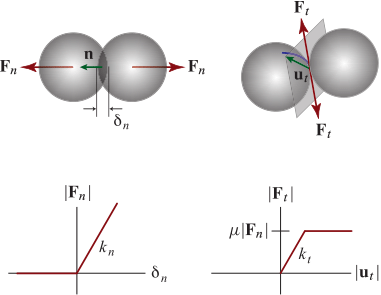
\includegraphics[width=0.8\columnwidth]{Figs/DEM-PM_Contact_Model.png}
	\caption{\small Reproduced from \protect\cite{Chrono2016}. DEM-P contact model with normal overlap distance $\delta_n$, contact-normal unit vector $\boldsymbol{n}$, and tangential displacement vector $\boldsymbol{u}_t$ (top), and a Hookean-linear contact force-displacement model with constant Coulomb sliding friction (bottom) }  
	\label{fig:Penalty}
\end{figure}

An example of a DEM-P contact constitutive law similar to one implemented in {\CHRONO} is a viscoelastic model based on either Hookean or Hertzian contact theory outlined in Equations \eqref{e:normalContact}-\eqref{e:tangentContact}. Here $\boldsymbol{u} = \boldsymbol{u}_n + \boldsymbol{u}_t$ is the overlap or local contact displacement of two interacting bodies. The quantities $\bar{m} = m_i m_j/\left(m_i + m_j\right)$ and $\bar{R} = R_i R_j/\left(R_i + R_j\right)$ are the effective mass and effective radius of curvature respectively for bodies $i$ and $j$ in contact. The vectors $\boldsymbol{v}_n$ and $\boldsymbol{v}_t$ are the normal and tangential components respectively of the relative velocity at the contact point. For a Hookean contact model, $f\left(\bar{R},\delta_n\right) = 1$ while for a Hertzian contact model, $f\left(\bar{R},\delta_n\right) = \sqrt{\bar{R}\delta_n}$ \cite{silbert2001granular,zhang2005jamming,MachadoMoreiraFloresLankarani2012}. The normal and tangential stiffnesses and damping coefficients $k_n$, $k_t$, $\gamma_n$, and $\gamma_t$ are obtained through various constitutive laws derived from contact mechanics and physically measurable properties of materials of the contacting bodies such as Young's Modulus, Poisson's ratio, coefficient of restitution, etc. 
%
\begin{equation}\label{e:normalContact}
\boldsymbol{F}_n = f\left(\bar{R},\delta_n\right)\left(k_n \boldsymbol{u}_n - \gamma_n \bar{m}\boldsymbol{v}_n\right)
\end{equation}
%
\begin{equation}\label{e:tangentContact}
\boldsymbol{F}_t = f\left(\bar{R},\delta_n\right)\left(-k_t \boldsymbol{u}_t - \gamma_t \bar{m}\boldsymbol{v}_t\right)
\end{equation}

The component of the contact displacement vector $\boldsymbol{u}$ in the contact normal direction $\boldsymbol{u}_n = \delta_n \boldsymbol{n}$ is obtained directly from the contact detection algorithm which identifies and quantifies the magnitude of body overlap between interacting bodies. The tangential contact displacement vector $\boldsymbol{u}_t$ is a bit more complicated and formulated in Equation \eqref{e:TangentialContactHistory}. In Equation \eqref{e:TangentialContactHistory}, $t$ is the current time and $t_0$ is the time when the contact was initiated. Then for a true tangential contact displacement history model,the vector $\boldsymbol{u}_t$ must be stored and updated at each time for each contact point from the time when contact is initiated up until the contact is terminated. A visualization of the Penalty method is presented in Figure \ref{fig:Penalty}. 
%
\begin{equation}\label{e:TangentialContactHistory}
\boldsymbol{u}_t = \int_{t_0}^{t}\boldsymbol{v}_t dt - \left( \boldsymbol{n}\cdot  \int_{t_0}^{t}\boldsymbol{v}_t dt \right)  \boldsymbol{n}
\end{equation}

To enforce the Coulomb friction law, if $\lvert \boldsymbol{F}_t \rvert > \mu\lvert \boldsymbol{F}_n \rvert$ at any given time step, before the contact forces are added to the resultant force and torque on each body, the stored value of $\lvert\boldsymbol{u}_t\rvert$ is scaled such that $\lvert \boldsymbol{F}_t \rvert = \mu\lvert \boldsymbol{F}_t \rvert$, where $\mu$ is the Coulomb friction coefficient. An example of this is presented in Equation \eqref{e:tanLimit} if a Hookean contact model is used and $ f\left(\bar{R},\delta_n\right) = 1$ in Equations \eqref{e:normalContact} and \eqref{e:tangentContact}.
%
\begin{equation}\label{e:tanLimit}
k_t\lvert \boldsymbol{u}_t \rvert > \mu\lvert \boldsymbol{F}_n \rvert  \Rightarrow \boldsymbol{u}_t \leftarrow \boldsymbol{u}_t \frac{\mu\lvert \boldsymbol{F}_n \rvert}{k_t\lvert \boldsymbol{u}_t \rvert}
\end{equation}

Through the processes described above, once the contact forces $\boldsymbol{F}_n$ and $\boldsymbol{F}_t$ are computed for each contact and their contributions are summed to obtain resultant forces and torques for each interacting body, the Newton-Euler equations of motion are integrated subject to the Courant-Friedrichs-Lewy (CFL) stability condition. The CFL stability condition limits the integration time step-size to $h<h_{crit} \sim \sqrt{m_{min} / k_{max}}$  \cite{OSullivan&Bray2004}. For multibody dynamics simulations with frictional contact modeled using the penalty approach as with this research, {\CHRONO} implements index 3 DAE solutions \cite{Chrono2016}.

%%-------------------------------------------------------------

\section{{\CHRONO} Multibody Physics Package}\label{s:Chrono}

The physics modeling and simulation capabilities are provided by the multiphysics open-source package {\CHRONO}~\cite{Chrono2016}. The core functionality of {\CHRONO} provides support for the modeling, simulation, and visualization of rigid multibody systems, with additional capabilities offered through optional modules. These modules provide support for additional classes of problems (e.g., finite element analysis and fluid-solid interaction), for modeling and simulation of specialized systems (such as ground vehicles and granular dynamics problems), or provide specialized parallel computing algorithms (multi-core, GPU, and distributed) for large-scale simulations.

%% ------------------------------------------------------------

\subsection{Vehicle Modeling}\label{ss:Chrono_Vehicle}
	
Built as a {\CHRONO} extension module, {\ChronoVehicle}~\cite{ChronoVehicle_TR} is a C++ middleware library focused on the modeling, simulation, and visualization of ground vehicles.
%
{\ChronoVehicle} provides a collection of templates for various topologies of both wheeled and tracked vehicle subsystems, as well as support for modeling of rigid, flexible, and granular terrain, support for closed-loop and interactive driver models, and run-time and off-line visualization of simulation results.

Modeling of vehicle systems is done in a modular fashion, with a vehicle defined as an assembly of instances of various subsystems (suspension, steering, driveline, etc.).  Flexibility in modeling is provided by adopting a template-based design. In {\ChronoVehicle}, templates are parameterized models that define a particular implementation of a vehicle subsystem. As such, a template defines the basic modeling elements (bodies, joints, force elements), imposes the subsystem topology, prescribes the design parameters, and implements the common functionality for a given type of subsystem (e.g., suspension) particularized to a specific template (e.g., double wishbone). Finally, an instantiation of such a template is obtained by specifying the template parameters (hardpoints, joint directions, inertial properties, contact material properties, etc.) for a concrete vehicle (e.g., the HMMWV front suspension).

For wheeled vehicle systems, templates are provided for the following subsystems:
{\em suspension} (double wishbone, reduced double wishbone using distance constraints, multi-link, solid-axle, McPhearson strut, semi-trailing arm);
{\em steering} (Pitman arm, rack-and-pinion);
{\em driveline} (2WD and 4WD shaft-based using specialized {\CHRONO} modeling elements, simplified kinematic driveline);
{\em wheel} (simply a carrier for additional mass and inertia appended to the suspension's spindle body);
{\em brake} (simple model using a constant torque modulated by the driver braking input).

In addition, {\ChronoVehicle} offers a variety of tire models and associated templates, ranging from rigid tires, to empirical and semi-empirical models (such as Pacejka and Fiala), to fully deformable tires modeled with finite elements (using either an Absolute Nodal Coordinate Formulation or a co-rotational formulation).  Driver inputs (steering, throttle, and braking) are provided from a {\em driver} subsystem with available options in {ChronoVehicle} including both open-loop (interactive or data-driven) and closed-loop (e.g., path-following based on PID controllers).

%% ------------------------------------------------------------

\section{MPC LIDAR-Based Local Obstacle Avoidance: History and Current Algorithm}\label{s:MPC}

The concept of MPC is to use an internal model of the system one desires to control to predict and optimize future system behavior from the current system state and inputs ~\cite{Allgower&Findeisen2002}. The system behavior is predicted over some defined finite time horizon and the optimal control sequence over the prediction horizon is output. The control sequence is executed for an execution time smaller than the prediction horizon, and the whole process is repeated. The repetition of this process over time creates a feedback loop which continually controls the system, pushing it towards an optimal path.

\begin{figure}
	\centering
	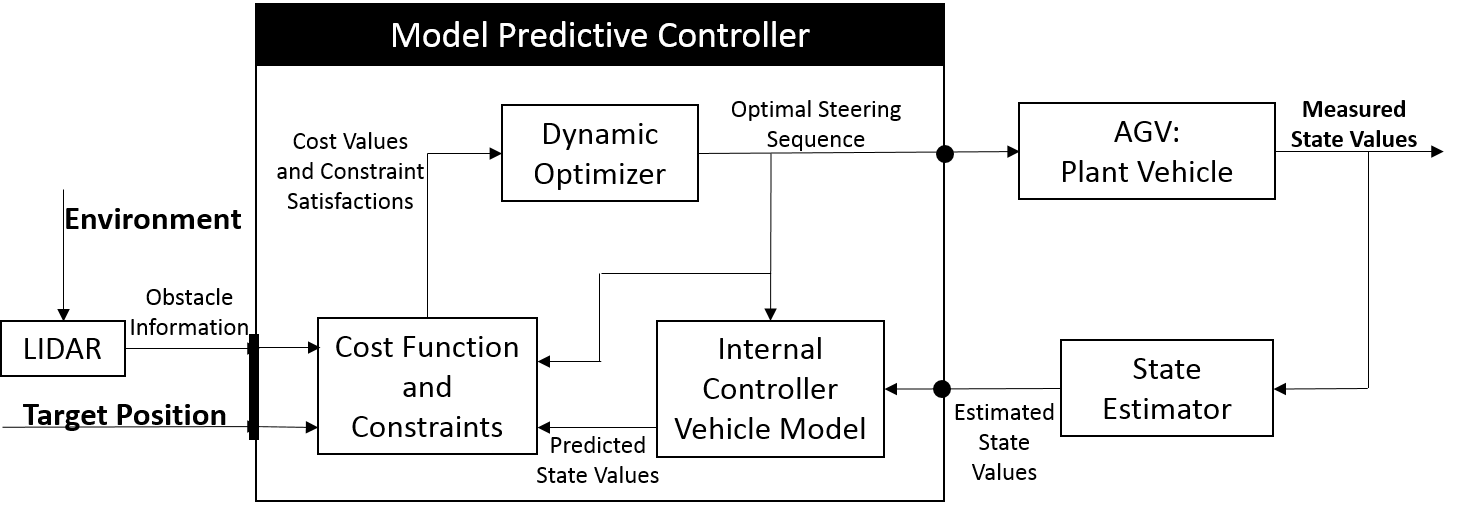
\includegraphics[width=0.9\textwidth]{Figs/MPCBlockDiagram.png}
	\caption{{\small Schematic of MPC LIDAR-Based Constant Speed Local Obstacle Avoidance Controller}}    
	\label{fig:MPC_schematic}
\end{figure}

For this study, the system to be controlled is an AGV. Consider an AGV located in a level environment without roads or any other structures to guide its motion and assume the AGV has a known global target position. Between the target position and the current vehicle position there may or may not be obstacles of unknown size. Using the MPC formulation outlined in~\cite{ModelFidelity2016}, the vehicle can navigate from the current position to the provided target position while avoiding obstacles as they are encountered. Obstacle information is assumed to be unknown a priori and only obtained through a planar LIDAR sensor. The MPC schematic is presented in Figure~\ref{fig:MPC_schematic}.
%

The planar LIDAR sensor, mounted at the front center location of the vehicle, returns the closest obstacle boundary in all radial directions of the sensor at an angular resolution $\epsilon$. The sensor has a maximum range past which it cannot sense any obstacles. Therefore, if the closest obstacle boundary is greater than the LIDAR radius $R_{LIDAR}$, then the sensor returns $R_{LIDAR}$. The LIDAR sensor range is [$0^\circ$, $180^\circ$], with $90^\circ$ being the vehicle heading direction. Since the AGV considered here is driving along level ground, whether granular or rigid, a planar LIDAR sensor is sufficient. The sensor is assumed to have no delay and zero noise and can therefore instantaneously generate a safe area polygon assembled from the returned points from the LIDAR. An overhead view of the AGV encountering an obstacle and the generated LIDAR safe area polygon are presented in Figure~\ref{fig:LIDARExample}. 
%

\begin{figure}[t]
	\centering
	\begin{subfigure}[t]{0.45\textwidth}
		\centering
		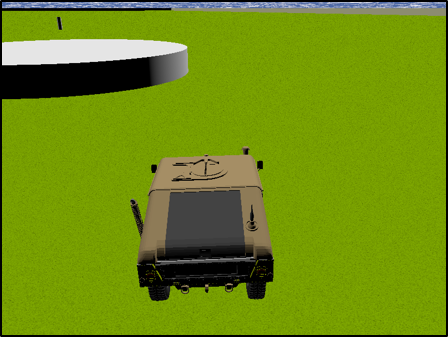
\includegraphics[width=\columnwidth]{Figs/incomingObst.png}
		\caption{{\small 3D Visualization of LIDAR Encountering Obstacle}}   
		\label{fig:obstacle_field_3D}
	\end{subfigure}
	\hfill
	\begin{subfigure}[t]{0.45\textwidth}
		\centering
		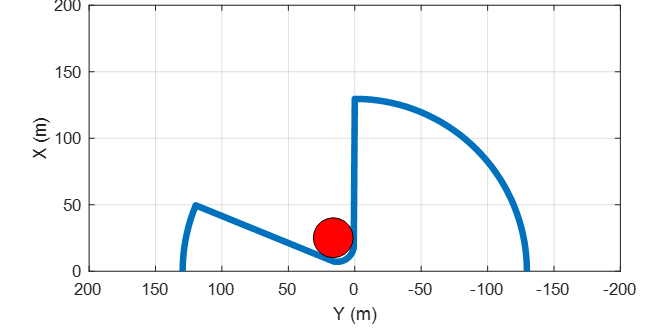
\includegraphics[width=\columnwidth]{Figs/obstLIDAR.png}
		\caption{\small LIDAR Sensed Safe Area}   
		\label{fig:obstacle_field_LIDAR}
	\end{subfigure}
	\caption{\small Sample obstacle field and LIDAR output}
	\label{fig:LIDARExample}
\end{figure}

In this research, all of the obstacles are upright cylinders so a ray-circle intersection algorithm is used to determine when each LIDAR ray intersects with a nearby obstacle. The ray-circle intersection algorithm is developed as follows. Consider a two dimensional ray in the x-y plane with the start point $\boldsymbol{E}$ and $\boldsymbol{L}$ some point along the length of the ray we are interested in. In our case, this point is the LIDAR radius. Also consider a circle with a center point defined as $\boldsymbol{C}$ and radius $r$. This is visualized in Figure \ref{fig:RayCircleIntersection}. We then form the following vectors:

\begin{figure}
	\centering
	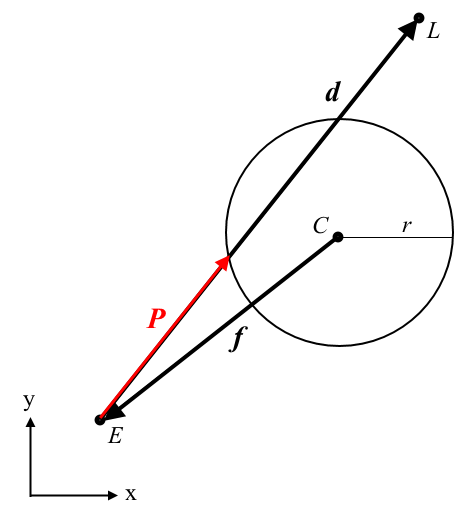
\includegraphics[width=0.5\textwidth]{Figs/rayCircle.png}
	\caption{{\small Ray-Circle Intersection Visualization}}    
	\label{fig:RayCircleIntersection}
\end{figure}
%
\begin{equation}\label{e:RayVector}
\boldsymbol{d} = \boldsymbol{L} - \boldsymbol{E}
\end{equation}
\begin{equation}\label{e:CircleCenterVector}
\boldsymbol{f} = \boldsymbol{E} - \boldsymbol{C} 
\end{equation}
\begin{equation}\label{e:Intersection}
\boldsymbol{P} = \boldsymbol{E} + t\boldsymbol{d}
\end{equation}

Here, $\boldsymbol{d}$ is a vector describing the ray from its start point to end point. $\boldsymbol{f}$ is a vector from the circle center to the start of the vector $\boldsymbol{d}$. $\boldsymbol{P}$ is the location of the point where the ray intersects with the circle. $t$ is a scalar which defines how far along the length of $\boldsymbol{d}$ the intersection between the ray and the circle actually occurs. The circle is then defined by:
%
\begin{equation}\label{e:Circle}
\left(x - C_{x}\right)^{2} +   \left(y - C_{y}\right)^{2} = r^2
\end{equation}
\begin{equation}\label{e:CircleExpanded}
x^2 - 2C_{x}x + C_{x}^{2} + y^2 - 2C_{y}y+ C_{y}^{2} - r^2 = 0
\end{equation}

We seek the point or points where the ray intersects with this circle which also happens to be described by Equation \eqref{e:Intersection} as well. Noting this yields:
%
\begin{equation}\label{e:XIntersection}
x = E_{x} + td_{x} 
\end{equation}
\begin{equation}\label{e:YIntersection}
y = E_{y} + td_{y} 
\end{equation}

Substituting Equations \eqref{e:XIntersection} and \eqref{e:YIntersection} into \eqref{e:CircleExpanded} results in the following.
%
\begin{equation}\label{e:CircleSubst}
\left(E_{x} + td_{x}\right)^2 - 2C_{x}\left(E_{x} + td_{x}\right) + C_{x}^{2} + \left(E_{y} + td_{y}\right)^2 - 2C_{y}\left(E_{y} + td_{y}\right)+ C_{y}^{2} - r^2 = 0
\end{equation}

Expanding and grouping like terms yields the following.
%
\begin{equation}\label{e:CircleGrouped}
t^{2}\left(d_{x}^{2} + d_{y}^{2}\right) + 2t\left(E_{x}d_{x} + E_{y}d_{y} - C_{x}d_{x} - C_{y}d_{y}\right) + E_{x}^{2} + E_{y}^{2} - 2 E_{x}C_{x} - 2 E_{y}C_{y} + C_{x}^{2} + C_{y}^{2} - r^{2} = 0
\end{equation}

Equation \eqref{e:CircleGrouped} can be simplified further by identifying previously defined vectors and dot products can be substituted in.
%
\begin{equation}\label{e:RayCircleIntersection}
t^{2}\left(\boldsymbol{d}\cdot\boldsymbol{d}\right) + 2t\left(\boldsymbol{f}\cdot\boldsymbol{d}\right) +\boldsymbol{f}\cdot\boldsymbol{f} - r^{2} = 0
\end{equation}

Equation \eqref{e:RayCircleIntersection} is a quadratic equation that can be solved for two values of $t$. The ray-circle intersection algorithm then implemented for this research checks the discriminant of Equation \eqref{e:RayCircleIntersection}. If the discriminant is less than zero, then the roots of this quadratic are imaginary and there is no intersection with the circle. If the discriminant is greater than zero, then there is an intersection and the quadratic formula is used to solve for the two values of $t$ that satisfy Equation \eqref{e:RayCircleIntersection}. Of the two solved $t$ values, the lower value is checked to see if it is less than one but greater than zero. If so, this $t$ value is the ray-circle intersection point used as the LIDAR detected point for the algorithm for this specific ray. Otherwise, the algorithm returns the maximum LIDAR radius. This algorithm does a quick and efficient job of simulating a perfect LIDAR sensor when the algorithm is performed on a set of rays all sweeping iteratively from the vehicle's location.

For the purpose of these simulations, the only outputs of the MPC algorithm are the steering signals. As shown in Figure~\ref{fig:MPC_schematic}, the MPC algorithm is made up of the internal controller vehicle model, the cost function and constraints, and the dynamic optimizer. The internal controller vehicle model predicts the future states of the AGV for a given steering sequence. Herein, the internal controller vehicle model is varied from test to test between a 2-DOF vehicle model and a 14-DOF vehicle model, as detailed in further sections. Cost functions and constraints are used to formulate the optimal control problem using the equations from the vehicle model, and the resulting optimal control problem is solved using dynamic optimization.

Since the ability of finding and executing an optimal solution, rather than solution speed, is the primary focus here, an exhaustive search is used to find the optimal solution to the problem at hand. With this method, the steering sequence is discretized and a finite set of path possibilities are tested and weighed by a cost function. 

The MPC controller as formulated in~\cite{ModelFidelity2016} is used for this study. The cost function and constraints need to be specified to avoid collisions with obstacles and guarantee vehicle dynamical safety. The optimal control problem solved at each MPC time step consists of the following set of equations:
%
\begin{equation}\label{e:MPCCost}
J = s_T + wd 
\end{equation}
\begin{equation}\label{e:State_ODE}
\dot{\xi} = v\left[\xi\left(t\right),\zeta\left(t\right)\right] 
\end{equation}
\begin{equation}\label{e:InitialStates}
\xi\left(0\right) = \xi_0 
\end{equation}
\begin{equation}\label{e:SafeArea}
\tilde{S}\left[x\left(t\right),y\left(t\right)\right] \leq0  
\end{equation}
\begin{equation}\label{e:SteerLimit}
\left|\delta_f\left(t\right)\right| \leq\tilde{\delta}_{f,max}\left(U_0\right) 
\end{equation}
\begin{equation}\label{e:SteerRateLimit}
\left|\varsigma_f\left(t\right)\right| \leq\varsigma_{f,max} 
\end{equation}
\begin{equation}\label{e:TimeDomain}
t \in \left[0,T_P\right] \,.
\end{equation}

Equation~\eqref{e:MPCCost} defines the cost function for this optimal control problem. This equation is a soft requirement which defines how the separate path possibilities are weighed against each other and how to determine which path is actually optimal. The cost function is comprised of two terms defined as:
%
\begin{equation}\label{e:DistanceCost}
s_T = \sqrt{\left[ x_G - x\left(T_P\right)\right]^2 + \left[y_G - y\left(T_P\right)\right]^2 }
\end{equation}
\begin{equation}\label{e:TurningCost}
d = \int \limits_0^{T_G} \left|\varsigma\left(t\right)\right| dt \,.
\end{equation}
%
Here, $s_{T}$ seeks to minimize the distance between the prediction end-location and the target position. A prediction path that guides the vehicle towards the closest location to the target will have the smaller $s_{T}$ term. The second term, $d$, aims to minimize the change in steering angle so that smoother, straighter paths are preferred over windy paths. A weighting factor $w$ is used to scale the influence of $d$ in the total cost.

Equations~\eqref{e:State_ODE}-\eqref{e:TimeDomain} are the constraints for this optimal control problem and represent hard requirements for vehicle safety and collision avoidance. Any paths that violate these constraints are not considered safe paths and are eliminated as potential options in this prediction window. Equation~\eqref{e:State_ODE} defines a set of differential equations that describe the internal controller vehicle model, with the initial conditions of Equation~\eqref{e:InitialStates}.

Equation~\eqref{e:SafeArea} defines a safe area polygon, constructed from LIDAR data and including an additional safety buffer to account for vehicle size and to prevent collisions of the vehicle corners.  All points along paths found from Equations~\eqref{e:State_ODE})-(\eqref{e:InitialStates} must fall inside this safe area polygon.

Equation~\eqref{e:SteerLimit} imposes a maximum limit on the steering angle, based on vehicle speed. This value is obtained from a lookup table which can be generated either experimentally or from simulation. Equation~\eqref{e:SteerRateLimit} imposes a maximum limit on steering rate. Equation~\eqref{e:TimeDomain} defines the time limits over which this optimal control problem is solved.

As noted above, Equation~\eqref{e:State_ODE} refers to an analytical vehicle model expressed as a set of differential equations which allow the controller to predict vehicle performance within the prediction horizon. The accuracy of the internal vehicle controller model should directly influence the driven vehicle's controlled performance. If the internal vehicle controller model poorly predicts a vehicle's response to inputs from the driver or the environment, then these deficiencies will be witnessed when attempting to control the driven vehicle and result in incorrect trajectories that may lead to collisions. On the other hand, a highly complex internal vehicle controller model may provide accurate trajectory and vehicle response predictions, but with an unacceptable time required to solve the optimal control problem. An ideal controller should not only accurately predict vehicle responses, but also do it quickly enough to insure vehicle safety. 
%%
In this study we consider two separate internal controller vehicle models to approximate the dynamics of the driven {\CHRONO} HMMWV vehicle (described in Chapter~\ref{c:ExpSetup}).  The first controller uses a simple 2-DOF vehicle model to predict the trajectory for different series of steering sequences and is presented in detail in Section~\ref{ss:2DOFModel}. The second controller, described in Section~\ref{ss:14DOFModel}, uses a more complex 14-DOF vehicle model. These two models are compared in their ability to successfully navigate the driven HMMWV vehicle through two obstacle fields, on rigid flat terrain and then granular terrain.

As mentioned previously, exhaustive search space~\cite{ModelFidelity2016} is used to solve the optimal control problem at each time step. The steering space is discretized into five possible steering angles, while the prediction horizon is split into four intervals. This results in 625 different steering sequence possibilities and therefore 625 different path possibilities that are weighed by the controller to determine the optimal steering sequence and resulting forward path. A sample visualization of the different predicted trajectories from the 2-DOF model is presented in Figure~\ref{fig:PossiblePaths} where, for visualization purposes, only three steering angles over three intervals were considered. A point in polygon algorithm is used to determine which trajectories remain inside of the safe area polygon visualized in Figure ~\ref{fig:LIDARExample} and therefore should be compared to the other possibilities using Equation ~\eqref{e:MPCCost}.

\begin{figure}
	\centering
	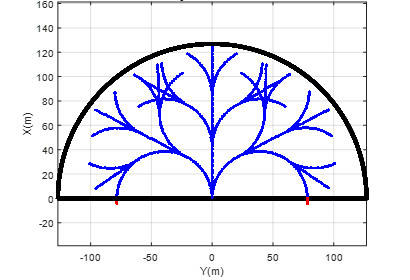
\includegraphics[width=0.8\columnwidth]{Figs/PathPossibilities.png}
	\caption{\small Potential Paths predicted by 2-DOF Internal Vehicle Controller Model}  
	\label{fig:PossiblePaths}
\end{figure}
 
To determine if any point along the path is within the LIDAR sensed safe area polygon, a point in polygon algorithm is used. The algorithm developed for this research is similar to the winding method where the winding method tracks how many times the edges of the polygon wind around the current point of interest. However, the algorithm developed and used in this research is much simpler and quicker and is very similar to that provided in \cite{pointinpolygon2014}. This algorithm checks the quadrant where each vertex of the polygon is located in a frame with origin at the current point we are testing. The algorithm then counts the number of times that quadrant changes as the algorithm cycles through all of the vertices to determine if the point of interest is inside the polygon. The motivation for this actually comes from real llife. Imagine sitting in a closed room. A way one could test if they were actually in the room would be to iteratively look at all the corners of the room in sequence. In the person's relative reference frame fixed in its orientation, cycling through the corners of the room one would note the net quadrant change is 4, regardless of how many corners there are. Now if the person were standing outside of the room and performed this same test, they would not that the net quadrant changes was a number other than 4 meaning the room did not enclose them and therefore they are outside of the room. Again the method is similar to the winding method but the algorithm performs and checks different aspects to reach the same conclusion quicker. A note is since for this research a planar LIDAR sensor is used, this algorithm is only developed in two dimensions in the x-y plane. 

To start, the polygon is simply an ordered list of its vertices. Edges are line segments connecting one vertex to the next. The first vertex of the list and the last vertex of the list are also connected to close the polygon.   Next, we consider a reference frame at the point we are testing and express all of the vertices in this relative reference frame. The first vertex is chosen and the quadrant that it resides in is identified. Then the next vertex is chosen and its quadrant is identified as well. If the two points fall in the same quadrant, then nothing happens and the next vertex in the list is checked. However, if the quadrant is different from the previous vertex quadrant, this change is noted and a net quadrant change counter records this change. Clockwise is positive so changes in this direction result in +1 being added to the net quadrant change counter while counterclockwise changes result in -1 being added to the counter. In the case where the quadrant changes by two such as quadrant 1 changes to 3 or 2 to 4 or vice versa, a vector is expressed connecting the old vertex and new vertex. Depending on the direction of the vector and if the y-intercept is above or below zero determines if +2 or -2 is added to the net quadrant change counter. Once the algorithm cycles through all of the vertices, it checks the original vertex in order to close the polygon. If the net quadrant change is 4 or -4, then the point is in the polygon. Any other situation means the point is outside of the polygon. This algorithm is efficient, simple, and has been implemented successfully for use in this research. However, this algorithm would need to be rethought for application in 3D space. Figure \ref{fig:PointInPolygon} presents a set of sample points used to show the algorithm effectively checks to see if the points fall within a sample LIDAR safe area polygon.

\begin{figure}
	\centering
	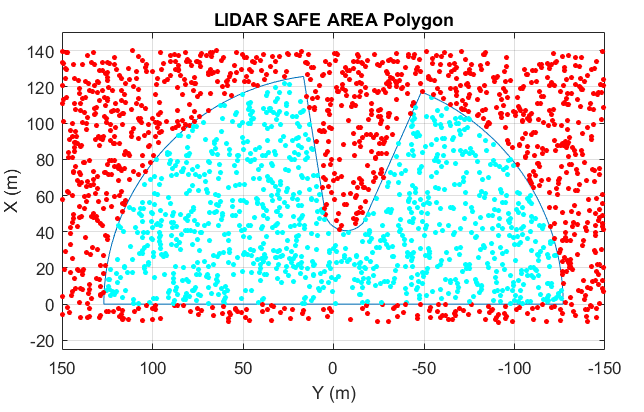
\includegraphics[width=0.7\columnwidth]{Figs/PointInPolygon.png}
	\caption{\small Visualization of Point in Polygon Algorithm Working Successfully}  
	\label{fig:PointInPolygon}
\end{figure}

%% ------------------------------------------------------------

\section{Multi-DOF Vehicle Dynamics Models}\label{s:IntModel}

The vehicle models embedded in the MPC are simplifications of the full, multi-body based, {\CHRONO} wheeled vehicle model which is being controlled.  Two models were considered initially, providing different levels of fidelity, as described below.

%% ------------------------------------------------------------

\subsection{2-DOF Vehicle Model}\label{ss:2DOFModel}
The standard vehicle model used in recently developed MPC obstacle avoidance algorithms such as~\cite{ModelFidelity2016} is the 2-DOF yaw plane vehicle model. These models normally either assume constant cornering stiffness or the nonlinear Pacejka Magic Formula Tire Model~\cite{Pacejka2012} to predict the ground tire interaction forces. For this study, the Pacejka Magic Formula is used to predict tire forces in the vehicle models. This force model is presented in the future Section \ref{s:Pacejka}.   

A visual representation of the 2-DOF yaw plane vehicle model can be found in Figure~\ref{fig:2DOF}. The 2-DOF model is described by the following first-order ordinary differential equations:
%
\begin{equation}\label{e:2DOF_Vdot}
\dot{V} = \left(F_{y,f} + F_{y,r}\right)/{M - U_0r} 
\end{equation}
\begin{equation}\label{e:2DOF_rdot}
\dot{r} = \left(F_{y,f}L_f - F_{y,r}L_r\right)/I_{zz}
\end{equation}
\begin{equation}\label{e:2DOF_psidot}
\dot{\psi} = r 
\end{equation}
\begin{equation}\label{e:2DOF_xdot}
\dot{x} = U_0\cos{\psi}-\left(V+L_fr\right)\sin{\psi}
\end{equation}
\begin{equation}\label{e:2DOF_ydot}
\dot{y} = U_0\sin{\psi}+\left(V+L_fr\right)\cos{\psi} \,,
\end{equation}
%
where $F_{y,f}$ and $F_{y,r}$ are the lateral tire forces at the front and rear axles, respectively. $U_0$ and $V$ are the longitudinal speed and lateral speed of the vehicle in the vehicle's coordinate frame. $\psi$ is the yaw angle and $r$ is the yaw rate. $\left(x,y\right)$ represent the front center location of the vehicle expressed in global coordinates. $M$ is vehicle mass, $I_{zz}$ is the moment of inertia of the vehicle, $L_f$ is the distance from the front axle to the vehicle CoG, and $L_r$ is the distance from the rear axle to the vehicle CoG. For this research, the model is constrained to a constant longitudinal speed. Then the planar 3-DOF body with one constraint results in the 2-DOF model used for this study.

\begin{figure}
	\centering
	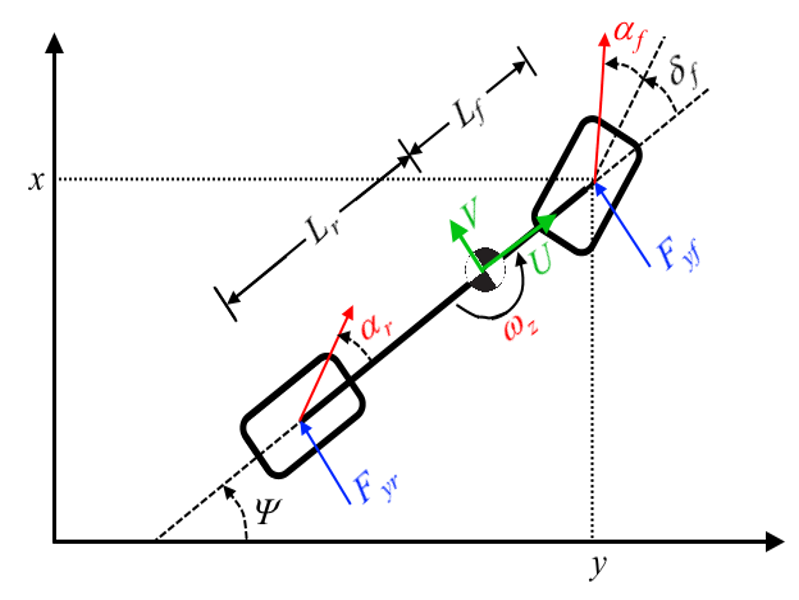
\includegraphics[width=0.8\columnwidth]{Figs/2DOF_haraus.png}
	\caption{\small 2-DOF Vehicle Model}  
	\label{fig:2DOF}
\end{figure}

%% ------------------------------------------------------------

\subsection{14-DOF Vehicle Model}\label{ss:14DOFModel}
A 14-DOF model is often used in studies such as these to test the obstacle avoidance controller with a higher fidelity vehicle model~\cite{ModelFidelity2013, ModelFidelity2016}. A benefit of using the 14-DOF in the controller is the model's ability to predict tire liftoff and account for dynamic effects from suspension systems. For this research, it is appropriate to also compare performance of the local obstacle avoidance controller running an internal 14-DOF on rigid terrain versus granular terrain.  

The 14-DOF vehicle model consists of one sprung mass connected above four unsprung masses~\cite{RollStudies2007}. The sprung mass is allowed to roll, pitch, and yaw while also displacing laterally, vertically, and longitudinally. This sprung mass contributes six DOF to the model. Each of the four wheels are allowed to bounce vertically and rotate about the wheel horizontal axis. The front two wheels are also free to steer. Each wheel then contributes two DOF to the 14-DOF model. The model is constrained at a constant longitudinal speed of 8.1 m/s. The equations used for this model, as well as their derivation can be found in~\cite{RollStudies2007} and visualized in Figure \ref{fig:14DOF}.

\begin{figure}
	\centering
	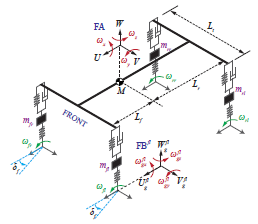
\includegraphics[width=0.8\columnwidth]{Figs/14DOF_Stein.png}
	\caption{\small Reproduced from \protect\cite{RollStudies2007}. 14-DOF Vehicle Model}  
	\label{fig:14DOF}
\end{figure}

%%-------------------------------------------------------------
\section{Tire Ground Force Model: Pacejka Magic Formula}\label{s:Pacejka}

The Pacejka Magic Formula is a semi-empirical tire model developed in 1987 by Hans B. Pacejka from Delft University of Technology, Egbert Bakker from Volvo Cars, and Lars Nyborg from Volvo Cars \cite{TireSensitivityStudy}. This model was developed further by Pacejka and commercially known as the "MF-Tire." The Magic Formula is capable of characterizing a tire with a large set of coefficients obtained from experiments. These coefficients are then used to calculate lateral, longitudinal forces as well as the self aligning torque experienced by a tire interacting with the ground. 
%
\begin{equation}\label{e:MagicA}
A = B\left(F_z\right)\cdot\alpha 
\end{equation}
\begin{equation}\label{e:MagicLateral}
F_y = D\left(F_z\right)\cdot sin\left\{C\left(F_z\right)\cdot atan\left[A-E\left(F_z\right)\cdot A+E\left(F_z\right)\cdot atan\left(A\right)\right]\right\}
\end{equation}

The lateral forces at a wheel used in the previously described 2-DOF vehicle model are calculated using Equations \eqref{e:MagicA} and \eqref{e:MagicLateral} for the case of pure lateral slip.  $F_{z}$ is the vertical load at the axle. $\alpha$ is the lateral tire slip angle. $B\left(\cdot\right)$, $C\left(\cdot\right)$, $D\left(\cdot\right)$, and $E\left(\cdot\right)$ are functions of the tire vertical load $F_{z}$ and these relationships are described in \cite{Pacejka2012}. The slips at a front and rear tire are calculated using Equations \eqref{e:SlipFront} and \eqref{e:SlipRear} respectively where $\delta_f$ is the steering angle of the front wheel.
%
\begin{equation}\label{e:SlipFront}
\alpha_f = tan^{-1}\left( \frac{V+L_{f}r}{U_0} - \delta_f\right) 
\end{equation}
\begin{equation}\label{e:SlipRear}
\alpha_r = tan^{-1}\left( \frac{V-L_{r}r}{U_0}\right)
\end{equation}

The tire vertical load is then required as an input to Equations \eqref{e:MagicA} and \eqref{e:MagicLateral}. Longitudinal load transfer is accounted for when calculating front and rear tire vertical loads. Justification for this inclusion can be found in \cite{ModelFidelity2016}. Equations \eqref{e:FrontLoad} and \eqref{e:RearLoad} are then used to calculate the front and rear tire loads $F_{z,f}$ and $F_{z,r}$ and input into Equations \eqref{e:MagicA} and \eqref{e:MagicLateral}.
%
\begin{equation}\label{e:FrontLoad}
F_{z,f}= \frac{MgL_r + MVrh_CG}{L_f+L_r} 
\end{equation}
\begin{equation}\label{e:RearLoad}
F_{z,r}= \frac{MgL_f - MVrh_CG}{L_f+L_r} 
\end{equation}

The Magic Formula characterizes the tire's interaction with rigid ground with a set of coefficients and uses those coefficients to match the Magic Formula with experimental data. Then a tire interacting with one type of pavement will have different Magic Formula parameters than the same tire interacting with a different type of pavement. However, the Magic Formula models tire ground interactions on rigid ground, not granular terrain i.e. there is not a granular terrain Magic Formula. There is then a mismatch between the internal controller models and the plant vehicle when controlling the vehicle on granular terrain, but this research first seeks to identify what role that mismatch plays in controller performance. Improvements presented in Chapter \ref{c:improvedModel} address this model mismatch in order to better account for the granular terrain interaction.

%%-------------------------------------------------------------
\section{Optimization Problem: Exhaustive Search Space}\label{s:Optimization}

When this controller is implemented in real-time on a physical vehicle, it will use some high efficiency optimization algorithm to compute which steering sequence is best for the HMMWV to follow. For this research, that is not the case because the interest lies in analyzing the role and effect of model fidelity on the controller performance. When the system dynamics are represented using the 14-DOF analytical vehicle model, the optimization problem becomes very difficult to solve and the techniques to perform this are still the subject of ongoing research. Considering this observation, an exhaustive search space approach is used for this research to solve the optimal control. This is the same technique used in \cite{ModelFidelity2016}. 

\begin{figure}
	\centering
	\begin{subfigure}[t]{0.49\columnwidth}
		\centering
		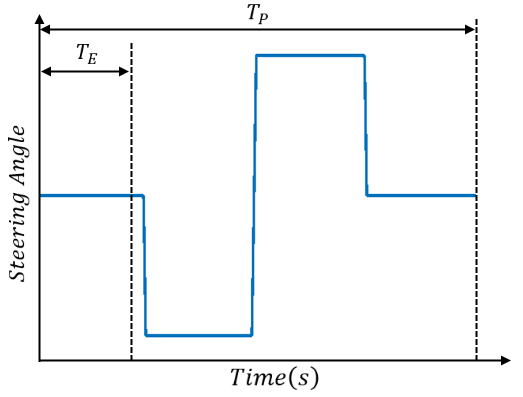
\includegraphics[width=\columnwidth]{Figs/steeringSequence.png}
		\caption{{\small Sample Steering Sequence}}   
		\label{fig:Paths}
	\end{subfigure}
	\hfill
	\begin{subfigure}[t]{0.49\columnwidth}
		\centering
		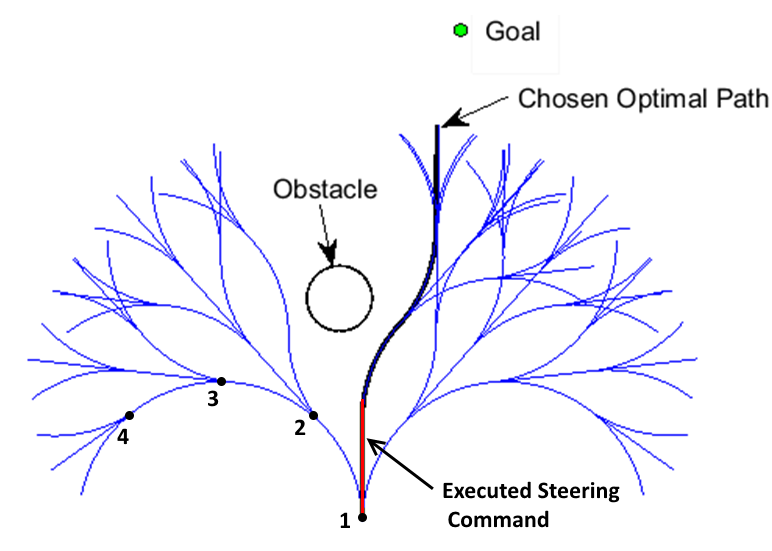
\includegraphics[width=\columnwidth]{Figs/exhaustObst.png}
		\caption{\small Visualization of Exhaustive Search Method using $n_s=3$ and $n_p=4$}   
		\label{fig:PathsSafe}
	\end{subfigure}
	\caption{\small Exhaustive Search Space Simplified Visualization}
	\label{fig:SimplePaths}
\end{figure}

Using this exhaustive search space method, the steering search space is discretized instead of considering the entire continuous steering search space. Some discrete steering angles are considered which include the maximum safe steering angle, negative maximum steering angle, and zero steering. The set of discrete steering angles is then denoted as the steering angle pool, represented by Equation \eqref{e:steerPool}. The prediction horizon is divided into intervals of equal length. Then at each interval, a steering angle from the steering pool is selected and held constant for that interval. A zero-order hold approach is used to develop a steering angle sequence from the steering angle of each interval. Ramp transitions join two different steering angles so that the slope is the maximum steering rate. The prediction horizon is divided into $n_p$ intervals and the number of steering angles considered in the steering pool is $n_s$. Therefore the total size of the search space or number of different possible steering sequences considered is $n_s^{n_p}$. The steering sequence is then executed over the execution horizon $T_E$ which is set equal to or less than the interval length $T_P/n_p$. For this research, the parameters used are $n_p = 4$, $n_s=5$, and $T_E = 0.5s$. The discretization of the search space allows for a simplification of Equation \eqref{e:TurningCost} from the cost function which yields Equation \eqref{e:TurningCostDiscrete}.
%
\begin{equation}\label{e:steerPool}
\bigcirc_{steer}=[ -\tilde{\delta}_{f,max}\left(U_0\right)\cdot\cdot\cdot 0 \cdot\cdot\cdot \tilde{\delta}_{f,max}\left(U_0\right) ]
\end{equation}
\begin{equation}\label{e:TurningCostDiscrete}
d = \sum\limits_{i=1}^{n_p}|\delta_i -\delta_{i-1}|
\end{equation}

\begin{figure}
	\centering
	\begin{subfigure}[t]{0.49\columnwidth}
		\centering
		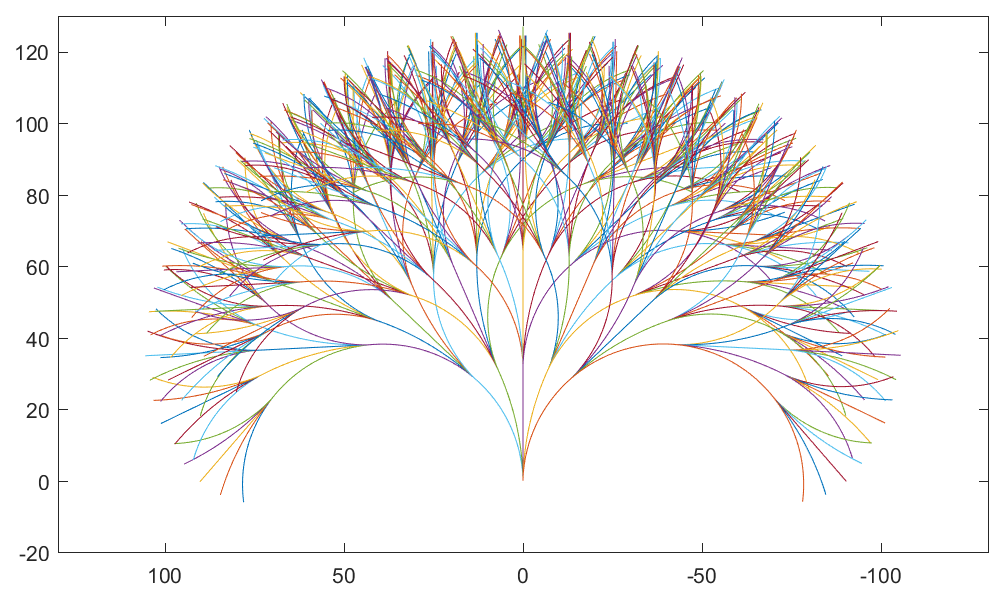
\includegraphics[width=\columnwidth]{Figs/MPCPath625.png}
		\caption{{\small All Possible Path Possibilities}}   
		\label{fig:Paths}
	\end{subfigure}
	\hfill
	\begin{subfigure}[t]{0.49\columnwidth}
		\centering
		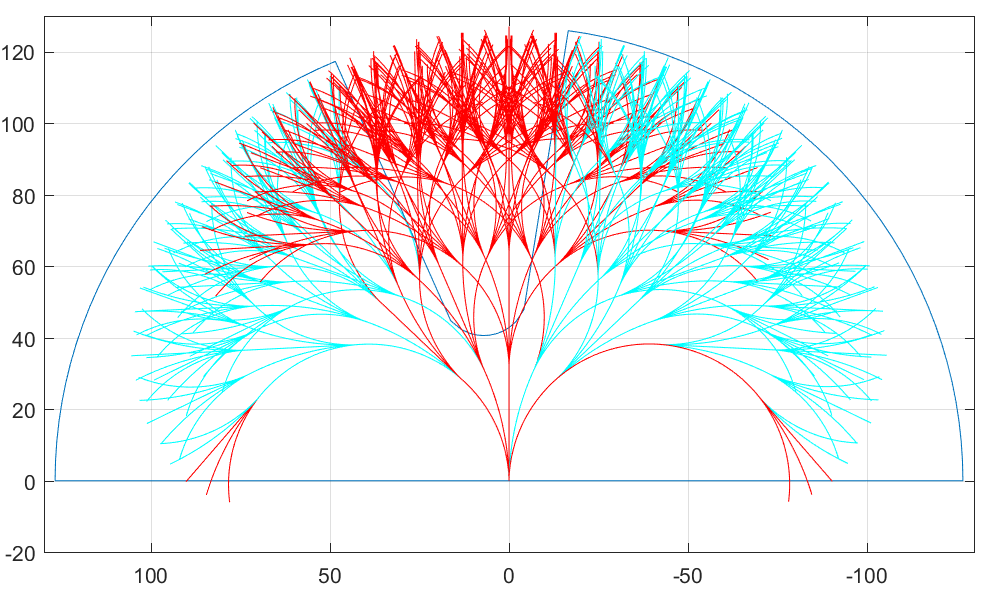
\includegraphics[width=\columnwidth]{Figs/MPCPath625_withLIDAR.png}
		\caption{\small All Path Possibilities Determined if Safe or Not}   
		\label{fig:PathsSafe}
	\end{subfigure}
	\caption{\small Exhaustive Search Space Paths Checked with Point in Polygon Algorithm}
	\label{fig:SearchPaths}
\end{figure}

The control sequences are compared against each other using the cost function. The optimal control sequence that minimizes the cost function and satisfies the constraints of the optimal control problem is selected from the steering pool and executed over the execution horizon. Starting at the initial state, control commands from the steering pool are applied to the analytical vehicle model and the resulting trajectories are checked for constraint violation. If the constraints are violated, that search branch is terminated. Else, the next step prediction is performed by using the end state of the last analytical evaluation as the new initial state and applying commands from the steering pool. This process is repeated for all intervals and until the prediction horizon window has been reached. Once all control sequences have been evaluated, they are compared using the cost function and the control sequence that minimizes the cost function is considered the optimal control sequence. The optimal control sequence is executed over the execution window and the whole process is repeated. Refer to Figure \ref{fig:SimplePaths} for an example implementation of this exhaustive search space method. Figure \ref{fig:SearchPaths} presents the full set of different path possibilities considered and how they are eliminated based on the LIDAR safe area polygon.

%%============================================================

\chapter{EXPERIMENTAL SETUP}\label{c:ExpSetup}

The model to be controlled (the {\em plant}) is a full-vehicle {\ChronoVehicle} model of a HMMWV, which includes multi-body subsystems for the suspensions, steering, driveline, and powertrain, and is available in the {\CHRONO} package.

This vehicle model (see Figure~\ref{fig:hmmwv}) has a curb weight of $2,550$~kg.
%
It includes independent front and rear double wishbone suspensions and a Pitman arm steering mechanism. The shock absorber and coil spring, mounted between the lower control arm and the chassis, are modeled with {\CHRONO} nonlinear force elements and include the effects of bump stops.
%
\begin{figure}
	\centering
	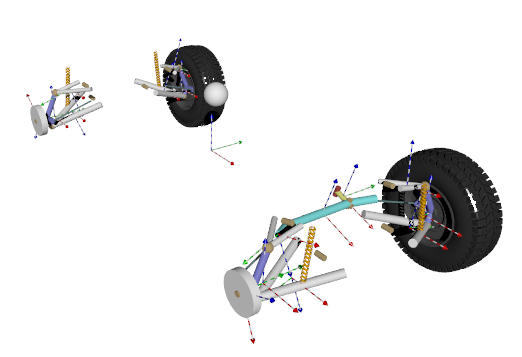
\includegraphics[width=\columnwidth]{Figs/hmmwv_bodies.png}
	\caption{\small Full-vehicle HMMWV multibody model.}  
	\label{fig:hmmwv}
\end{figure}

The AWD driveline is modeled using {\CHRONO} shaft elements and includes three power splitting elements (a central differential and front/rear differentials), as well as conical gears connected through 1-dimensional shaft elements which carry rotational inertia. 
%
The powertrain is also modeled using 1-dimensional shaft elements and includes models for a thermal engine specified through speed-torque maps for power and engine losses, a torque converter specified via maps for the capacity factor and the torque ratio, and an automatic transmission gearbox with three forward gears and a single reverse gear.
%
The connection between powertrain and driveline is a force-displacement interface at the driveshaft (with torque applied from the powertrain and angular velocity provided by the driveline).

For mobility studies on deformable terrain, provided that the tire inflation pressure is comparable or larger than the average ground pressure, according to the postulate by Wong~\cite{wong93} the tire can be considered in a so-called {\em rigid regime}.  As such, tire deformation can be ignored and the vehicle's tires are modeled using rigid contact shapes.  The HMMWV tire model used here is thus represented by a cylinder with a radius of $0.47$~m ($18.5$~in) and a width of $0.254$~m ($10$~in).

\section{Evaluation Metrics}\label{s:Metrics}
Five evaluation metrics will be used to compare one test performance to the other. First, all test runs will be compared based on the time to reach the target, $T_{target}$ to determine which controller leads the vehicle to the target point quickest. Second, the closest distance the vehicle reaches to any obstacle, $d_{min}$, will be measured. Third, the control effort will be calculated and compared between test cases. The better test case will have a lower controller effort value. Finally, the maximum and average lateral accelerations will be calculated and compared. The accelerations are calculated at the driver's position in the chassis. Using the DEM-P method of simulation results in noisy acceleration data. To address this, acceleration data is filtered to remove noise. These five evaluation metrics provide a consistent methodology for comparing one test case with another, regardless of the terrain type and underlying analytical controller model.

%%-------------------------------------------------------------

\section{Simulation Parameters}\label{s:SimParameters}

\begin{table}
\begin{center}
	\begin{tabular}{||c |c | c||} 
		\hline
		Test  & Terrain  & Controller Vehicle \\
		Number &  Type & Model\\ [0.5ex] 	
		\hline\hline
		1 & Rigid & 2-DOF \\ 
		\hline
		2 & Rigid & 14-DOF \\
		\hline
		3 & Granular & 2-DOF \\
		\hline
		4 & Granular & 14-DOF \\
		\hline
	\end{tabular}
\end{center}
\caption{Individual Simulation Test Information}
\label{t:TestMatrix}
\end{table}

Simulations on both rigid and granular terrain were compared to understand how the controller performs on non-ideal surfaces.  The two internal controller vehicle models studied in these tests were the previously described 2-DOF and 14-DOF vehicle models. All other controller parameters were kept unchanged over all tests. Referring to Table~\ref{t:TestMatrix}, the effect of model fidelity on controller performance was gauged by comparing test 1 with 2 and test 3 with 4, for rigid flat and granular terrain, respectively.
%%
Similarly, comparing test 1 with 3 and test 2 and 4 allowed evaluating the performance of each internal vehicle model on rigid and granular terrain.

\begin{figure}
	\centering
	\begin{subfigure}[b]{0.49\columnwidth}
		\centering
		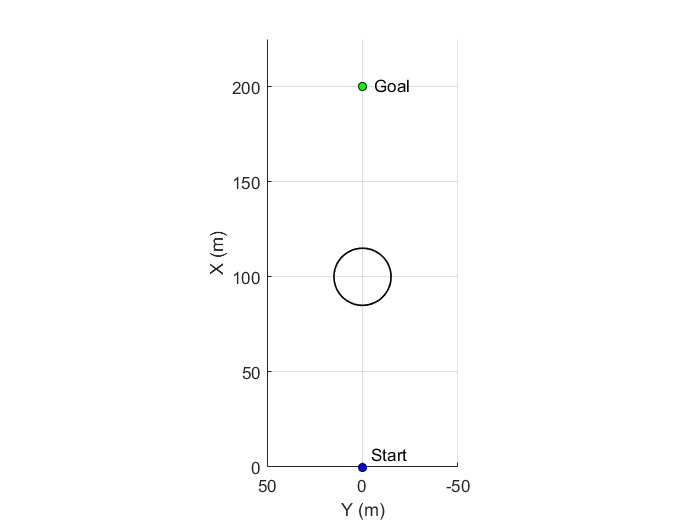
\includegraphics[width=\textwidth]{Figs/ObstacleField1.png}
		\caption{{\small Field 1}}   
		\label{fig:Obst1}
	\end{subfigure}
	\hfill
	\begin{subfigure}[b]{0.49\columnwidth}
		\centering
		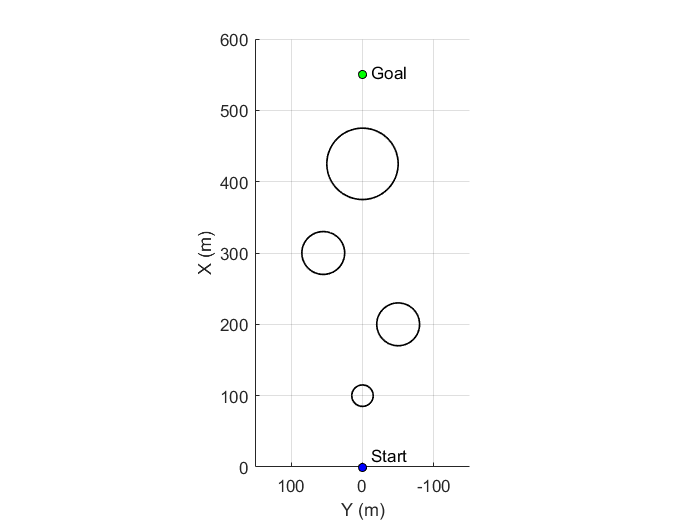
\includegraphics[width=\columnwidth]{Figs/ObstacleField2.png}
		\caption{\small Field 2}   
		\label{fig:Obst2}
	\end{subfigure}
	\caption{\small Obstacle Fields}
	\label{fig:Obst}
\end{figure}

Each of the above four tests consisted of runs on two fields with different obstacle distributions. 
%%
The first one, depicted in Figure~\ref{fig:Obst1}, contains a single large circular obstacle located along the initial heading of the vehicle, with the target location at a large distance behind the obstacle. 
%%
The second obstacle field (see Figure~\ref{fig:Obst2}) consists of four circular obstacles of varying sizes placed in the vehicle's initial heading direction, and provides a more realistic obstacle-avoidance scenario.
%%
Table~\ref{t:ObstSummary} summarizes the obstacle locations and dimensions, as well as the target location for the above two scenarios.

\begin{table}
	\begin{center}
		\begin{tabular}{||c|c|c|c||} 
			
			\hline
			& x & y & Radius\\
			& (m) & (m) & (m)\\
			\hline\hline
			\multicolumn{4}{||c||}{Field 1} \\
			\hline
			Target Location  & 200.0 & 0.0 & -\\ 
			\hline
			Obstacle 1 & 100.0 & 0.0 & 15.0\\			
			\hline\hline
			\multicolumn{4}{||c||}{Field 2} \\
			\hline
			Target Location  & 550.0 & 0.0 & -\\ 
			\hline
			Obstacle 1 & 100.0 & 0.0 & 15.0\\
			\hline
			Obstacle 2 & 200.0 & -50.0 & 30.0\\
			\hline
			Obstacle 3 & 300.0 & 55.0 & 30.0\\
			\hline
			Obstacle 4 & 425.0 & 0.0 & 50.0\\
			\hline
		\end{tabular}
	\end{center}
	\caption{Obstacle Field Parameters}
	\label{t:ObstSummary}
\end{table}

The following vehicle parameters are maintained throughout all of the executed tests. A PID speed controller is used to maintain a near constant speed of 8.1 m/s longitudinally for the simulated plant {\CHRONO} wheeled vehicle. This constant speed is also enforced in the analytical models internal to the MPC controller. The LIDAR sensor has a maximum range $R_{LIDAR} = 129.6~\text{m}$ and is sampled instantaneously at increments of $2.5^\circ$. The vehicle is limited to a maximum steering angle of $10^\circ$, with a maximum steering rate of $70^{\circ}/\text{s}$. 

%%-------------------------------------------------------------

\section{Granular Terrain Simulation}\label{s:GranSim}

Due to the large-scale nature of the simulations in this study, generating granular particles distributed across the entire obstacle field is both computationally exhausting and unreasonable. Instead, we adopt a moving-patch approach. Consider an AGV on a large terrain patch of $100$ by $100$ meters. Since we are primarily interested in the vehicle behavior and performance and not explicitly in the terrain behavior, we assume only a small patch of granular terrain underneath and around the vehicle is significant. This idea promoted the development of a relocating granular patch which enables simulations of a vehicle traversing granular terrain over a large area, without the need to generate particles everywhere throughout that area. 

\begin{figure}
	\centering
	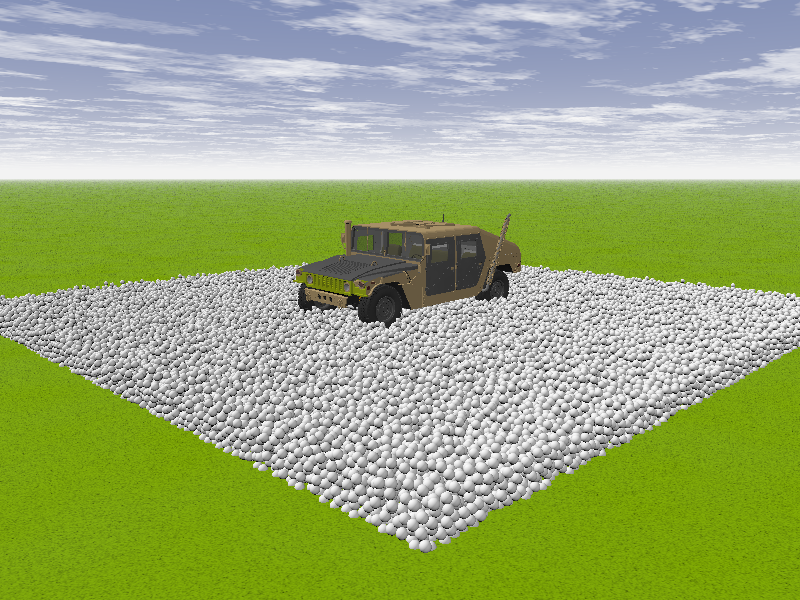
\includegraphics[width=0.8\columnwidth]{Figs/granPatch.png}
	\caption{\small Relocating Granular Patch that follows the vehicle}  
	\label{fig:granPatch}
\end{figure}

This mechanism allows a user to generate granular particles within a specified distance of the vehicle's CoG. Figure~\ref{fig:granPatch} presents the patch of granular terrain underneath the {\CHRONO}  HMMWV that moves with the vehicle. The particles are contained within four rigid walls to prevent them from escaping the desired terrain area. As the vehicle moves across the terrain, this patch maintains granular material underneath the vehicle by consistently relocating particles that are too far away from it. When the vehicle location comes within a certain predefined distance of any of the walls, a band of particles from the opposite end of the granular patch are relocated past the closest wall and all of the walls are shifted in that direction. Each of these relocation steps keeps the vehicle on top of granular terrain at all times. Depending on the vehicle, this granular patch can be resized for both computational efficiency and to guarantee the vehicle maintains a reasonable distance from the walls to prevent any boundary effects. This newly developed method of simulating granular terrain for AGV's is omnidirectional in the ground plane, allowing the vehicle to move in any direction while the terrain patch relocates and responds to that movement, thus enabling simulations over arbitrarily large areas. This algorithm is visualized in the x-direction in Figure \ref{fig:relocationPics}.

\begin{figure}
	\centering
	\begin{subfigure}[b]{0.49\columnwidth}
		\centering
		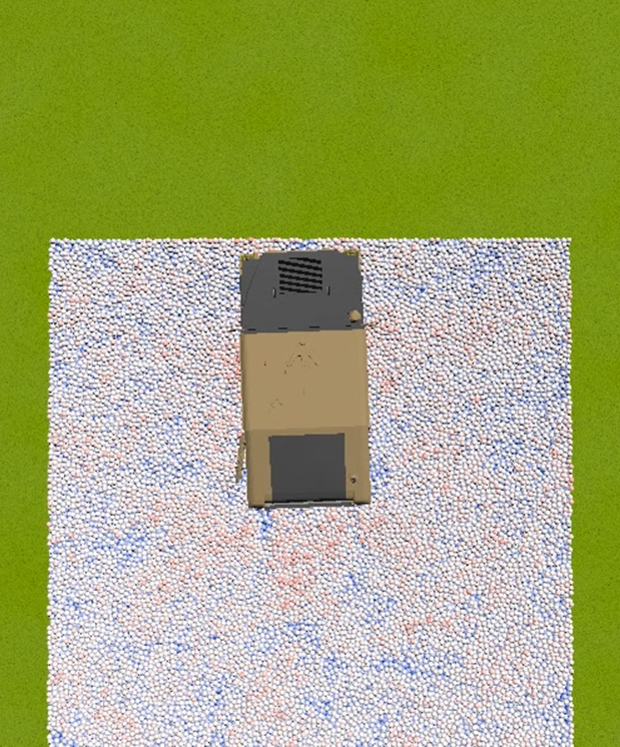
\includegraphics[width=\textwidth]{Figs/toRelocate.png}
		\caption{{\small Vehicle Approaches front wall just before relocation algorithm triggered}}   
		\label{fig:pre_relocate}
	\end{subfigure}
	\hfill
	\begin{subfigure}[b]{0.49\columnwidth}
		\centering
		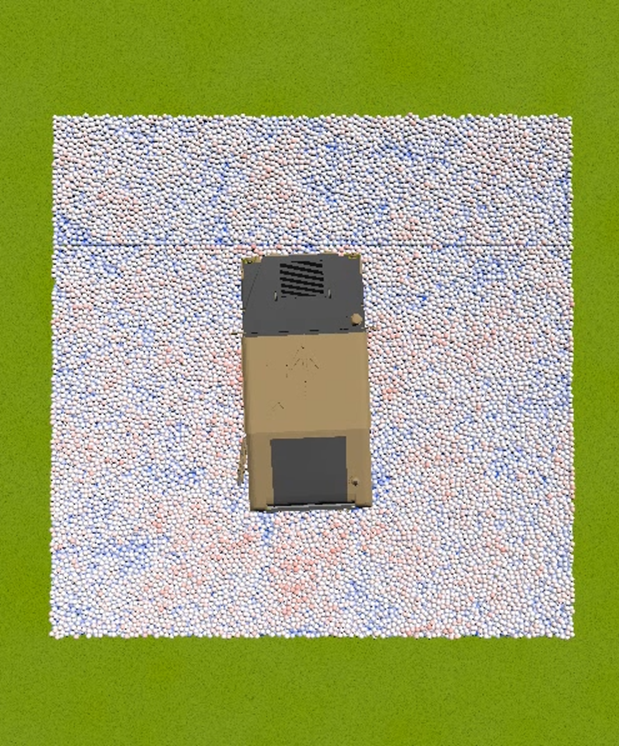
\includegraphics[width=\columnwidth]{Figs/justRelocated.png}
		\caption{\small Particles behind the vehicle are relocated to in front}   
		\label{fig:relocate}
	\end{subfigure}
	\caption{\small Granular relocation algorithm}
	\label{fig:relocationPics}
\end{figure}

For these simulations, the granular patch was maintained at a size of roughly $6.6$ by $6.6$ meters.  This number was assigned as two times the largest dimension of the vehicle.  The dimensions of the patch are not constant, however, since the patch expands in the direction of relocation by two times the largest particle radius every time the advancing wall is shifted.  This is done in order to avoid particle overlap, since the relocated particles are moved to a position that is shifted one largest particle radius ahead of the particles adjacent to the advancing wall.  After relocation, the walls of the granular patch are given a recovery velocity such that the granular patch regains its original dimensions in $0.1$ seconds.  This recovery time should be small relative to the duration of the simulations, and in general it will also depend on the velocity of the vehicle, since the granular patch should completely recover its dimensions between subsequent relocations.

To prevent the granular patch from colliding with the obstacles in the field, each body in the simulation is designated a family. Then within the simulation the user can designate which families collide with which other families. So the particles and their walls are all members of the same family. This family interacts only with the family containing the bodies of the HMMWV and not with the obstacle family. This framework allows the vehicle to approach and collide with the obstacles without the terrain actually experiencing that obstacle collision. Figure \ref{fig:relocationAroundObstacle} presents the vehicle on the granular patch maneuvering around an obstacle and though the terrain overlaps with the obstacle, no collision forces are calculated or applied between those families of bodies.

Within the granular patch, the granular terrain was modeled by $55,931$ uniform spherical particles, with a micro-scale inter-particle sliding friction coefficient of $\mu = 0.8$, and particle diameter of $0.1$~m.  Previous studies~\cite{fleischmannetalGEGE2014} have shown that 
a randomly packed assembly of as few as $3,000$ - $30,000$ uniform spheres will exhibit macro-scale bulk granular material yield behavior (due to inter-particle sliding) that closely matches the Lade-Duncan yield surface, which is a well-established yield criterion in the field of geomechanics, where the macro-scale friction angle $\phi$ for the bulk granular material can be determined as a function of the inter-particle friction coefficient $\mu$.

\begin{figure}
	\centering
	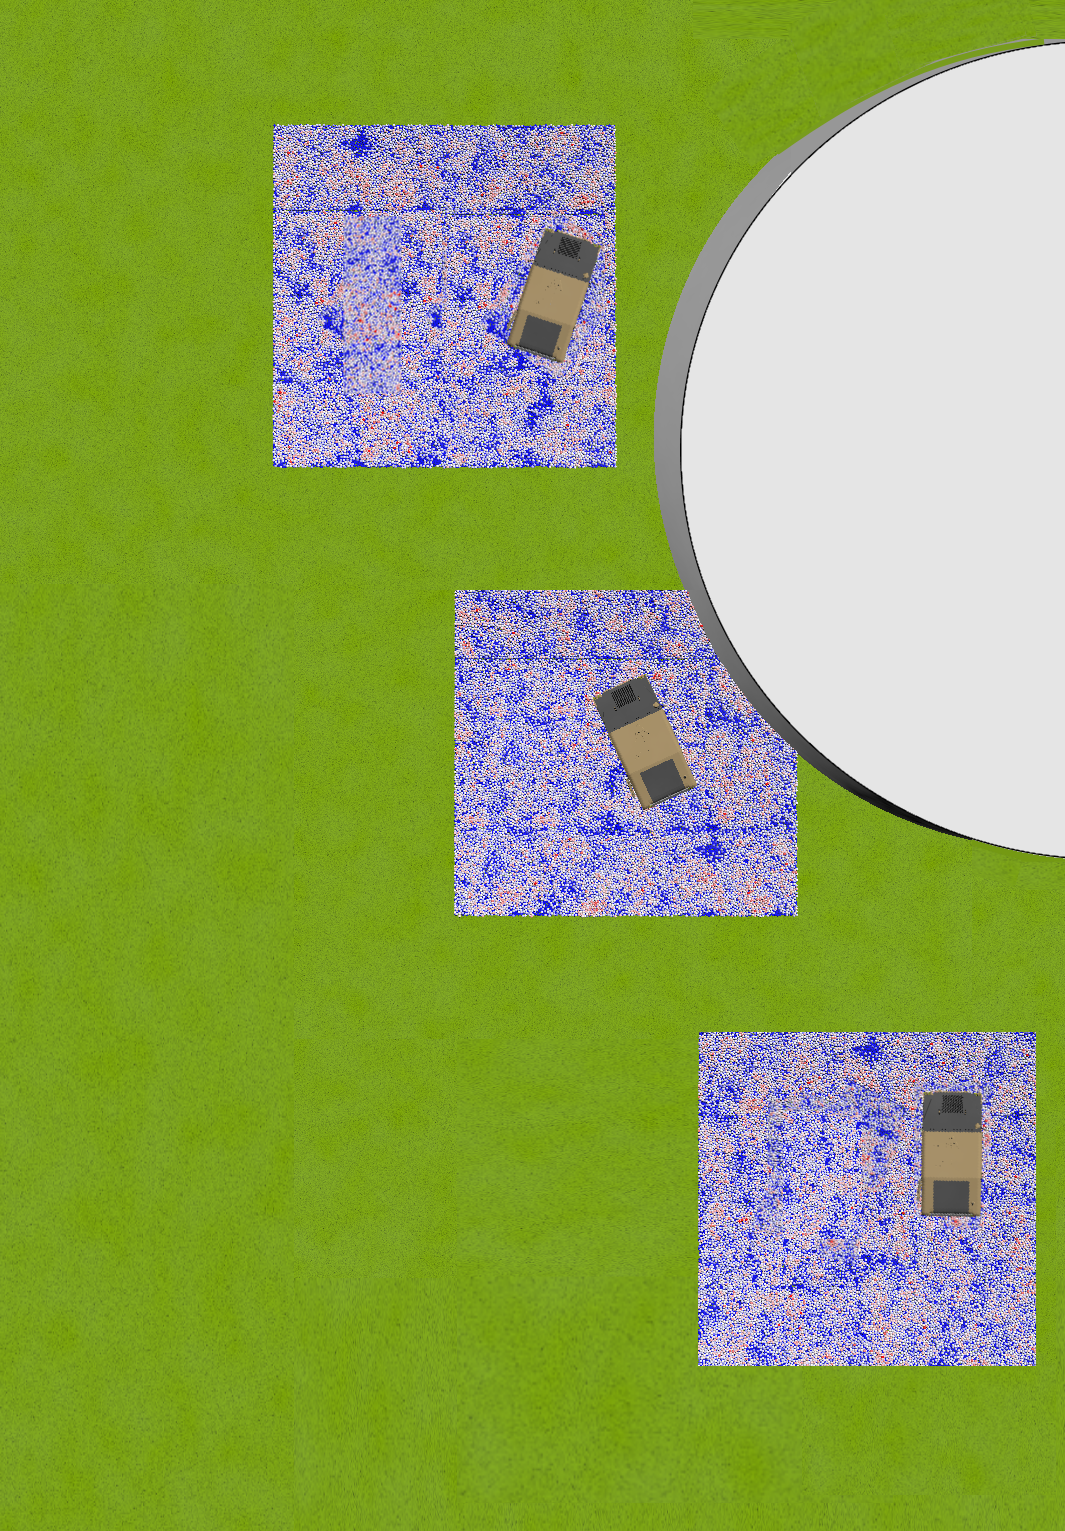
\includegraphics[width=0.8\columnwidth]{Figs/aroundObstacle.png}
	\caption{\small HMMWV navigating around obstacle, granular Patch does not collide with obstacles}
	\label{fig:relocationAroundObstacle}
\end{figure}

Figure \ref{fig:relocationPics} presents the single granular patch used for all granular simulations in the presented experiments of this thesis. The granular terrain is colored based on the particle global z location so that blue particles are low and red particles are high. An improved alternative to this single relocating granular patch was explored as well in an attempt to both speed up simulation runtimes and allow for simulation of smaller particles. The explored method was instead of using a single large granular patch underneath the vehicle, four individual independent and smaller granular patches are simulated underneath each of the vehicle wheels. This concept is visualized in Figure \ref{fig:4Patch}. This concept would allow for a much smaller number of particles to be simulated since resources again are not being wasted for particles sitting too far away from the wheels. Each smaller patch works the same as the large single granular patch where they are provided a location on the body to follow. As that point on the body moves a certain distance towards any of the walls holding the small patch of particles together, particles near the opposite wall are relocated to in front of the closer wall, the walls shift and compress to account for the patch growth to prevent particle overlaps during relocation. To prevent particles from one wheel patch from colliding with particles from another wheel patch, bodies are designated as members of a family depending on which patch they were generated in. Particles then only collide with the walls, particles, and wheel that are members of its own family. This allows patches to overlap without actually colliding with each other. 

This new concept was implemented in simulations to test its potential as a method for simulating granular terrain moving forward. Comparing the results of simulations using these four individual patches to those that used the single large patch, there were not significant differences in results or vehicle trajectories. The individual patches method even allowed for simulations with particles of diameter $0.05$~m without sacrificing larger amounts of time to perform these simulations. One note that supports the use of larger particles was even by reducing the particle size by that large of a factor, there was no real difference in vehicle performance. However, a concern with using these smaller patches was that there was a much more significant boundary effect each relocation step due to the smaller distance between the tire contact patch and the walls containing the particles. Figure \ref{fig:4Patch} presents a visualization of the four independent relocating patches explored. This concept shows promise but for consistency and more confidence in the fidelity of the simulation results, all recorded and presented simulations in this study use the single large relocating patch. The independent patches are considered for future research. 

\begin{figure}
	\centering
	\begin{subfigure}[b]{0.32\textwidth}
		\centering
		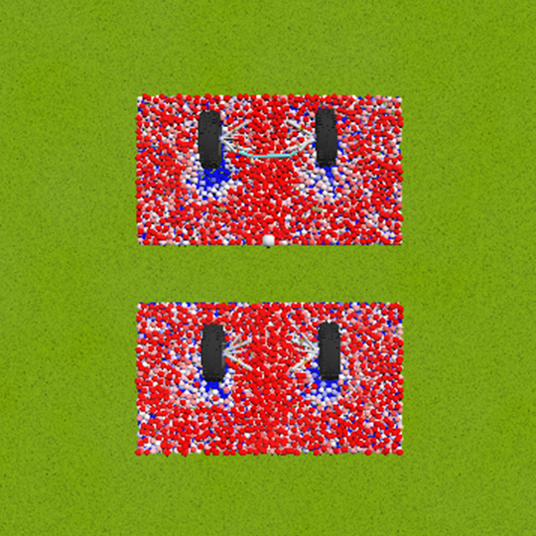
\includegraphics[width=\linewidth]{Figs/4patch1.png}
		\caption{\small Initial four relocating granular patches}   
		\label{fig:4PatchA}
	\end{subfigure}
	\hfill
	\begin{subfigure}[b]{0.32\textwidth}
		\centering
		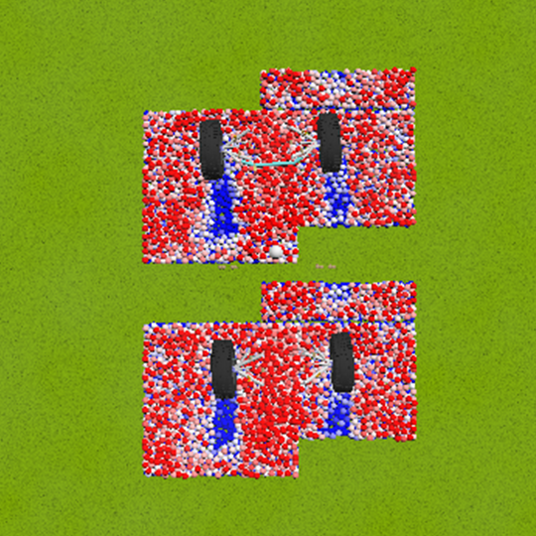
\includegraphics[width=\linewidth]{Figs/4patch2.png}
		\caption{\small Forward relocation step for the right wheel patches}   
		\label{fig:4PatchB}
	\end{subfigure}
	\hfill
	\begin{subfigure}[b]{0.32\textwidth}
		\centering
		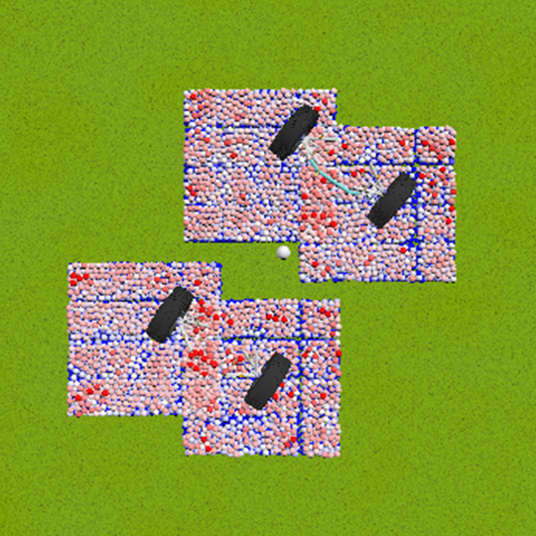
\includegraphics[width=\linewidth]{Figs/4patch3.png}
		\caption{\small Patches follow wheels as vehicle heading changes}   
		\label{fig:4PatchC}
	\end{subfigure}
	\caption{\small Independent four granular relocating patches explored to improve simulation speeds, HMMWV chassis not visualized}
	\label{fig:4Patch}
\end{figure}

Referring to Figure~10 of~\cite{fleischmannetalGEGE2014}, a randomly packed assembly of uniform spheres with an inter-particle friction coefficient of $\mu = 0.8$ will exhibit macro-scale yield behavior corresponding to a bulk granular material with a macro-scale friction angle between roughly $35^\circ \leq \phi \leq 40^\circ$ if particle rotation is allowed (6-DOF particles), or with a macro-scale friction angle between roughly $65^\circ \leq \phi \leq 70^\circ$ if particle rotation is prohibited (3-DOF particles).
%
Since the granular patch used in our simulations contains more than $50,000$ uniform spheres, we can reliably conclude that it is accurately modeling the yield behavior of a true granular material on the macro-scale: either with a macro-scale friction angle of $35^\circ-40^\circ$ if particle rotation is allowed, which is typical of a wide range of dry natural and crushed sands \cite{Cho&Dodds&Santamarina2006}; or with a macro-scale friction angle of $65^\circ-70^\circ$ if particle rotation is prohibited, which is typical of crushed or fragmented rock, such as railway track ballast \cite{Indraratnaetal1998}.

We note that in the case of the HMMWV, the vehicle tire width is equal to only approximately $2.5$ particle diameters in the granular patch.  This is less than ideal.  However, a more suited value of $10$ particle diameters per tire width would increase the number of particles in the granular patch to more than $3$ million, which would result in prohibitively slow simulations, particularly for events corresponding to physical time durations on the order of $10$ seconds or more.

\section{Hardware and Materials}\label{s:Hardware}

The simulations throughout this research were performed on a Quantum TXR430-512R computer with Scientific Linux 7.2 installed as the primary operating system and an Ubuntu 16.04 virtual machine. The specifications of the computer are outlined in Table \ref{t:galerkin}. MATLAB 2015b was used to generate all plots in a post-processing script and determine evaluation metrics from each test case. POVRAY was used to generate visualizations of the performed simulations. Due to the long runtimes of each granular simulation, real-time visualization is not possible or necessary. Therefore, visualization with POVRAY is used. Simulations output large POVRAY data files that describe the body locations, sizes, and orientations at each time step. A set of scripts in Python 2.7 were developed to generate images from the POVRAY output data files and then stitch the images together to create a 60 fps video with a prescribed camera angle. The user could define using the scripts the location and orientation of the camera, what point the camera should look at, and if the camera should follow the vehicle throughout the video. This tool allows for simple and effective development of videos and images as a post-processing method. Overall, all work will be accomplished using this computer and resources accessible on this computer. This computer outlined below is designed to run simulations with large amounts of bodies in a quick efficient manner.

\begin{table}
\begin{tabularx}{\textwidth}{|>{\setlength\hsize{0.7\hsize}\setlength\linewidth{\hsize}}X|>{\setlength\hsize{1.0\hsize}\setlength\linewidth{\hsize}}X|>{\setlength\hsize{1.8\hsize}\setlength\linewidth{\hsize}}X|>{\setlength\hsize{0.5\hsize}\setlength\linewidth{\hsize}}X|}
\hline
\textbf{Identifier} & \textbf{Basic Information} & \textbf{Additional Information} & \textbf{Quantity}\\
\hline
\textbf{Architecture} &
Quantum TXR430-512R &
$\cdot$ Tower / 4U Convertable Chassis \newline
$\cdot$ Supports 2x E5-2600 v3 Processors \newline
$\cdot$ DDR4 Memory \newline
$\cdot$ Supports Up To 3x 5.25IN Bays \newline
$\cdot$ 8x 3.5IN Hot-Swap HDD Bays \newline
$\cdot$ Up To 4x Double-Width GPU \newline
$\cdot$ Up To 1TB DDR4 Memory \newline
$\cdot$ Dual Gigabit Ethernet LAN \newline
$\cdot$ 2000W Redundant Power Supplies
&
1 \\
\hline
\textbf{Processor} &
Intel Xeon E5-2687W v3 &
10C, 3.1 GHz 25M, Support DDR4-2133 &
2 \\
\hline
\textbf{Memory} &
32GB DDR4 &
2133MHz LR ECC LRDIMM &
8 \\
\hline
\textbf{Primary Storage} &
512 GB 2.5 SATA III &
Internal Solid State Drive (SSD) ** OS DRIVE ** &
1 \\
\hline
\textbf{Secondary Storage} &
1.8 TB SAS &
12Gb/s 2.5InternalHardDrive**RAID10** &
8 \\
\hline
\textbf{RAID Controller} &
LSI 9300 MegaRAID SAS 9361-8i (LSI00417) PCI &
$\cdot$ Express 3.0x8 Low Profile SATA/SAS \newline
$\cdot$ 1 GB Cache \newline
$\cdot$ High Performance Eight-Port 12 Gb/s RAIDController
&
1 \\
\hline
\textbf{RAID Cache} &
LSI LSICVM02 & 
(LSI00418) CacheVault Accessory Kit for 9361 Series) &
 \\
\hline
\textbf{GPU} &
Nvidia Tesla K80 &
24 GB GDDR5 384-bit PCI Express 3.0 - Passive Cooling &
3 \\
\hline
\textbf{GPU Cooling} &
Passive Cooling &
Passive GPU Kit for 4U 4GP USystem & 
1 \\
\hline
\textbf{Power} &
PC Smart UPS X 3000VA &
Rack/Tower LCD100-127V &
1 \\
\hline
\multicolumn{2}{|c|}{\multirow{2}{*}{\textbf{Internal Cabling}}} &
0.6m Internal Cable SFF8643 to x4 SATA HDD (mini SASHD to SATA data port) &
2 \\
\hhline{~~--}
\multicolumn{2}{|c|}{} &
2.5" to 3.5" SATA/SAS6Gb SSD Hard Drive Converter / Adapter / Bracket &
9 \\
\hline
\multicolumn{2}{|c|}{\multirow{3}{*}{\textbf{Additional Components}}}  &
4U / Tower Conversion Kit / Rail Kit &
1 \\
\hhline{~~--}
\multicolumn{2}{|c|}{} &
Windows 8.1 Professional 64Bit &
1\\
\hhline{~~--}
\multicolumn{2}{|c|}{} & 
Samsung S24D300H 24IN LCD Monitor &
1 \\
\hline
\end{tabularx}
\caption{\small Hardware Components of Computer Used for Parallel Simulations}
\label{t:galerkin}
\end{table}

%% ============================================================

\chapter{FIRST EXPERIMENTAL RESULTS AND DISCUSSION}\label{c:results}

\begin{figure}
	\centering
	\begin{subfigure}[b]{0.49\columnwidth}
		\centering
		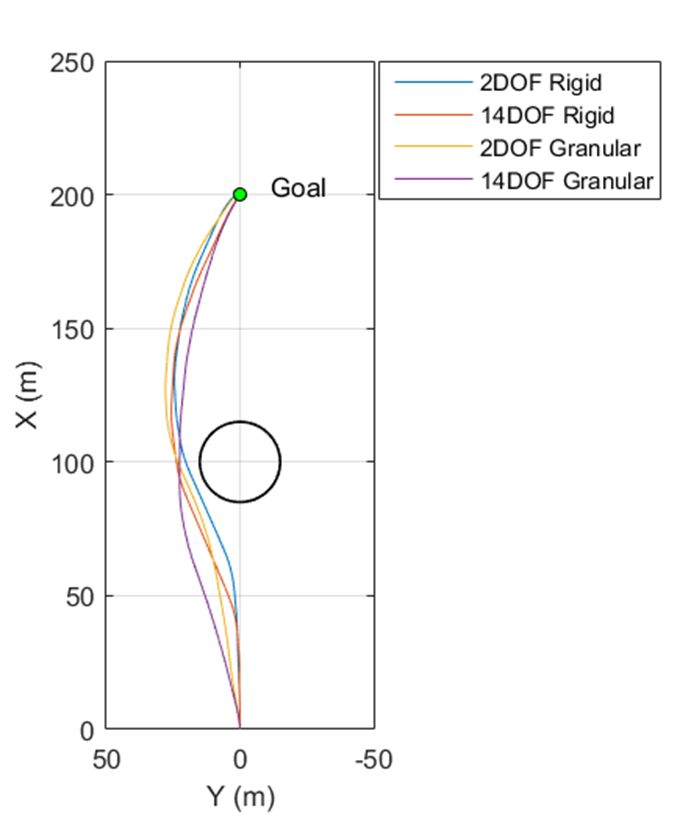
\includegraphics[height=\columnwidth]{Figs/ObstacleField1Trajectories.png}
		\caption{{\small Vehicle trajectories.}}   
		\label{fig:ObstacleField1Trajectories}
	\end{subfigure}
	\hfill
	\begin{subfigure}[b]{0.49\columnwidth}
		\centering
		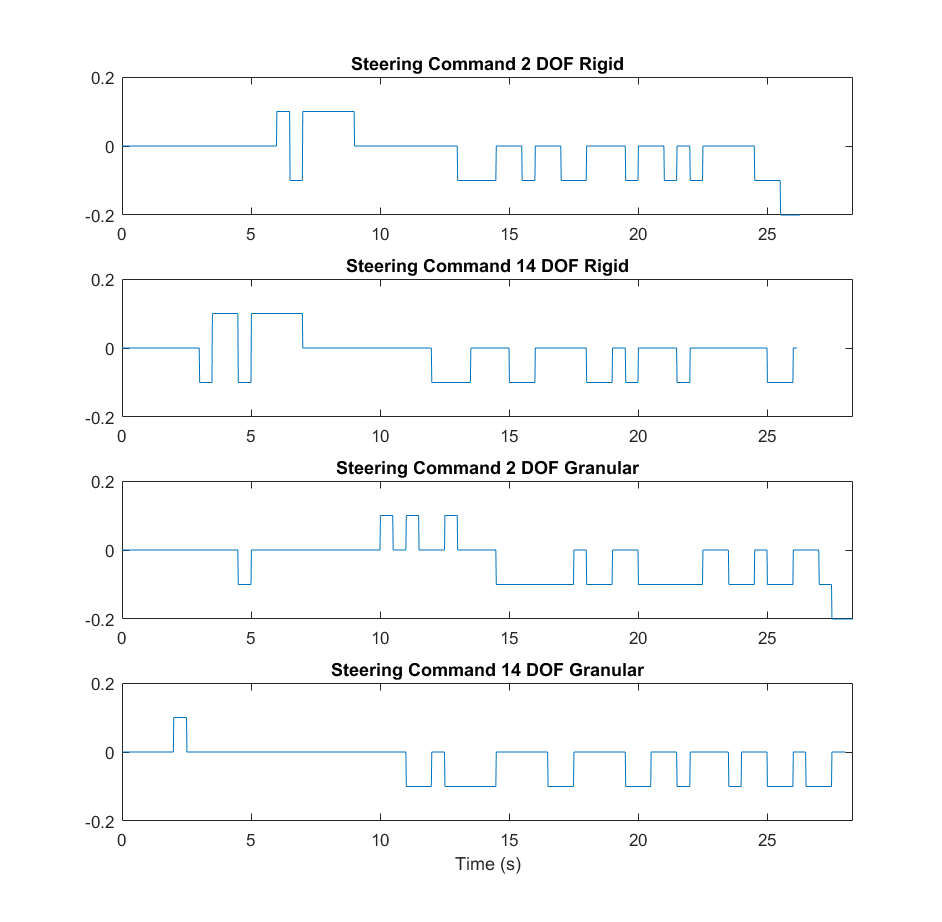
\includegraphics[width=\columnwidth]{Figs/SteeringCommandsField1.png}
		\caption{\small Steering commands.}   
		\label{fig:SteeringCommandsField1}
	\end{subfigure}
	\caption{\small Experiment 1 Test results on obstacle field 1}
	\label{fig:Obst1TestData}
\end{figure}

\begin{figure}
	\centering
	\begin{subfigure}[b]{0.49\columnwidth}
		\centering
		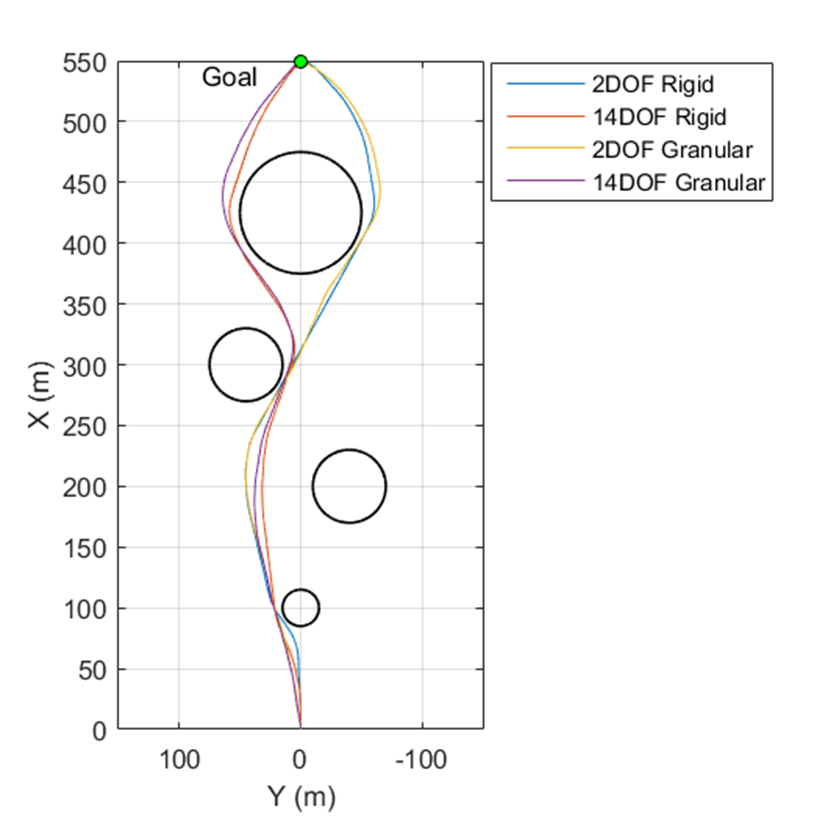
\includegraphics[height=\columnwidth]{Figs/ObstacleField2Trajectories.png}
		\caption{{\small Vehicle trajectories.}}   
		\label{fig:ObstacleField2Trajectories}
	\end{subfigure}
	\hfill
	\begin{subfigure}[b]{0.49\columnwidth}
		\centering
		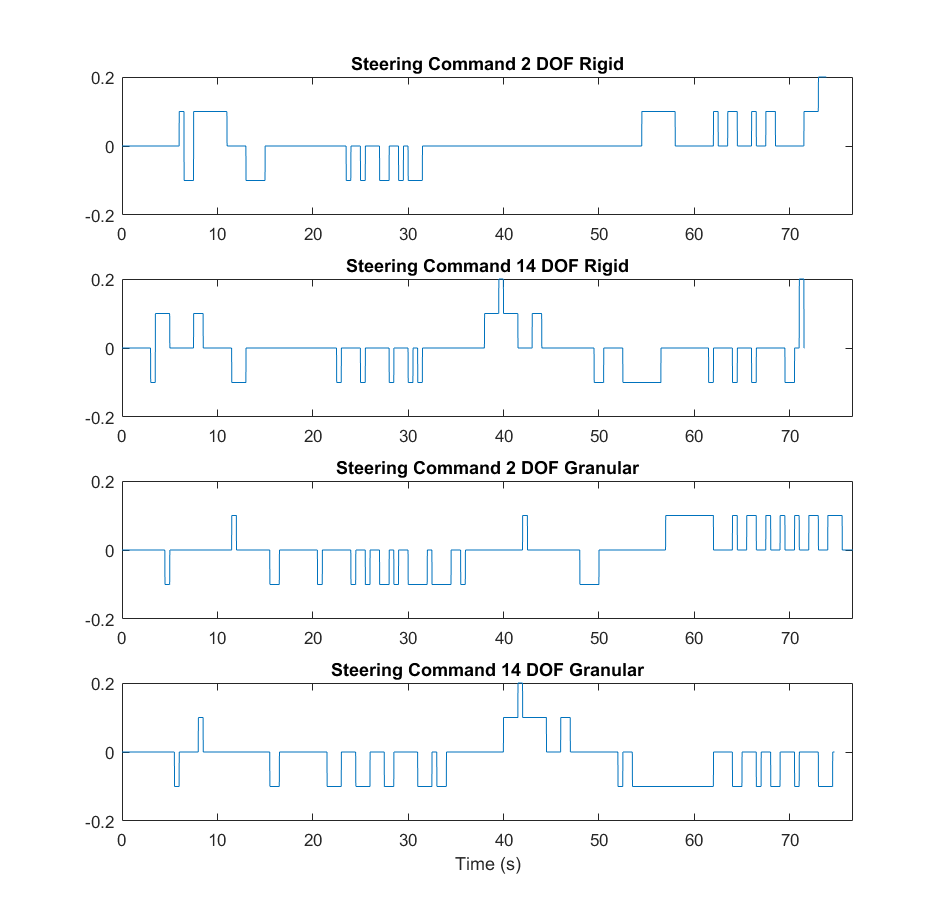
\includegraphics[width=\columnwidth]{Figs/SteeringCommandsField2.png}
		\caption{\small Steering commands.}   
		\label{fig:SteeringCommandsField2}
	\end{subfigure}
	\caption{\small Experiment 1 Test results on obstacle field 2}
	\label{fig:Obst2TestData}
\end{figure}

\begin{table}
		\centering
\begin{tabular}{ ||p{6cm}|p{1.8cm}|p{1.8cm}|p{1.8cm}|p{1.8cm}||  }
		\hline
		Test Number & 1 & 2 & 3 & 4\\
		\hline
		Controller Model & 2-DOF & 14-DOF & 2-DOF & 14-DOF\\
		\hline
		Terrain & Rigid & Rigid & Granular & Granular\\
		\hline
		Time to Target (s)  & 26.67 & 26.15 & 28.32 & 28.03\\ 
		\hline
		Minimum Obstacle Distance (m) & 0.897 & 5.462 & 3.491 & 4.721\\
		\hline
		Controller Effort & 0.0340 & 0.0340 & 0.0340 & 0.0306\\
		\hline
		Max. Lateral Acceleration (m/s$^{2}$)& 2.78 & 1.57 & 2.47 & 2.33 \\
		\hline
		Avg. Lateral Acceleration (m/s$^{2}$) &0.54 & 0.51 & 0.55 & 0.46\\
		\hline
\end{tabular}
\caption{Experiment 1 Test Evaluation Metrics Summary on Obstacle Field 1}
\label{t:EvalMetricsObst1}
\end{table}

\begin{table}
		\centering
\begin{tabular}{ ||p{6cm}|p{1.8cm}|p{1.8cm}|p{1.8cm}|p{1.8cm}||  }
		\hline
		Test Number & 1 & 2 & 3 & 4\\
		\hline
		Controller Model & 2-DOF & 14-DOF & 2-DOF & 14-DOF\\
		\hline
		Terrain & Rigid & Rigid & Granular & Granular\\
		\hline
		Time to Target (s)  & 73.85 & 71.55 & 76.64 & 74.70\\ 
		\hline
		Minimum Obstacle Distance (m) & 0.331 & 2.599 & 1.083 & 1.152\\
		\hline
		Controller Effort & 0.0510 & 0.0680 & 0.0714 & 0.0612\\
		\hline
		Max. Lateral Acceleration (m/s$^{2}$)& 2.92 & 2.51 & 2.55 & 2.45 \\
		\hline
		Avg. Lateral Acceleration (m/s$^{2}$) & 0.41 & 0.43 & 0.53 & 0.58\\
		\hline
\end{tabular}
\caption{Experiment 1 Test Evaluation Metrics Summary on Obstacle Field 2}
\label{t:EvalMetricsObst2}
\end{table}

This section summarizes the results of the four tests listed in Table~\ref{t:TestMatrix}. The trajectories for the four performed tests are presented in Figures~\ref{fig:ObstacleField1Trajectories} and \ref{fig:ObstacleField2Trajectories}, for obstacle fields 1 and 2, respectively. The associated steering commands generated by the controller are presented in Figures~\ref{fig:SteeringCommandsField1} and \ref{fig:SteeringCommandsField2}. The results of this first experiment are published in \cite{GVSETS2017}.

The evaluation metrics for each test, as defined in Section~\ref{s:Metrics}, are tabulated for each obstacle field in Tables~\ref{t:EvalMetricsObst1} and \ref{t:EvalMetricsObst2}. 

\section{Influence of model fidelity}

Assessing the effect of internal vehicle model fidelity on controller performance when the vehicle navigates on rigid terrain (comparison of tests 1 and 2), we make the following observations:
\begin{itemize}
\item the 14-DOF model leads to marginally faster travel to the target location;
\item the 2-DOF model leads to trajectories with lower obstacle clearance;
\item the two models result in the same controller effort on the first obstacle course; however, the higher-fidelity 14-DOF model requires 33\% more controller effort on the second obstacle course, a consequence of its decision of performing a course change to negotiate the last obstacle;
\item the two models result in approximately the same number of command changes on both obstacle courses;
\item the 14-DOF model results in lower maximum lateral accelerations.
\end{itemize}

Overall, while the higher-fidelity internal model leads to marginally better performance, the 2-DOF model is perfectly suitable for use in MPC-based local obstacle avoidance on rigid terrain at non-extreme speeds, as it can safely navigate the vehicle to its end goal. These results support the findings and conclusions in~\cite{ModelFidelity2016} even though a different AGV is considered here.

A similar comparison can be made for the case of obstacle avoidance on granular terrain (tests 3 and 4).  As on rigid terrain, the higher fidelity model leads to faster travel to the end goal, larger clearances to the obstacles, and lower maximum lateral accelerations.  However, on granular terrain, the controller effort required by using the 14-DOF model is always lower than that required by the 2-DOF model.  We again conclude that using a higher-fidelity internal controller model leads to overall marginally better performance.

The 2-DOF and 14-DOF internal vehicle models were derived using rigid ground assumptions, yet they are still capable of successfully and safely navigating the simulated vehicle through an obstacle field on granular terrain. The monitored metrics indicate a slight drop in controller performance when using the 2-DOF model. However, these gains are outweighed by the benefits, in terms of required computational effort, offered by implementing the lower-fidelity 2-DOF model. 

\section{Influence of terrain type}

Turning next to evaluating the 14-DOF internal controller model when navigating on rigid versus granular terrain (comparison of tests 2 and 4), we draw the following conclusions:
\begin{itemize}
\item on both obstacle courses, the target can be reached faster when navigating on rigid terrain;
\item the resulting trajectories are slightly closer to the obstacles when navigating on granular terrain;
\item the required controller effort is lower when navigating on granular terrain;
\item the maximum lateral accelerations are similar on both types of terrain.
\end{itemize}

A similar analysis can be performed on the 2-DOF model when used to control a vehicle on either rigid or granular terrain (comparison of tests 1 and 3). Unlike the 14-DOF model, the simpler 2-DOF model does a better job of approaching the obstacles more closely when controlling a vehicle on rigid rather than on granular terrain. Related to this, the controller effort on rigid terrain (test 1) is lower than that required on granular terrain (test 3). 


The forces the vehicle experiences from driving on granular terrain can be much different than forces on simple rigid ground. Examining Figures~\ref{fig:ObstacleField1Trajectories} and \ref{fig:ObstacleField2Trajectories}, the vehicle navigating on granular terrain does not turn as sharply for a given steering command as the vehicle does on rigid ground terrain. To understand the different behavior between a vehicle driving on rigid and granular terrain, a parametric study should be performed analyzing the vehicle driving on a variety of granular terrains with different granular parameters. 

Tests 3 and 4 were performed on granular terrain modeled as randomly packed uniform spheres with an inter-particle friction coefficient of $\mu = 0.8$, diameter of 0.1m, and a macro-scale friction angle roughly in the range $65^\circ \leq \phi \leq 70^\circ$, with particle rotation prohibited. This granular material resembles railway track ballast. These same tests were attempted on the the same randomly packed uniform spheres with particle rotation allowed resulting in a macro-scale friction angle between $35^\circ \leq \phi \leq 40^\circ$. This granular material resembles a dry sand. The results of this second set of tests on dry sand are not plotted or tabulated because the vehicle failed to move from the initial position. Instead, the vehicle spins its wheels in place at its initial location, making no progress forward as the wheels slowly dig themselves down into the granular terrain. However, this may be due to the too large diameter spheres used for this study for computational reasons. Generally the MPC LIDAR-based constant speed local obstacle avoidance controller used in this study is not yet appropriate for use on all granular terrains. There are situations where a combined speed and steering controller similar to that described in~\cite{SpeedSteer2015}, or even some new speed and steering controller which accounts for terrain parameters and mobility information to better predict vehicle movement, would be required. Neither of the models used in this first experiment, the rigid ground 2-DOF yaw plane model nor the rigid ground 14-DOF vehicle models, were appropriate for predicting vehicle behavior and performance on dry sand. Based on these findings, improvements were made to the 2-DOF and controller and are discussed below.

%% ============================================================

\chapter{IMPROVED VEHICLE MODEL ON GRANULAR MATERIAL}\label{c:improvedModel}
\section{Bekker/Wong Load Sinkage Relationship}\label{s:BekkerWong}

\begin{figure}
	\centering
	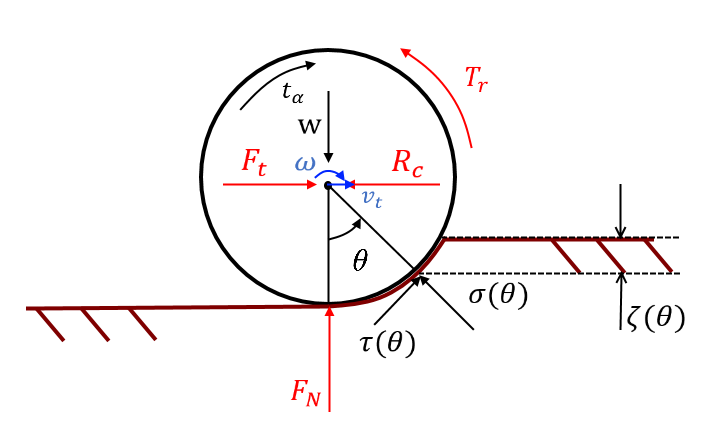
\includegraphics[width=0.8\columnwidth]{Figs/tireRolling.png}
	\caption{\small Terrain interactions on a single wheel on soft soil}  
	\label{fig:wheelTerrain}
\end{figure}

Often the interaction between a rigid tire and soft soil is modeled using terramechanics relations originating from the work of Bekker and Wong \cite{wong93}. Penetration tests were performed to simulate the contact area of a tire or track interacting with soft ground and the pressure $p$ and sinkage $z$ were measured for the array of experiments. Based on this experimental data, Bekker proposed the well known load-sinkage relationship in Equation \eqref{e:BekkerLoadSinkage} \cite{wong93}. $n$ is an exponent of deformation, $b$ is the width of the tire, $k_c$ is the cohesive modulus of deformation, and $k_\phi$ is the frictional modulus of deformation.
%
\begin{equation}\label{e:BekkerLoadSinkage}
p = \left(\frac{k_c}{b} + k_\phi\right)z^n
\end{equation}

If the normal stress is modeled anywhere along the wheel-terrain interface as Bekker proposed, then Equation \eqref{e:BekkerLoadSinkage} becomes Equation \eqref{e:modifiedNormal} where $\theta$ is defined in Figure \ref{fig:wheelTerrain}.
%
\begin{equation}\label{e:modifiedNormal}
\sigma\left(\theta\right) = \left(\frac{k_c}{b} + k_\phi\right)\zeta\left(\theta\right)^n
\end{equation}

Using terramechanics relations as in \cite{wong93}, the shear stress $\tau$ can then be determined along the wheel-terrain interface with Equation \eqref{e:shearStress} where $c$ is the terrain cohesion, $\phi$ is the internal friction angle of the granular terrain, $r$ is the wheel radius, $K$ is the shear deformation modulus, and $i$ is the wheel slip ratio defined in Equation \eqref{e:wheelSlipRatio}. $\omega$ is the angular speed of the wheel and $v_t$ is the speed of its center \cite{Ghotbi2016}. 
%
\begin{equation}\label{e:shearStress}
\tau\left(\theta\right) = [c+\sigma\left(\theta\right)tan\phi][1 - e^{-r[\theta_1 - \theta - \left(1-i\right)\left(sin\theta_1 - sin\theta\right)]/K}]
\end{equation}
\begin{equation}\label{e:wheelSlipRatio}
i = \frac{\left(r\omega-v_t \right)}{r \omega}
\end{equation}

\section{New Simplified Force Model}\label{s:NewForce}. 
The results in Chapter \ref{c:results} promote the need for a simple yet improved method of estimating the tire forces at the ground tire contact patch when a vehicle is operating on soft or granular terrain. A benefit to the Pacejka Magic Formula presented in Section \ref{s:Pacejka} is tire force calculation is backed by experimental data and the functions are shaped by a large number of experimentally determined parameters. However, the Magic Formula was derived for rigid ground applications only and does not succeed in estimating tire forces on granular terrain. The Magic Formula overestimates the lateral and longitudinal tire forces the vehicle experiences for any given slip angle as it does not take into account the shear strength of the soil. Therefore a simplified method of estimating the lateral tire forces at a tire ground contact patch was developed. This model is then used on the 2-DOF analytical vehicle model to estimate lateral tire forces and better predict vehicle trajectories on granular terrain.

\begin{figure}
	\centering
	\includegraphics[width=0.8\columnwidth]{Figs/forceComparison.png}
	\caption{\small Comparison of Magic Formula Lateral Force Prediction to New Force Model}  
	\label{fig:newForceComparison}
\end{figure}

Rather than using Equation \eqref{e:modifiedNormal} to calculate the normal stress at the tire ground contact patch, instead the normal load is calculated using Equations \eqref{e:FrontLoad} and \eqref{e:RearLoad}. Then the following assumptions are made. First, the tire ground contact patch is assumed to be square of side length $b$ which represents the width of the tire. Second, we assume a constant normal stress $\sigma$ throughout the contact patch such that the total force contribution from this normal stress is equal and opposite the normal load calculated in Equations \eqref{e:FrontLoad} and \eqref{e:RearLoad}. This leads to the simplified estimate of tire ground patch normal stress in Equation \eqref{e:simplifiedNormal}. Third, we assume the tangential stress along the tire contact patch to be constant as well. These assumptions lead to the simplification of \eqref{e:shearStress} and when we only consider the pure lateral slip case simplifies to Equation \eqref{e:simplifiedShear}.
%
\begin{equation}\label{e:simplifiedNormal}
\sigma = \frac{F_z}{b^2}
\end{equation}
\begin{equation}\label{e:simplifiedShear}
\tau = [c+\sigma tan\phi][1 - e^{-r[\frac{b}{r} - sin\left(\frac{b}{r}\right)]/K}]
\end{equation}

\begin{figure}
	\centering
	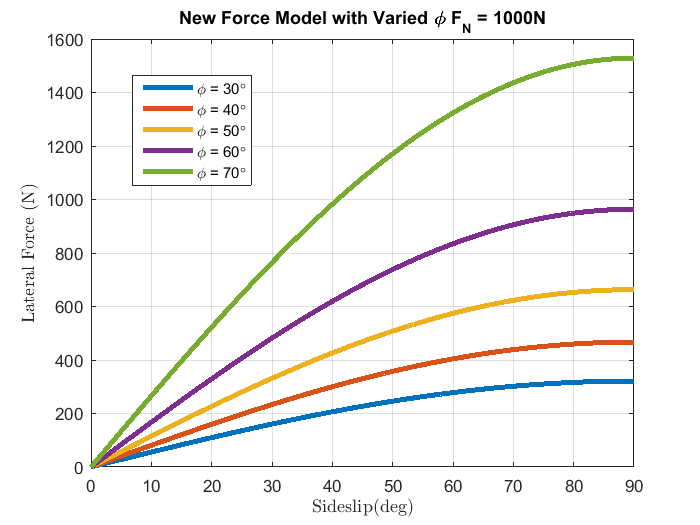
\includegraphics[width=0.8\columnwidth]{Figs/variedPhi.png}
	\caption{\small Effect of varying internal friction angle $\phi$ on lateral force prediction}  
	\label{fig:newForceComparison}
\end{figure}

Using the simplified constant stress relations and trigonometry, the lateral force is then calculated using Equation \eqref{e:newLatForce}. Though this development is the result of a handful of simplifying assumptions, the results of the formulation make sense. A comparison between the force prediction as a function of slip as predicted by the Magic Formula is compared to this new force model prediction in Figure \ref{fig:newForceComparison}. Intuitively one would expect these sorts of results because on granular terrain the tire ground contact patch is subject to a much more limited shear strength than a tire operating on rigid ground. This new force model then takes into account the cohesion and internal friction angle of the granular terrain in a meaningful way. The new model predicts higher lateral forces when a more cohesive soil or terrain with higher friction angle is used and vice versa. 
%
\begin{equation}\label{e:newLatForce}
F_y = -\tau b^2 sin\left(\alpha\right)
\end{equation}

\section{Open Loop Comparisons}\label{s:OpenLoop}

To justify that the new force model better models the lateral ground interaction force between a tire and granular terrain, a set of open loop simulations were performed. In these simulations, the HMMWV was initialized at rest, quickly accelerated to 8.3 m/s, and continued at this speed until the simulation has run for 10 seconds. Then the vehicle undergoes the steering sequence presented in Figure \ref{fig:openSteer} which consists of the vehicle steering left with a steering angle of 10 degrees for 5 seconds followed by steering right at a steering angle of -10 degrees for another 5 seconds. In this open loop test we are only interested in the vehicle's trajectory for the last 10 seconds of the simulation so only this time frame is considered and shown in plots.

Figure \ref{fig:openLoopmu} presents the resulting trajectories of 7 different open loop simulations run with this steering sequence with the parameters just discussed. One simulation was run on rigid flat ground while the other 6 were run on granular terrain consisting of non-rotating particles of inter-particle friction coefficients varying from $\mu$=0.66 to $\mu$=0.9. Lower values of $\mu$ were considered and tested, but these simulations resulted in the vehicle simply initializing and remaining stuck at the location where it started, constantly spinning its tires without making any forward progress. From these results it is shown that a vehicle operating on granular terrain will steer less sharply than the same vehicle operating on rigid ground undergoing the same steering sequence at the same speed. From these simulations we see there are clear differences in how a vehicle performs on rigid ground versus on granular terrain and this difference needs to be accounted for when attempting to model vehicle dynamic performance using simplified analytical equations. 

\begin{figure}
	\centering
	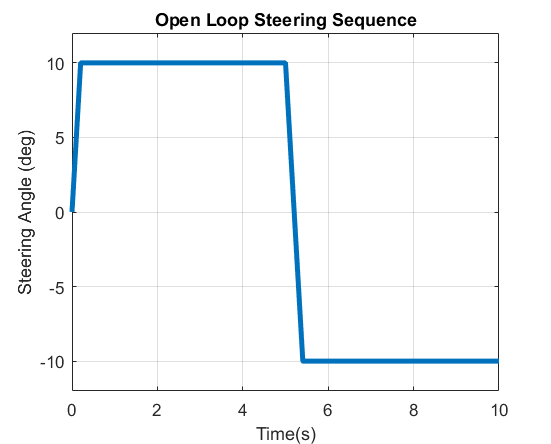
\includegraphics[width=0.8\columnwidth]{Figs/openLoopSteer.png}
	\caption{\small Steering Sequence used for Open Loop Simulations}  
	\label{fig:openSteer}
\end{figure}

\begin{figure}
	\centering
	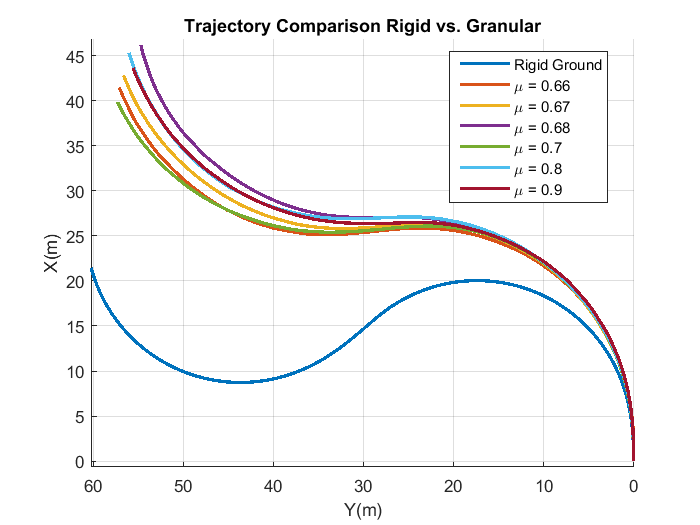
\includegraphics[width=0.8\columnwidth]{Figs/trajectoryComparison_png.png}
	\caption{\small Open Loop Trajectory of HMMWV over non-rotating granular terrains with different inter-particle friction coefficients $\mu$}  
	\label{fig:openLoopmu}
\end{figure}

\begin{figure}
	\centering
	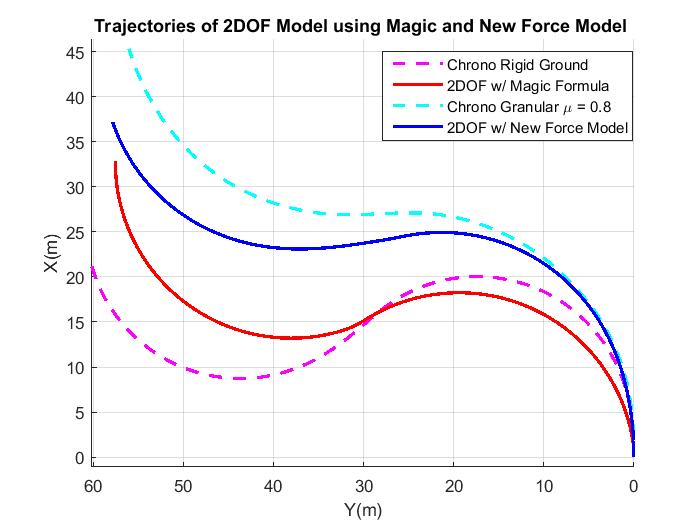
\includegraphics[width=0.8\columnwidth]{Figs/MagicvsNew.png}
	\caption{\small Comparison of Trajectory Predicted by 2-DOF model using the Magic Formula to estimate Tire Forces and the 2-DOF model using the new simplified force model}  
	\label{fig:MagicvsNew}
\end{figure}

The new force model developed in the previous section seeks to address this difference in vehicle performance based on terrain type. To confirm the new force model does a better job of modeling the lateral force experienced by a tire at the ground tire contact patch, two more open loop simulations were performed. Here the 2-DOF analytical yaw plane vehicle model was simulated for 10 seconds while undergoing the same steering sequence shown in Figure \ref{fig:openSteer}. In one simulation, the 2-DOF model uses the Pacejka Magic Formula to estimate lateral tire forces experienced by the vehicle. The second simulation uses the new force model to estimate the lateral tire forces experienced by the vehicle. These simulation trajectories are presented in Figure \ref{fig:MagicvsNew} along with the {\CHRONO} open loop simulation trajectories on rigid ground and non-rotating granular terrain with $\mu$=0.8. The 2-DOF vehicle model using the new force model to predict tire forces matches the {\CHRONO} simulation on granular terrain much more closely than the 2-DOF model using the Magic formula. Instead the 2-DOF model with the Magic Formula matches the {\CHRONO} simulation on rigid ground much better. Even though the results in Chapter \ref{c:results} show the controlled HMMWV was still able to successfully navigate to a target location while avoiding obstacles on granular terrain, there was a clear model mismatch between the internal vehicle controller model and the actual plant vehicle. The 2-DOF model using the Pacejka Magic Formula was overestimating the lateral tire forces because it did not take into account the granular terrain. This new force model does account for the granular terrain parameters and based on Figure \ref{fig:MagicvsNew} does a better job of predicting vehicle trajectories on granular terrain. 

%% ============================================================

\chapter{SECOND EXPERIMENTAL RESULTS TO TEST IMPROVED VEHICLE MODEL}\label{c:Exp2}

\section{Experimental Setup}\label{s:ExpSetup2}

\begin{table}
\begin{center}
	\begin{tabular}{||c |c | c | c||} 
		\hline
		Test  & Obstacle & Terrain  & Controller Vehicle \\
		Number &  Field & Type & and Force Model\\ [0.5ex] 	
		\hline\hline
		1 & 1 & Granular & 2-DOF Magic\\ 
		\hline
		2 & 2 & Granular & 2-DOF Magic\\
		\hline
		3 & 1 & Granular & 2-DOF New Model\\
		\hline
		4 & 2 & Granular & 2-DOF New Model\\
		\hline
	\end{tabular}
\end{center}
\caption{Compared Simulations for Second Experiment}
\label{t:TestMatrix2}
\end{table}

Another set of simulations were performed outlined in Table \ref{t:TestMatrix2}. This experiment consisted of four simulations on the same two obstacle fields as the previous experiment. Two analytical controller models are considered for this experiment, namely the 2-DOF model using the Pacejka Magic Formula to estimate lateral tire forces on the tires and another 2-DOF yaw plane vehicle model using the newly developed force model to estimate lateral tire forces. As was shown in Section \ref{s:OpenLoop}, open loop simulations enforced that this 2-DOF vehicle model with the new force model does a better job of predicting vehicle trajectories on granular terrain than the previously used Magic Formula 2-DOF models. The same evaluation metrics summarized in Section \ref{s:Metrics} are used in this experiment to compare simulation runs and determine which controller actually worked best. However, we are primarily concerned with the Time to Target evaluation metric in this experiment and therefore this will be the most influential factor in determining which controller worked best. 

\section{Results}\label{s:Results2}

\begin{figure}
	\centering
	\begin{subfigure}[b]{0.49\columnwidth}
		\centering
		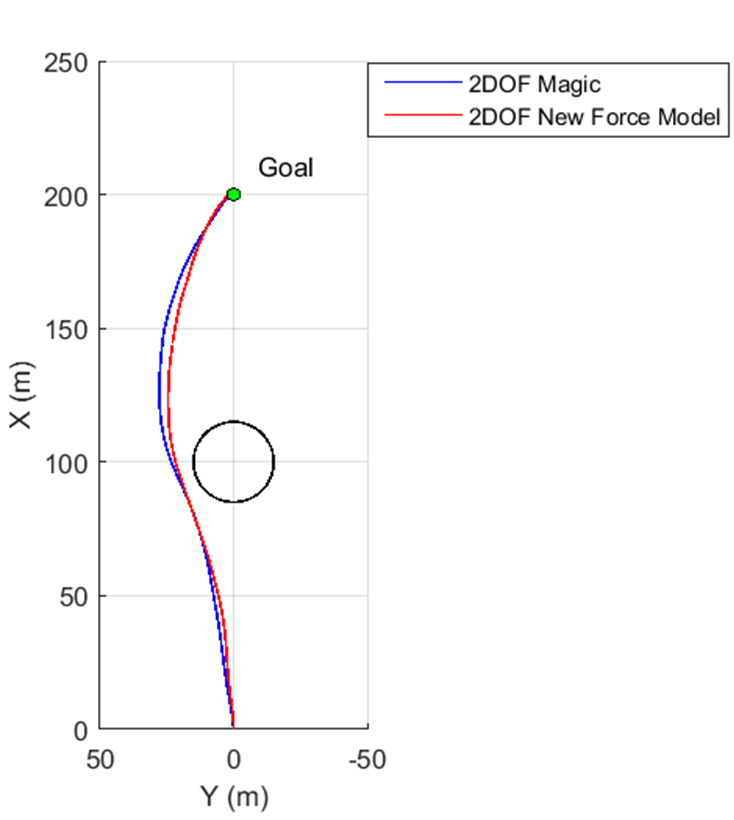
\includegraphics[height=\columnwidth]{Figs/Field1MagicvBekkerTrajectories_cropped.png}
		\caption{{\small Vehicle trajectories.}}   
		\label{fig:ObstacleField1TrajectoriesExp2}
	\end{subfigure}
	\hfill
	\begin{subfigure}[b]{0.49\columnwidth}
		\centering
		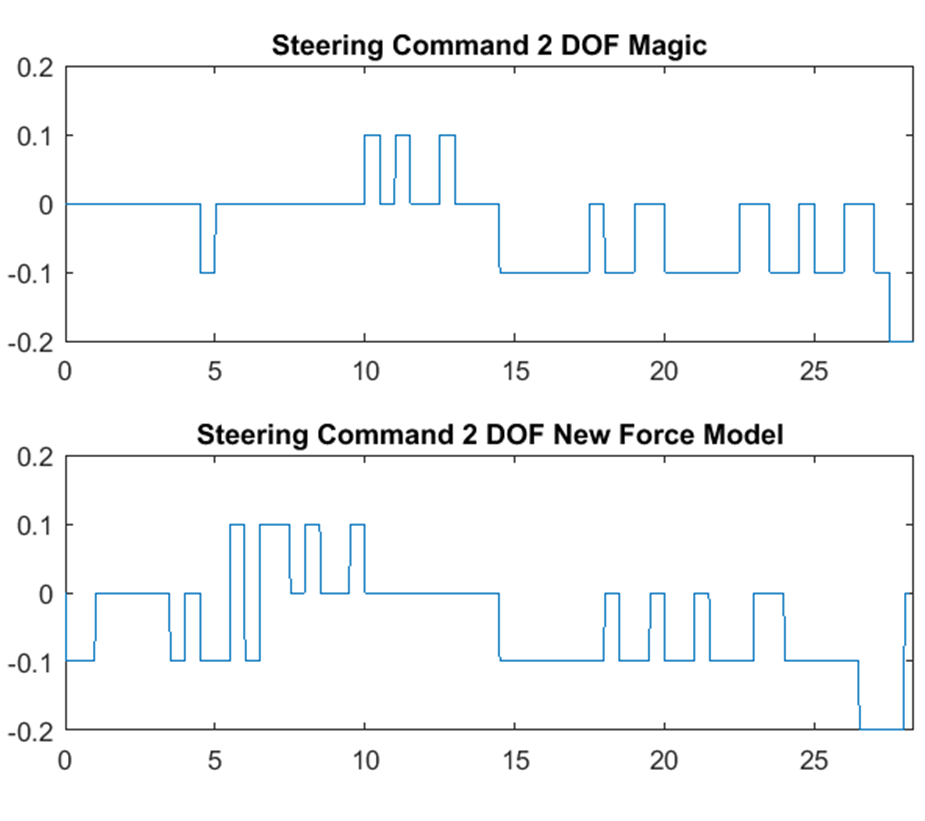
\includegraphics[width=\columnwidth]{Figs/Field1MagicvBekkerSteeringCommands_cropped.png}
		\caption{\small Steering commands.}   
		\label{fig:SteeringCommandsField1Exp2}
	\end{subfigure}
	\caption{\small Experiment 2 Test results on obstacle field 1}
	\label{fig:Obst1TestDataExp2}
\end{figure}

\begin{figure}
	\centering
	\begin{subfigure}[b]{0.49\columnwidth}
		\centering
		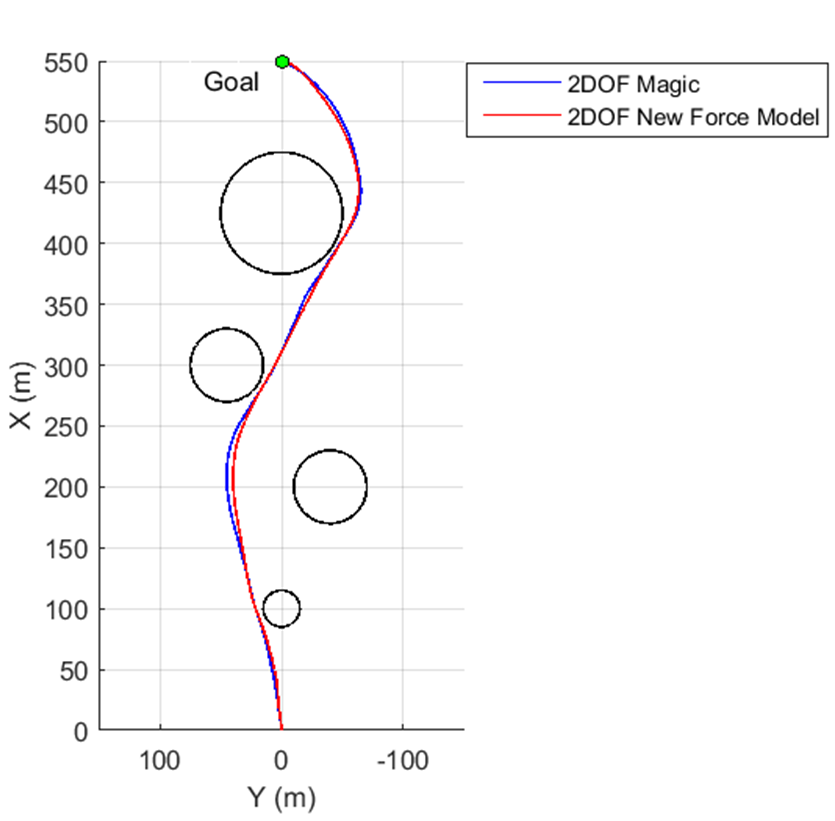
\includegraphics[height=\columnwidth]{Figs/Field2MagicvBekkerTrajectories_cropped.png}
		\caption{{\small Vehicle trajectories.}}   
		\label{fig:ObstacleField2TrajectoriesExp2}
	\end{subfigure}
	\hfill
	\begin{subfigure}[b]{0.49\columnwidth}
		\centering
		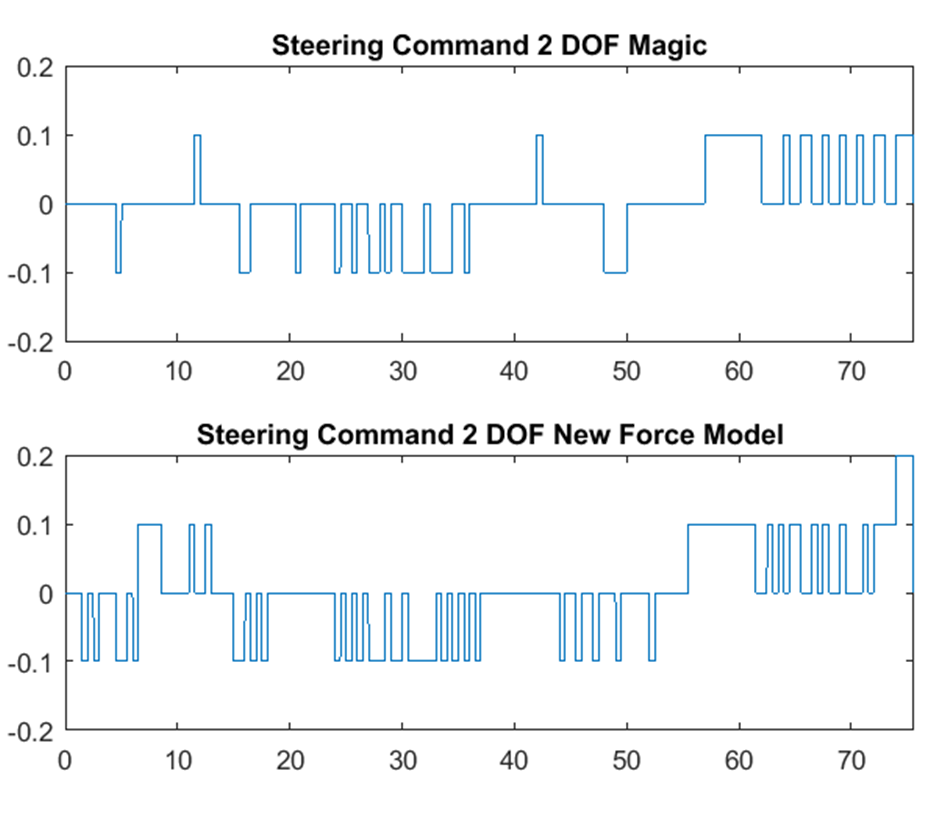
\includegraphics[width=\columnwidth]{Figs/Field2MagicvBekkerSteeringCommands_cropped.png}
		\caption{\small Steering commands.}   
		\label{fig:SteeringCommandsField2Exp2}
	\end{subfigure}
	\caption{\small Experiment 2 Test results on obstacle field 2}
	\label{fig:Obst2TestDataExp2}
\end{figure}

The trajectories for the four performed tests are presented in Figures~\ref{fig:ObstacleField1TrajectoriesExp2} and \ref{fig:ObstacleField2TrajectoriesExp2}, for obstacle fields 1 and 2, respectively. The associated steering commands generated by the controller are presented in Figures~\ref{fig:SteeringCommandsField1Exp2} and \ref{fig:SteeringCommandsField2Exp2}. The evaluation metrics for each test, as defined in Section~\ref{s:Metrics}, are tabulated for each obstacle field in Tables~\ref{t:EvalMetricsObst1Exp2} and \ref{t:EvalMetricsObst2Exp2}. 

\begin{table}
		\centering
\begin{tabular}{ ||p{6cm}|p{3.5cm}|p{3.5cm}||  }
		\hline
		Test Number & 1 & 3 \\
		\hline
		Controller Model & 2-DOF & 2-DOF \\
		\hline
		Terrain & Granular & Granular\\
		\hline
		Force Model & Magic Formula & New Force Model\\
		\hline
		Time to Target (s)  & 28.32 & 28.15 \\ 
		\hline
		Minimum Obstacle Distance (m) & 3.491 & 2.837 \\
		\hline
		Controller Effort & 0.0340 & 0.0381 \\
		\hline
		Max. Lateral Acceleration (m/s$^{2}$)& 2.47 & 2.69 \\
		\hline
		Avg. Lateral Acceleration (m/s$^{2}$) & 0.55 & 0.53 \\
		\hline
\end{tabular}
\caption{Experiment 2 Test Evaluation Metrics Summary on Obstacle Field 1}
\label{t:EvalMetricsObst1Exp2}
\end{table}

\begin{table}
		\centering
\begin{tabular}{ ||p{6cm}|p{3.5cm}|p{3.5cm}||  }
		\hline
		Test Number & 2 & 4 \\
		\hline
		Controller Model & 2-DOF & 2-DOF \\
		\hline
		Terrain & Granular & Granular\\
		\hline
		Force Model & Magic Formula & New Force Model\\
		\hline
		Time to Target (s)  & 76.64 & 75.58 \\ 
		\hline
		Minimum Obstacle Distance (m) & 1.083 & 1.440 \\
		\hline
		Controller Effort & 0.0714 & 0.0952 \\
		\hline
		Max. Lateral Acceleration (m/s$^{2}$)& 2.55 & 2.75 \\
		\hline
		Avg. Lateral Acceleration (m/s$^{2}$) & 0.53 & 0.51 \\
		\hline
\end{tabular}
\caption{Experiment 2 Test Evaluation Metrics Summary on Obstacle Field 2}
\label{t:EvalMetricsObst2Exp2}
\end{table}

From the results summarized in the plots and tables, the 2-DOF model using the new force model to predict lateral tire forces results in the HMMWV navigating to the target quicker than the 2-DOF controller using the Magic Formula to estimate tire forces. This improved performance is witnessed on both obstacle fields. On obstacle field 1, the new force 2-DOF model navigates closer to the single obstacle than the 2-DOF Magic model but this is just the opposite on obstacle field 2. On both obstacle fields, the controller effort of the new force 2-DOF model is slightly higher than the controller effort of the 2-DOF Magic controller. Finally, the average and lateral accelerations experienced by the vehicle when controlled by each different 2-DOF model are similar and the magnitude differences are negligible. 

Qualitatively examining the trajectories of all four tests, the trajectory of the 2-DOF new force model controller appears to be much smoother on both obstacle fields than its 2-DOF Magic controller counterpart. This is evident when looking at the runs on the first obstacle field. The 2-DOF Magic model commands result in the HMMWV taking a much wider turn followed my a more aggressive turning maneuver to reach the target position. However, when the vehicle is controlled by the 2-DOF model with the new force model, the HMMWV takes a more direct route to the target position and this improved performance is expressed in the decreased Time to Target. This difference is due to the Magic Model's overestimation of lateral tire forces that the HMMWV experiences. Since the 2-DOF vehicle model using the Magic formula estimates the vehicle can turn sharper at a given steering angle than the terrain actually allows, the predicted trajectories for any given steering angle are wrong and the HMMWV ends up changing its heading less than the controller predicts. This can also be seen comparing the trajectories on obstacle field 2. Both controllers command the HMMWV to follow similar trajectories, navigating the HMMWV in the same direction around all of the obstacles. Again though the 2-DOF new force model controller trajectory seems smoother of the two. The internal analytical vehicle model matches the plant vehicle better which leads to predicted trajectories that match the actual behavior of the HMMWV. These two facts combined lead to a better controlled HMMWV that navigates the the target quicker than if its trajectories were predicted using the 2-DOF Magic formula model. 

Overall based on the comparison of evaluation metrics and qualitative comparison of the trajectories, in this experiment the controller with the 2-DOF vehicle model using the new force model performed better than the controller using a 2-DOF model with the Magic formula. The trajectories of the controlled HMMWV are smoother and result in quicker Time to Target metrics. It is therefore possible to develop a tire force model which takes into account the soil parameters to estimate the lateral forces at the tire ground contact patch and use this new tire model to better predict vehicle trajectories in a MPC controller. In the future, this 2-DOF vehicle model with the new force model should be used or developed further to better control a wheeled vehicle on flat granular terrain of varying cohesive and shear strengths as well as inter-particle friction coefficients. 

%% ============================================================

\chapter{CONCLUSIONS}\label{c:conclusion}

In this study, using the multibody physics API {\CHRONO} a simulation has been developed of a HMMWV driving through a user specified obstacle field towards a defined target location. Within this simulation, a MPC LIDAR based local obstacle avoidance controller has been implemented to navigate the vehicle around obstacles as it encounters them. The controller itself uses a simplified analytical vehicle model to predict the actual controlled {\CHRONO} vehicle states within a finite prediction horizon in order to determine the optimal path and steering sequence forward from the current vehicle state. A method of simulating granular terrain for this large obstacle field was developed and implemented for this study. Two separate MPC Algorithms were developed initially, one that uses a 2-DOF vehicle model using the Pacejka Magic Formula as a tire model to predict {\CHRONO} vehicle states and a 14-DOF model to do the same. These two controllers were used to navigate a {\CHRONO} HMMWV through two obstacle courses on both rigid terrain and then on granular terrain. The results were compared to understand what if any improvements need to be made to the MPC LIDAR based local obstacle avoidance controller to successfully control a vehicle on granular terrain. 

As in \cite{ModelFidelity2016}, the controller with the 14-DOF internal vehicle model performs marginally better than the controller with the 2-DOF internal vehicle model in all situations. However, tests with the 2-DOF controller prove that this controller can still successfully navigate a vehicle through an obstacle field when the vehicle is moving at non-extreme speeds. Using the 2-DOF controller also allows for faster calculation of optimal steering sequences which is required for eventual real-time implementation. Both of the controllers navigated the vehicle worse on granular terrain than on rigid ground terrain, but this is expected since the internal vehicle controller models were derived using rigid ground assumptions. This study also highlights the complexities introduced to vehicle modeling when the terrain is no longer rigid. Looking at the vehicle trajectories and lateral accelerations on granular terrain, there are clear differences in tire ground interactions when the terrain is now granular. The terrain granular parameters affect the turning characteristics of the vehicle, acceleration abilities, and overall vehicle dynamic performance which is not control predictive with the currently used 2-DOF and 14-DOF analytical vehicle models. 

From the results of the first experiment, a new lateral tire force model was developed using common terramechanics relationships developed by Wong and Bekker. This new force model uses the cohesive strength and internal friction angle of the granular terrain to calculate the lateral forces experienced by a tire provided the current slip angle and wheel speed. From the first experiment, it was determined that though the 14-DOF internal vehicle model resulted in better controller performance, the complexity of this model made it undesirable for real-time implementation. Though the 2-DOF controller navigated to the target marginally slower, it still did succeed in reaching the target. Therefore the 2-DOF model was deemed desirable for future studies due to its success in reaching the target as well as the quicker runtime speeds necessary to determine an optimal path. For this reason then a second experiment was conducted using two different controllers. The first is the same controller from the first experiment consisting of an internal 2-DOF vehicle model using the Pacejka Magic Formula to predict vehicle trajectories. The second controller uses the 2-DOF vehicle model but with the new lateral force model to better predict trajectories on granular terrain. These controllers were tested on the same two obstacle fields from the first experiment but solely on a granular terrain resembling a stiff railroad ballast, the same granular terrain as from the first experiment. The new controller performed better than the old controller using the Magic formula to predict tire forces and this improvement is shown by a lower Time to Target as well as smoother trajectories with the second controller. This new intermediate analytical model is not as complex as the 14-DOF model but does take into account granular parameters such as the internal friction angle to result in more accurate vehicle trajectory predictions on granular terrain and ultimately a better controlled HMMWV. 

Each of the five objectives have been accomplished through the development and execution of the experiments described in this study. For clarification, a summary of each of the five objectives and how they were accomplished are presented as follows.

\begin{enumerate}
\item
Develop a robust simulation environment using {\CHRONO} to simulate granular terrain efficiently over large terrains without actually modeling every single particle over the large terrain. This was accomplished by leveraging the multibody and parallel computational abilities provided by {\CHRONO}. A novel relocating soil patch was developed to make simulation of a vehicle traversing large granular terrains possible without requiring months of runtime per experiment. 
\item
Study the performance of the MPC Controller on granular terrain as compared to that on rigid terrain. The results of this specific performance analysis are summarized in Chapter \ref{c:results}. These results enforced the need for more research into a better method of predicting tire forces at the tire ground patch in a simple manner. 
\item
Analyze the impact of fidelity of the internal controller model on speed and performance of the obstacle avoidance controller. These results are summarized in Chapter \ref{c:results} for Experiment 1. Overall similar conclusions were made to those drawn in \cite{ModelFidelity2016}. Namely, the controller using the more complex 14-DOF model resulted in marginally quicker Time to Target metrics than the 2-DOF controller model, but the increased complexity of the 14-DOF model increased controller runtimes making the 14-DOF model an undesirable choice for real-time implementation. The 2-DOF controller did still perform successfully and was chosen for more development to  improve its performance in Experiment 2. The 14-DOF model should be used to determine safety constraints to impose on a 2-DOF model used as the controller model. 
\item
Improve the controller for better performance on granular terrain. Chapter \ref{c:improvedModel} presents the development of this improved 2-DOF vehicle model which uses a newly developed lateral force model stemming from Bekker and Wong's terramechanics relations to more accurately predict vehicle trajectories on granular terrain. Chapter \ref{c:Exp2} presents the results of a second experiment run to confirm the newly developed vehicle model results in better controlled HMMWV performance.  
\item
Showcase the potential of controller testing in a high fidelity virtual test environment with {\CHRONO} to assist with initial control algorithm development before physical implementation for vehicular applications. All of the simulations and experiments from this study support and prove this objective. Using {\CHRONO} to create a virtual testing environment made it possible to quickly change aspects of the controller design to understand specific aspects of the control algorithm such as model fidelity or terrain's effect on controller performance. Testing the controller through simulation allowed for quicker and safer experiments than if one were to attempt to run each of these experiments in real life. Though the goal of these virtual experiments is to eventually prepare the controller for real life implementation and tests, these virtual tests should speed up the design process and make real life experiments that much more beneficial and meaningful to the design team. 
\end{enumerate}

Richard Hamming once said the purpose of computing is insight, not numbers \cite{NumMethods}. All mathematical models are an abstraction of reality, so what the user is interested in exploring or modeling should drive the complexity of the model. Detailed analysis of vehicle performance requires sophisticated high fidelity models often leveraging complex contact algorithms and sophisticated tire behavior representations. Control engineers make use of mathematical models to describe the dynamics of the system they are attempting to control. Linearizations, model simplifications, and other assumptions allow the controller to increase its speed while still describing the desired aspect of the system appropriately. This point is important when considering all of the research and work done to achieve the results of this study. Computer simulations can be extremely beneficial to the design process as long as the user has a strong understanding of the background, mathematical models, and methods that have driven the simulations. However, simulation simply cannot and more importantly should not replace all real life experimentation. No matter how complex a developer makes their simulation, it will still always be an abstraction of reality to some degree. However, it can be an extremely powerful tool in the design process, allowing a user to test core functionalities of their mechanical or controller design to gain insight towards how to improve their design. When used in this manner, virtual and real life experimentation can cooperatively contribute to quicker and more effective design processes. If more tests are run virtually then this saves money and time for the team that then runs physical tests on the most promising designs from virtual experimentation.  

This applies directly to all of the work and research performed in this study. This research has provided insight into the MPC LIDAR-based local obstacle avoidance controller. Due to this experiments outlined in this thesis, there is now a better understanding of how model fidelity and terrain affect the performance of this researched controller. From the insight gained from the first experiment, the controller and internal model were improved and tested virtually. The results of the second experiment emphasized that it is possible to develop a simplified vehicle model that predicts its lateral tire forces using simple terramechanics relations and allow the controlled vehicle to better navigate on granular terrain of varying cohesive strength and frictional properties. In these experiments, a high fidelity sophisticated multibody physics model of a HMMWV was used as the plant vehicle due to the goal of this simulation which is to analyze vehicle performance when controlled by different MPC controllers. Inside of the controller then, simplified analytical vehicle models are used which are another level of abstraction in order to quickly predict the trajectory of the simulated HMMWV based on terrain parameters. As simulation methods improve and computational speeds continue increasing, simulation's role in the design process will increase which can lower design costs and improve design speeds as well. 

\section{Future Work}\label{s:FutureWork}

The results of this study are promising. Since the 2-DOF controller is able to navigate the {\CHRONO} vehicle on this study's granular terrain, then there is some small set of granular terrain on which a 2-DOF model using the Magic formula is sufficient for predicting vehicle performance well enough to guide the vehicle successfully and safely to a target point. However, a new force model was developed using terramechanics relations to better approximate the lateral tire forces experienced by the 2-DOF vehicle model which results in better approximations of vehicle trajectories on granular terrain. This research opens up many opportunities and avenues for future research topics. This research lends itself to a variety of different parametric studies to understand how changing aspects of the terrain or controller affects the overall vehicle performance. For example, parametric studies examining controller performance on a wider array of granular terrains would allow for insight into how granular terrain parameters affect vehicle performance. In this research exhaustive search space was used to find an optimal solution. In the future though, a much quicker optimization method would be necessary to solve the optimal control problem each time step and ultimately implement the controller in real-time applications. 

A newer control algorithm could be developed all together with the goal of navigating a vehicle on all sorts of terrains. If instead of using a constant speed internal vehicle model and searching for an optimal steering sequence only, a controller could search for an optimal steering and acceleration input. If this were the case then the terrain parameters would impose constraints on how quickly a vehicle could actually accelerate on the terrain thus constraining the search space and resulting in a much smarter granular terrain navigation controller. 

Another avenue of research would be to explore improvements to the granular simulations developed in this study. To simulate granular terrain, in this study a novel relocating granular patch mechanism was developed that simulates a significant thickness of granular terrain underneath the vehicle at all times and relocates particles in front of the vehicle as it moves in any direction. This research would not have been feasible without the development of this mechanism, but as with any research topic there are further improvements that could help simulation speeds for these sorts of experiments. One possible improvement would be the implementation of periodic boundary conditions at the walls of the relocating patch to minimize any boundary effects at the tire ground contact patch. The independent four granular patches described in this thesis as well could be explored and tested further as a method to improve simulation speeds. That combined with periodic boundary conditions could potentially result in a quick and robust method for simulating granular terrain. 


\begin{figure}
	\centering
	\begin{subfigure}[b]{0.49\columnwidth}
		\centering
		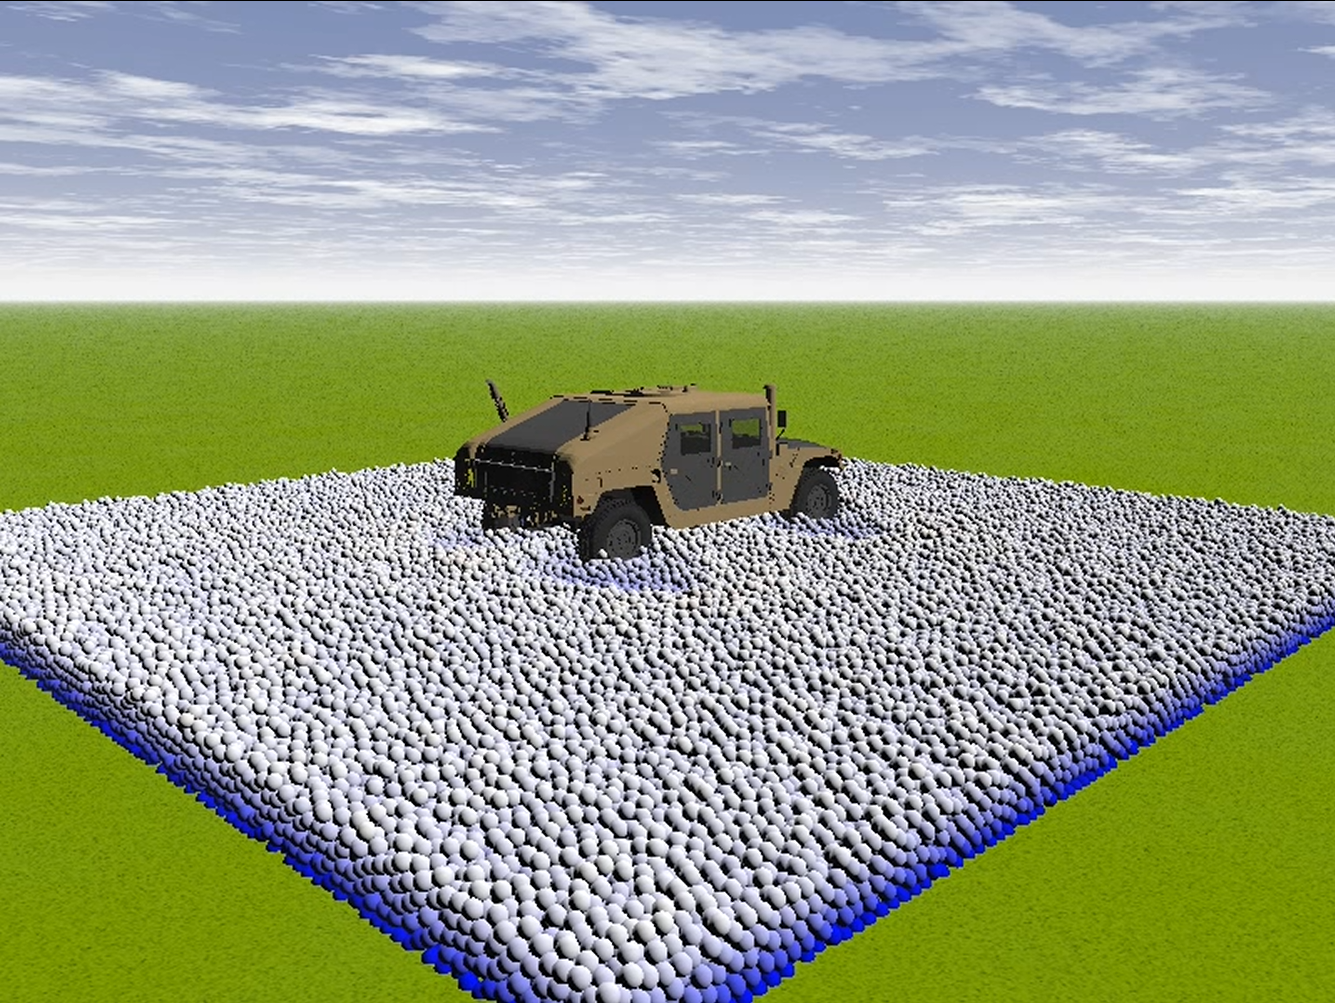
\includegraphics[width=\textwidth]{Figs/stuck.png}
		\caption{{\small HMMWV stuck in terrain of 6-DOF particles}}   
		\label{fig:stuck}
	\end{subfigure}
	\hfill
	\begin{subfigure}[b]{0.49\columnwidth}
		\centering
		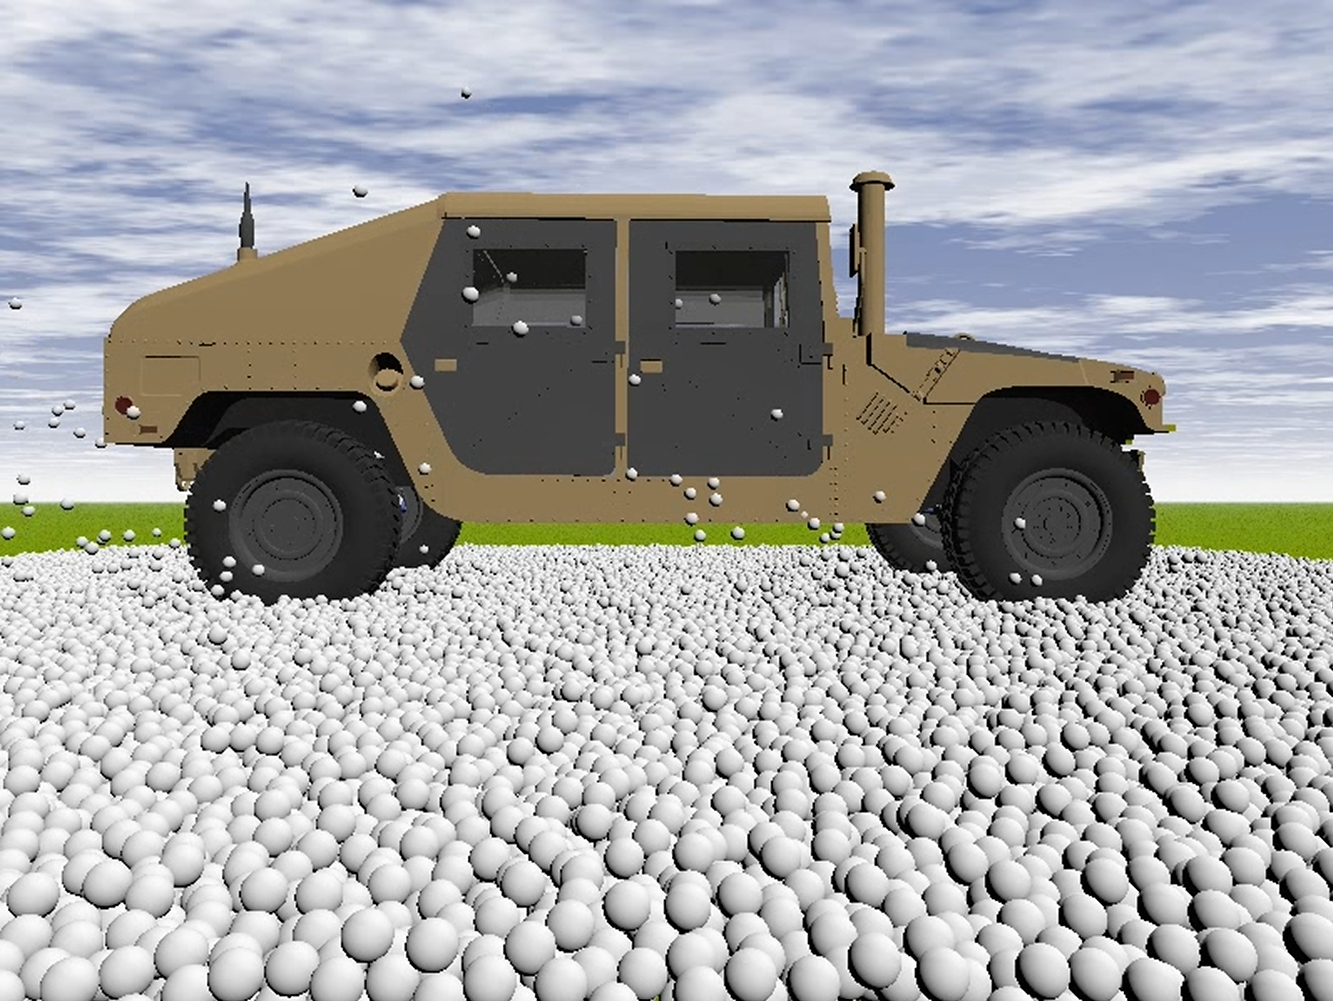
\includegraphics[width=\columnwidth]{Figs/HMMWV_spray.png}
		\caption{\small HMMWV remains in initial location spinning wheels and spraying particles backwards}   
		\label{fig:spray}
	\end{subfigure}
	\caption{\small HMMWV unable to make forward progress in 6-DOF particle field}
	\label{fig:spinOut}
\end{figure}

Future research can explore the cases where the vehicle remained stuck in its initial location. This occurred when the terrain was modeled as full 6-DOF spheres instead of rotation restricted 3-DOF spheres. When simulations were performed to test vehicle performance on these rotating spheres with a macro-scale friction angle of $35^\circ-40^\circ$ which is typical of a wide range of dry natural and crushed sands, the vehicle initialized and dropped onto the terrain normally, but throttle commands simply resulted in the vehicle spinning its tires in place. The vehicle would make no forward progress and instead continue to spin its tires while launching particles backwards. This case is visualized in Figure \ref{fig:spinOut}. This behavior provides an interesting research topic. The issue of the vehicle being unable to move from this point can be attributed to four possible different reason. First, this method of modeling dry sand with 6-DOF particles is incorrect and therefore we are not accurately simulating dry sand. This is possible since particles are not actually smooth spheres but instead have coarser jagged geometries which would result in more rolling friction. Second, the vehicle tires are not modeled correctly and something other than rigid tires should be used. Third, the controller does not account for how much tractive capabilities the terrain provides and is simply failing to pull the vehicle out of the sand trap. Finally fourth, all of the modeling in this scenario is correct and this behavior is what one would actually experience if they attempted to drive a HMMWV on loose dry sand aggressively. Research devoted to modeling and simulating dry loose sands as well as developing a controller to navigate the vehicle out and along that terrain would be an important development in the terramechanics and controls community. 

The research performed here would benefit greatly from physical tests to compliment the results of this study. Insight would be gained relating to hardware and computational speeds necessary to implement this controller on a physical vehicle. Overall the terramechanics field is a highly active and current area of research. The research performed in this study promotes the opportunity for many equally exciting research opportunities building off the results of this thesis.


%% ============================================================
\newpage
\titlespacing{\chapter}{0in}{-20pt}{0.2in}
\addcontentsline{toc}{chapter}{BIBLIOGRAPHY}

\begin{singlespacing}
\bibliographystyle{unsrt}
\bibliography{references}
\end{singlespacing}

%% ============================================================

\end{document}



